
\clearpage
\section{Collections}
\label{sec:tasks-feature-collections}

A collection brings work together. Open a shared collection for team work or a personal collection for your own organization.

\textbf{Where and who:} Tasks → Collections. For the person organizing work.

\begin{rcnote}[Example: Horizon]
Sarah uses a “Horizon visits” collection for visit preparation. Omar finds the work there instead of searching through several conversations.
\end{rcnote}

\begin{figure}[H]
\centering
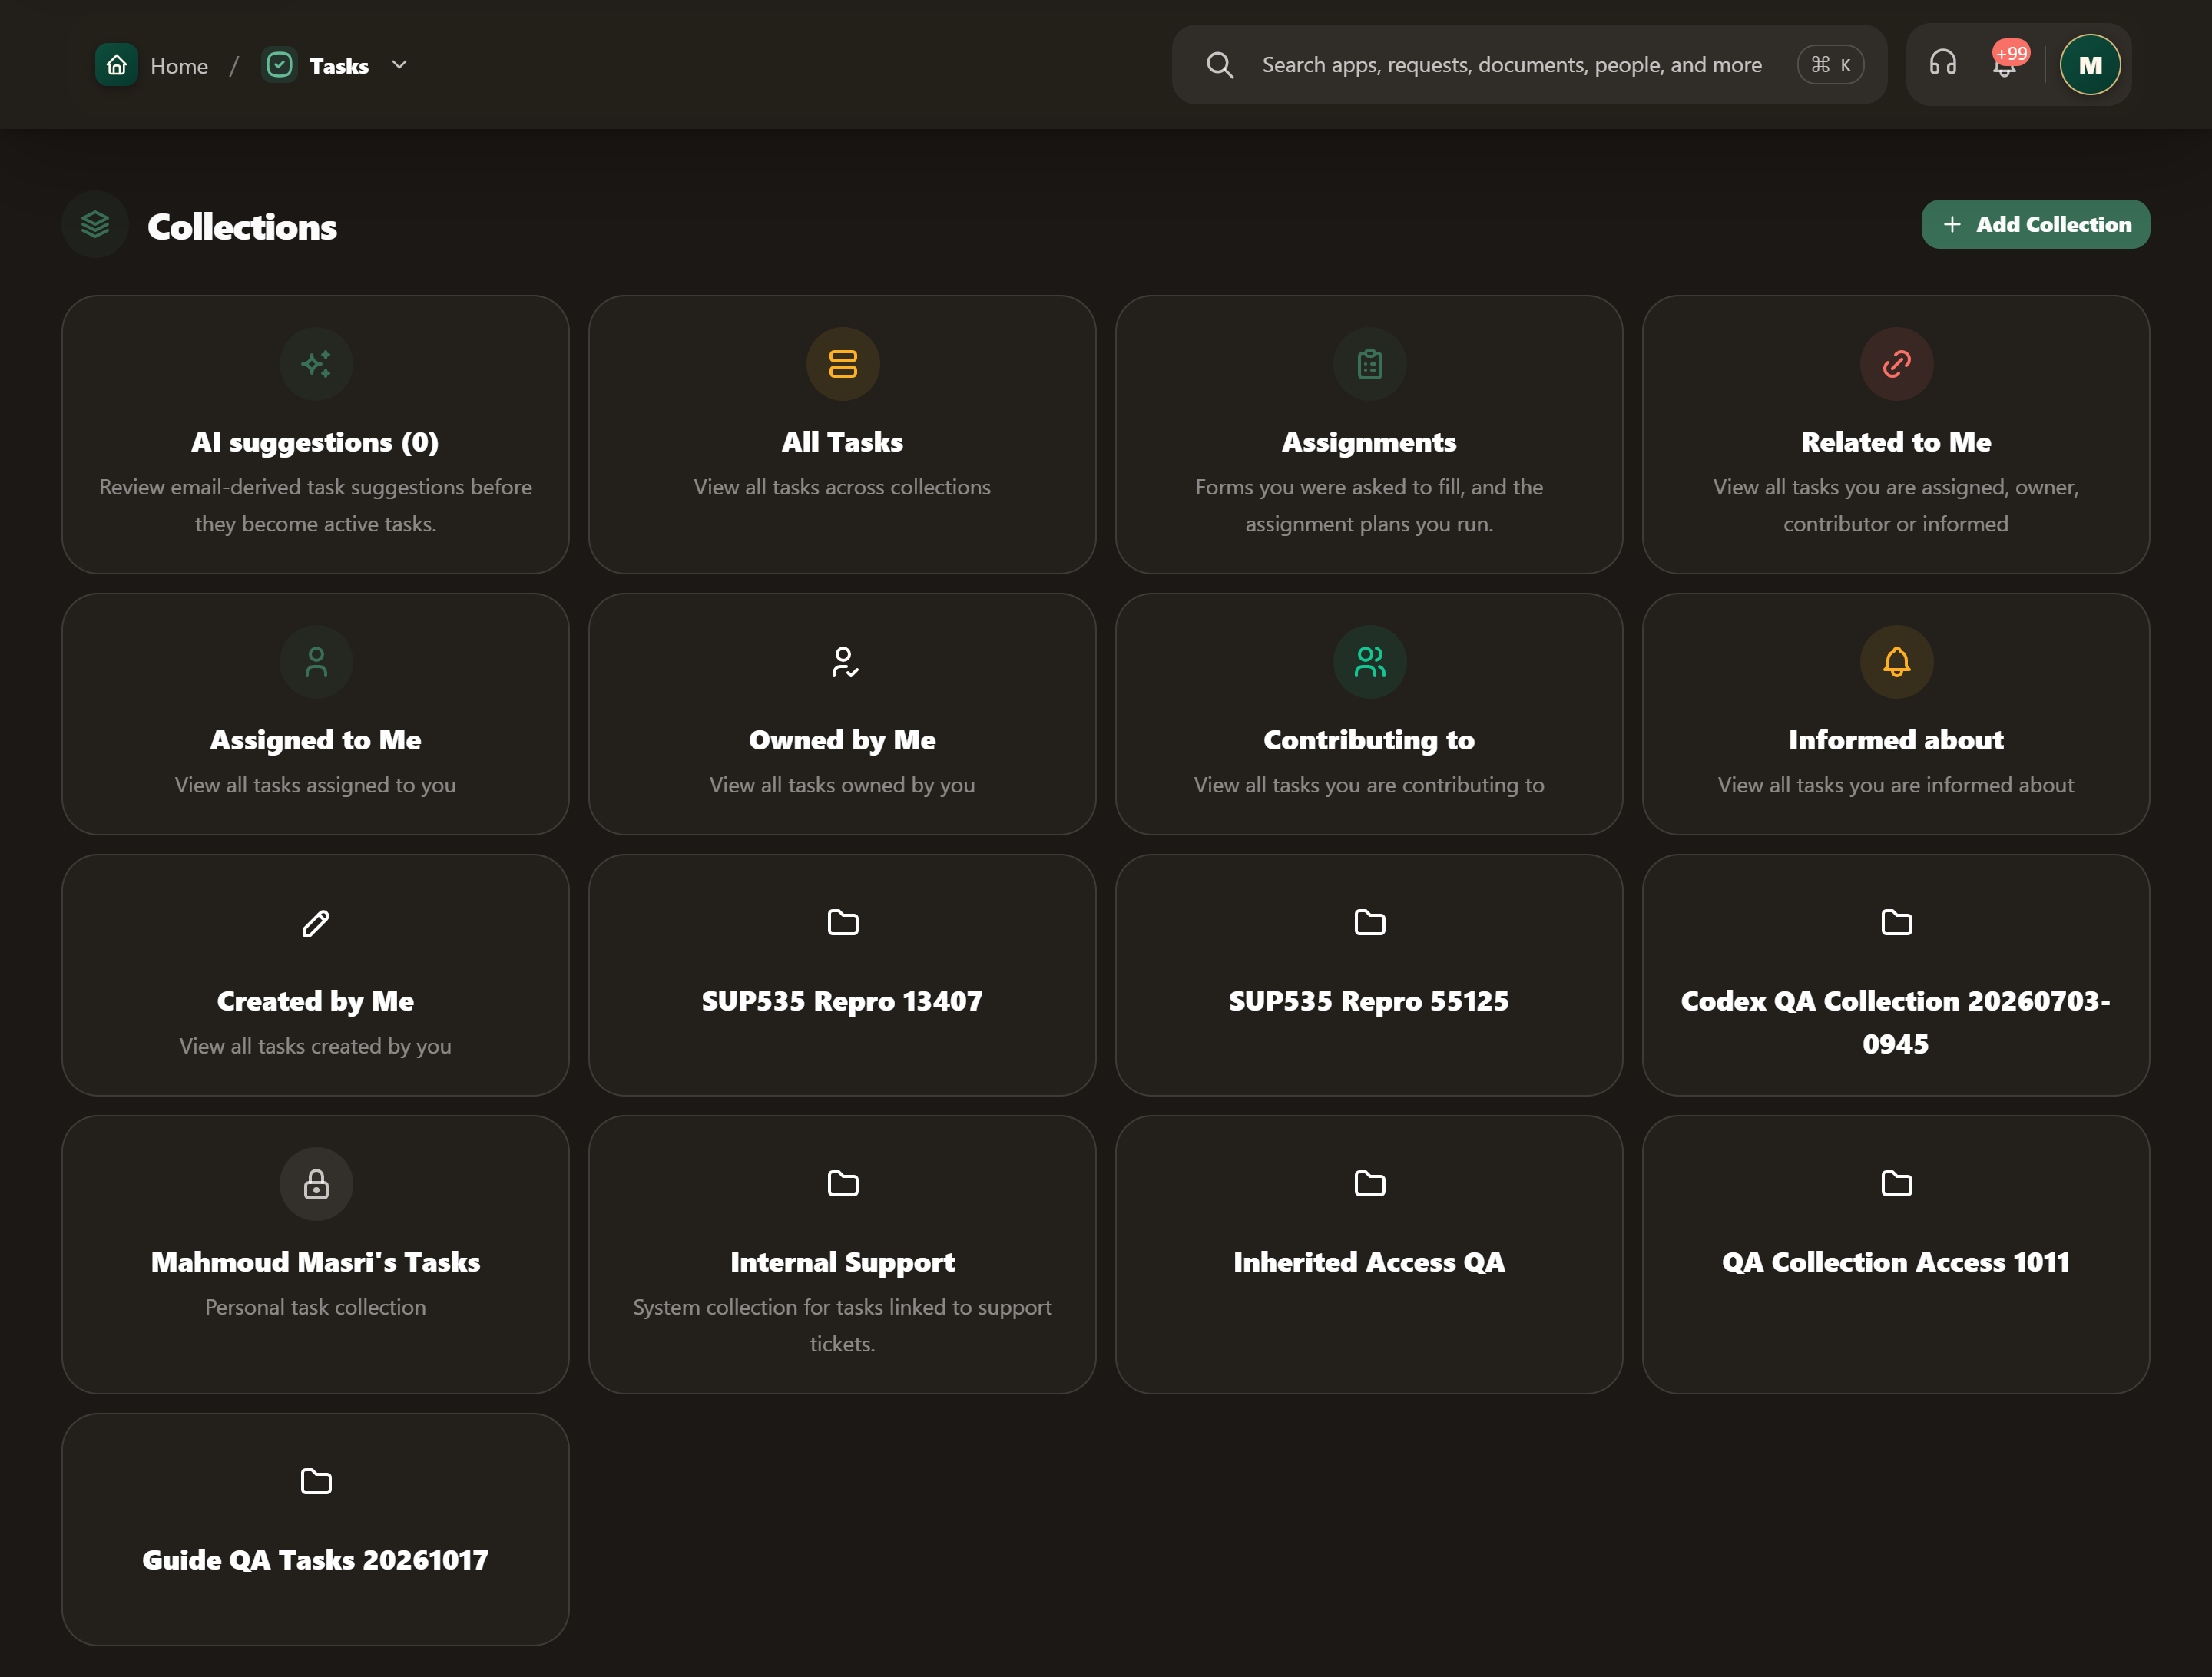
\includegraphics[width=0.95\linewidth,height=0.72\textheight,keepaspectratio]{figures/screens/ch04-collections-en.png}
\caption{Collections and available views}
\label{fig:tasks-collections-collections}
\shotnote{The Collections page offers two ways into work: personal view cards such as Assigned to Me, Assignments and AI suggestions, followed by the collections you can access. Start from a view when looking for your own work, and from a collection when following a particular team. The collections shown are test2 collections.}
\end{figure}

\begin{figure}[H]
\centering
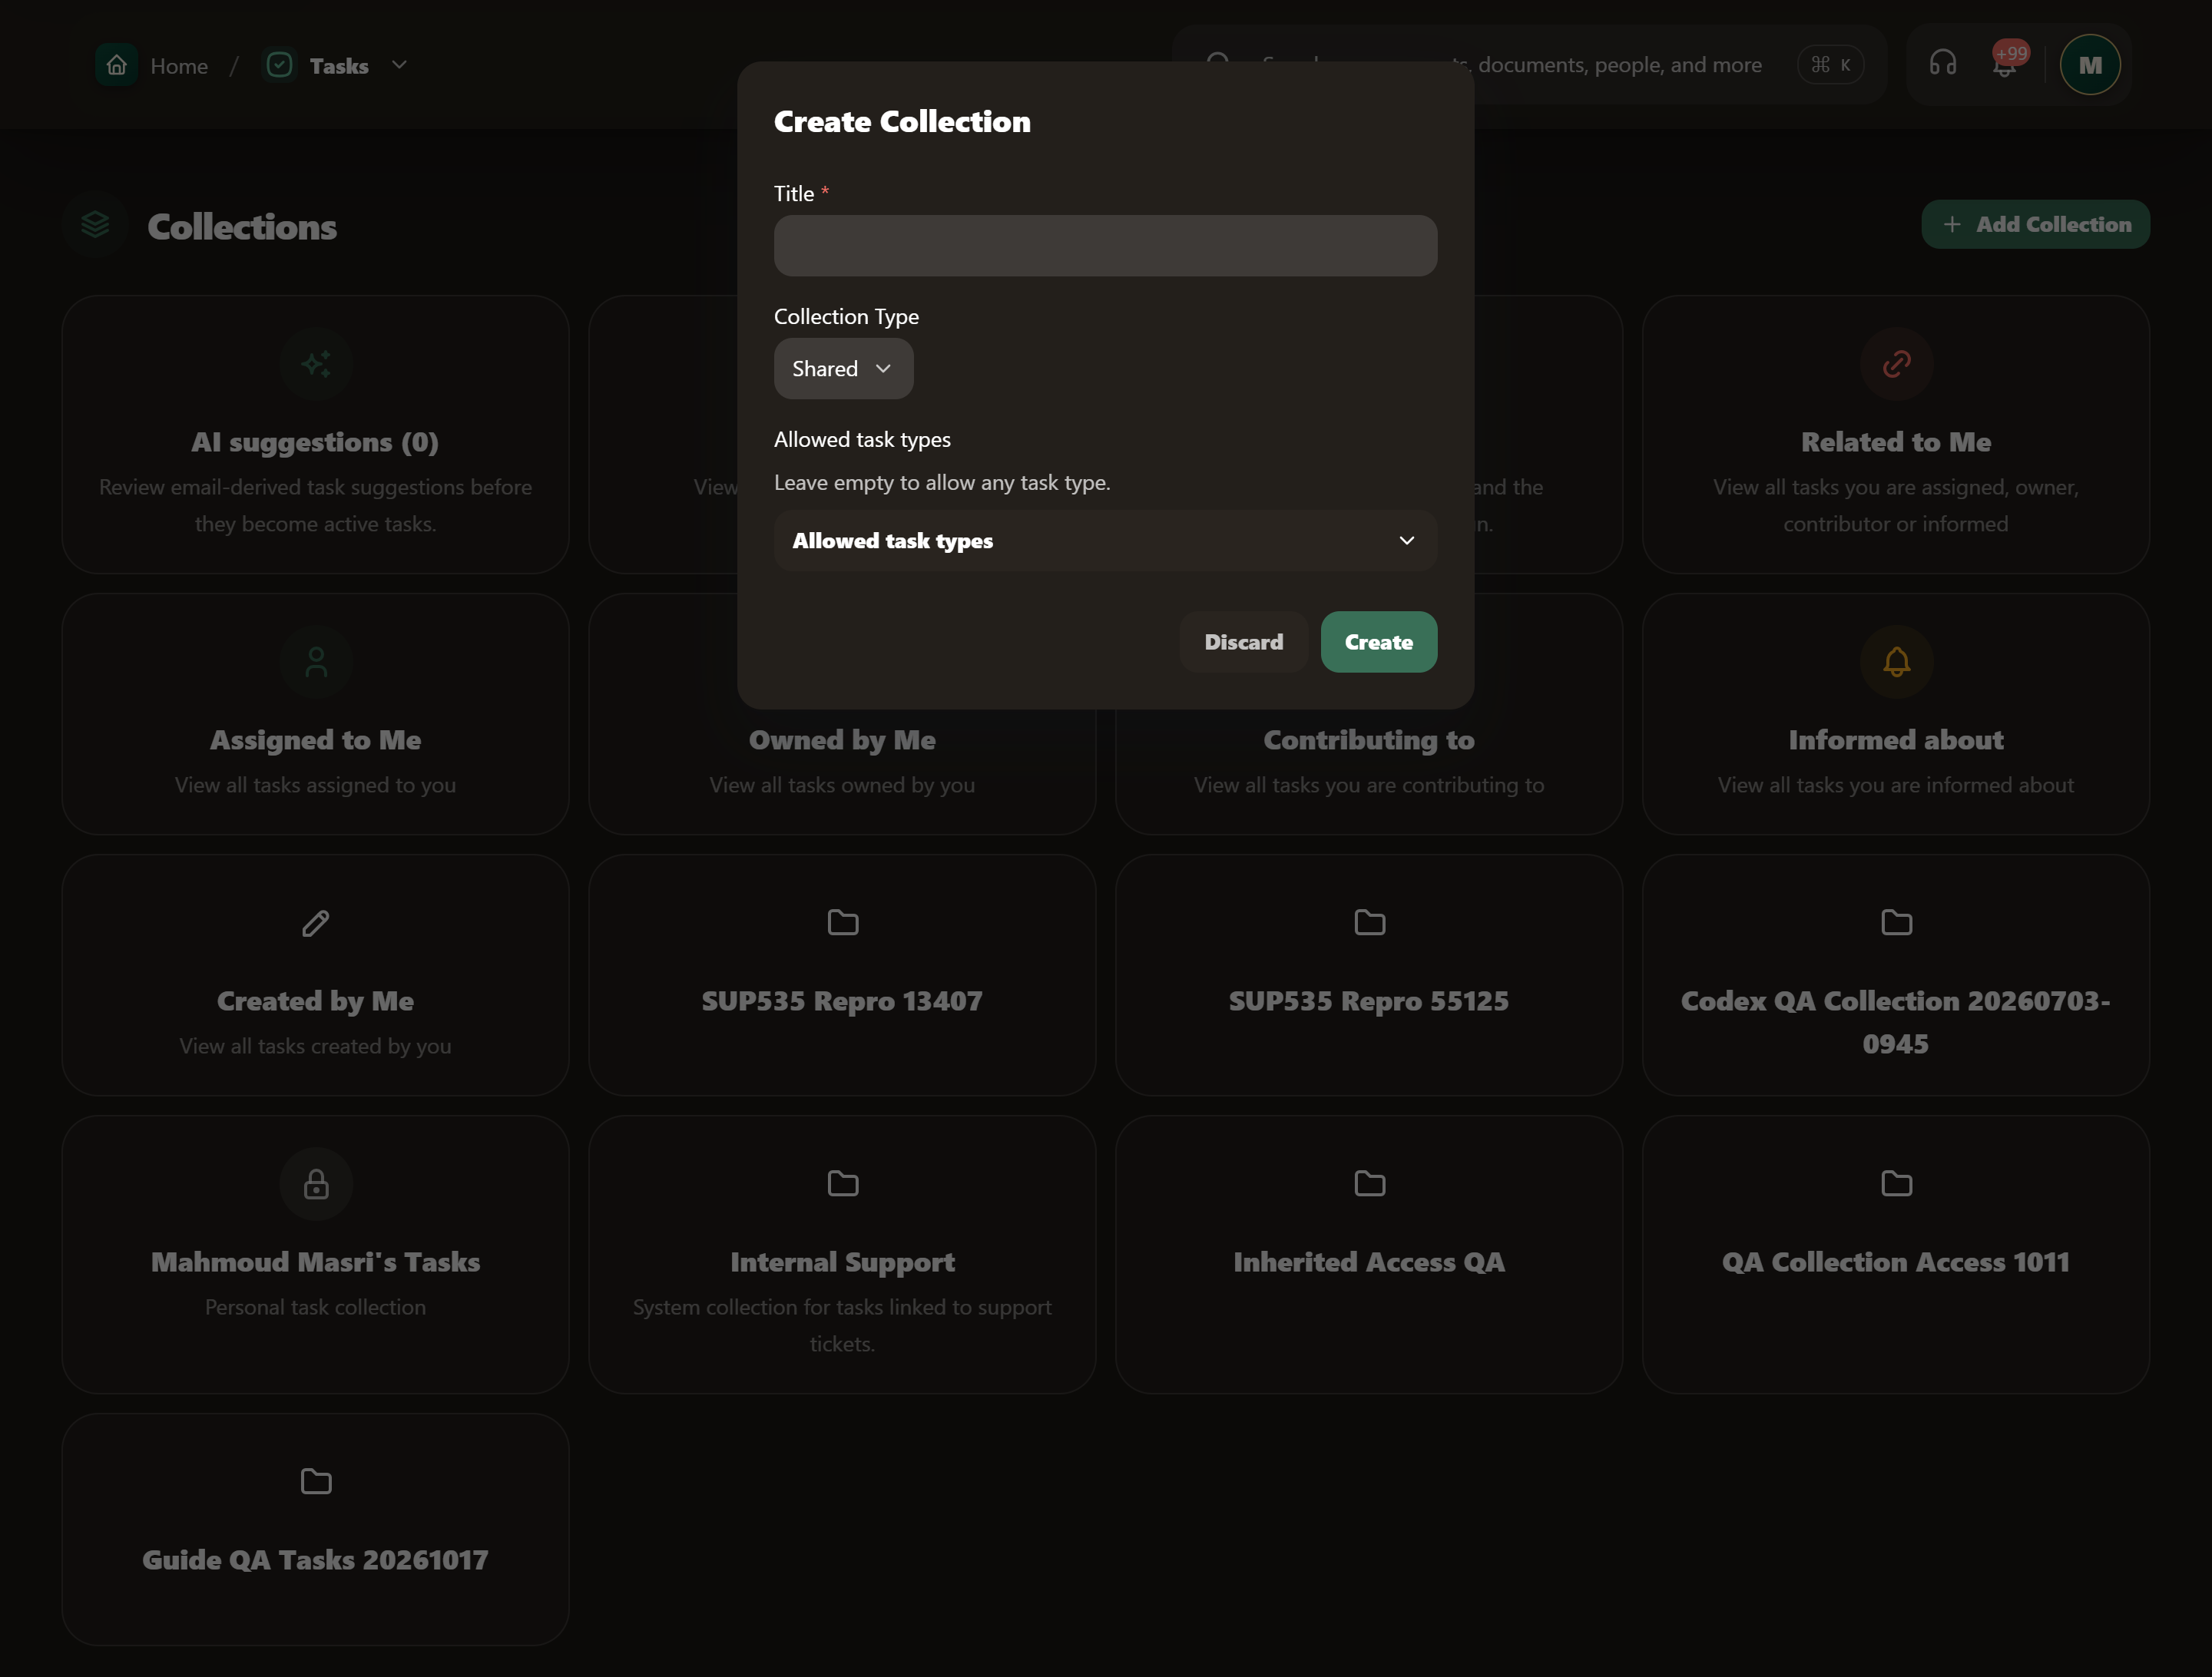
\includegraphics[width=0.95\linewidth,height=0.72\textheight,keepaspectratio]{figures/screens/ch04-collection-form-en.png}
\caption{Create collection form before saving}
\label{fig:tasks-collections-collection-form}
\shotnote{A collection needs only the required Title and a Collection type, which makes it shared or personal. Allowed task types is an optional restriction: leave it empty to accept any type available to you, or select types to limit the collection to them.}
\end{figure}

\begin{table}[H]
\centering
\caption{What can you record or do?}
\label{tab:tasks-collections-data}
\begin{tabularx}{\linewidth}{R{3.6cm} Y}
\rcHeaderRow
\thh{Section} & \thh{Content and action}\\
Title and type & A title is required. Type distinguishes personal and shared collections.\\
Allowed task types & An optional restriction on types in the collection; it does not grant permission to create a restricted type.\\
Collection settings & Edit details and types and manage sharing as permitted. Check team access before relying on it.\\
\end{tabularx}
\end{table}

\begin{figure}[H]
\centering
\begin{tikzpicture}[node distance=0.5cm]
\node[stepBox] (a) {\RL{Choose collection}};
\node[stepBox,below=of a] (b) {\RL{Check access}};
\node[stepBox,below=of b] (c) {\RL{Open team tasks}};
\draw[flowsTo] (a) -- (b);
\draw[flowsTo] (b) -- (c);
\end{tikzpicture}
\rclegend
\caption{Steps to follow}
\label{fig:tasks-collections-flow}
\shotnote{The diagram places the access check between choosing a collection and distributing tasks, because your own access does not guarantee the team can see it. Work distributed in a collection the assignees cannot reach will not be found by them.}
\end{figure}

\subsection{Steps and verification}
\begin{enumerate}
\item Look for the intended collection first. To create one, choose “Add Collection”.
\item Enter a clear title, choose the collection type and allowed types if needed, then “Create”.
\item Open the collection card. Before assigning work, verify that the intended team members can open it.
\end{enumerate}

\textbf{Check and recovery:} The collection title should appear when opened. If “Collection not available” appears, return to Collections, refresh and have sharing and access checked; do not create duplicates.

\clearpage
\section{Task views}
\label{sec:tasks-feature-views}

A view changes how you find and review tasks. Use the list for details, the board for status, and Check-ins for team updates.

\textbf{Where and who:} Tasks → a collection or a personal view. For daily employee and manager review.

\begin{rcnote}[Example: Horizon]
Omar opens Assigned to Me to find his work. Sarah reviews the Horizon visits board to see what has not started.
\end{rcnote}

\begin{figure}[H]
\centering
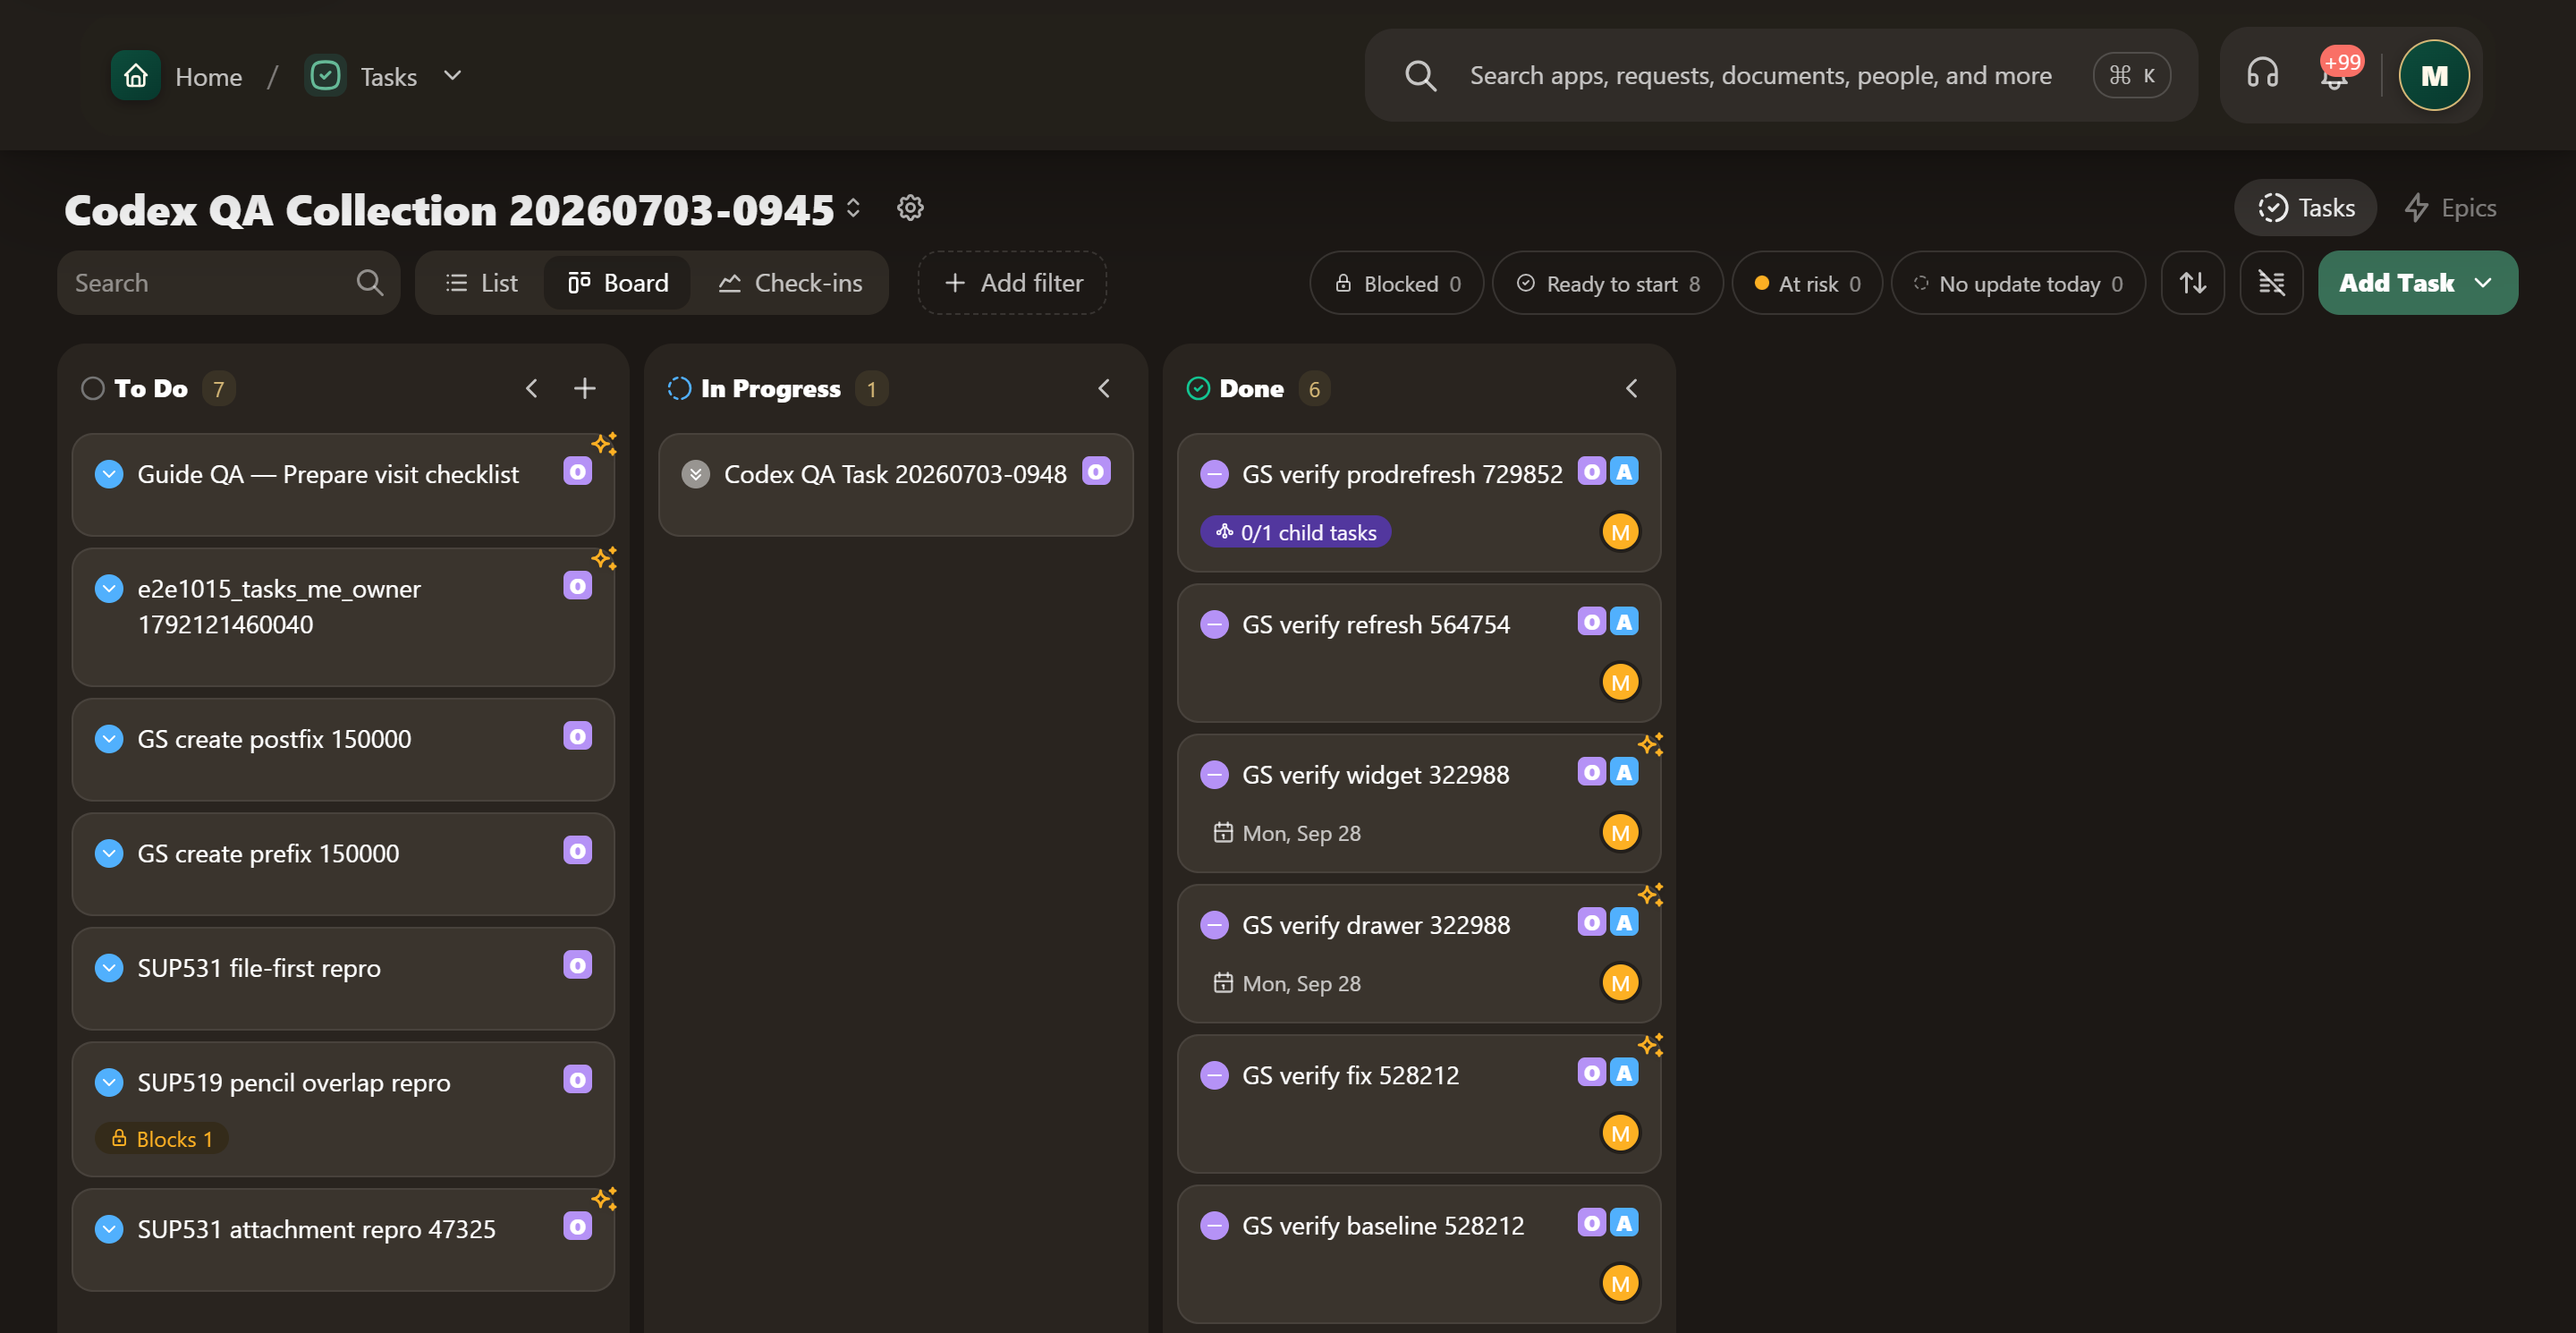
\includegraphics[width=0.95\linewidth,height=0.72\textheight,keepaspectratio]{figures/screens/ch04-board-en.png}
\caption{A test collection board}
\label{fig:tasks-views-board}
\shotnote{The board shows the collection’s tasks in columns that represent statuses, such as To Do, In Progress and Done, so you can see at a glance where work stands and where it accumulates. Badges such as Blocked and Ready to start show how many tasks need attention. Seeing a task does not mean you can edit or move it.}
\end{figure}

\begin{figure}[H]
\centering
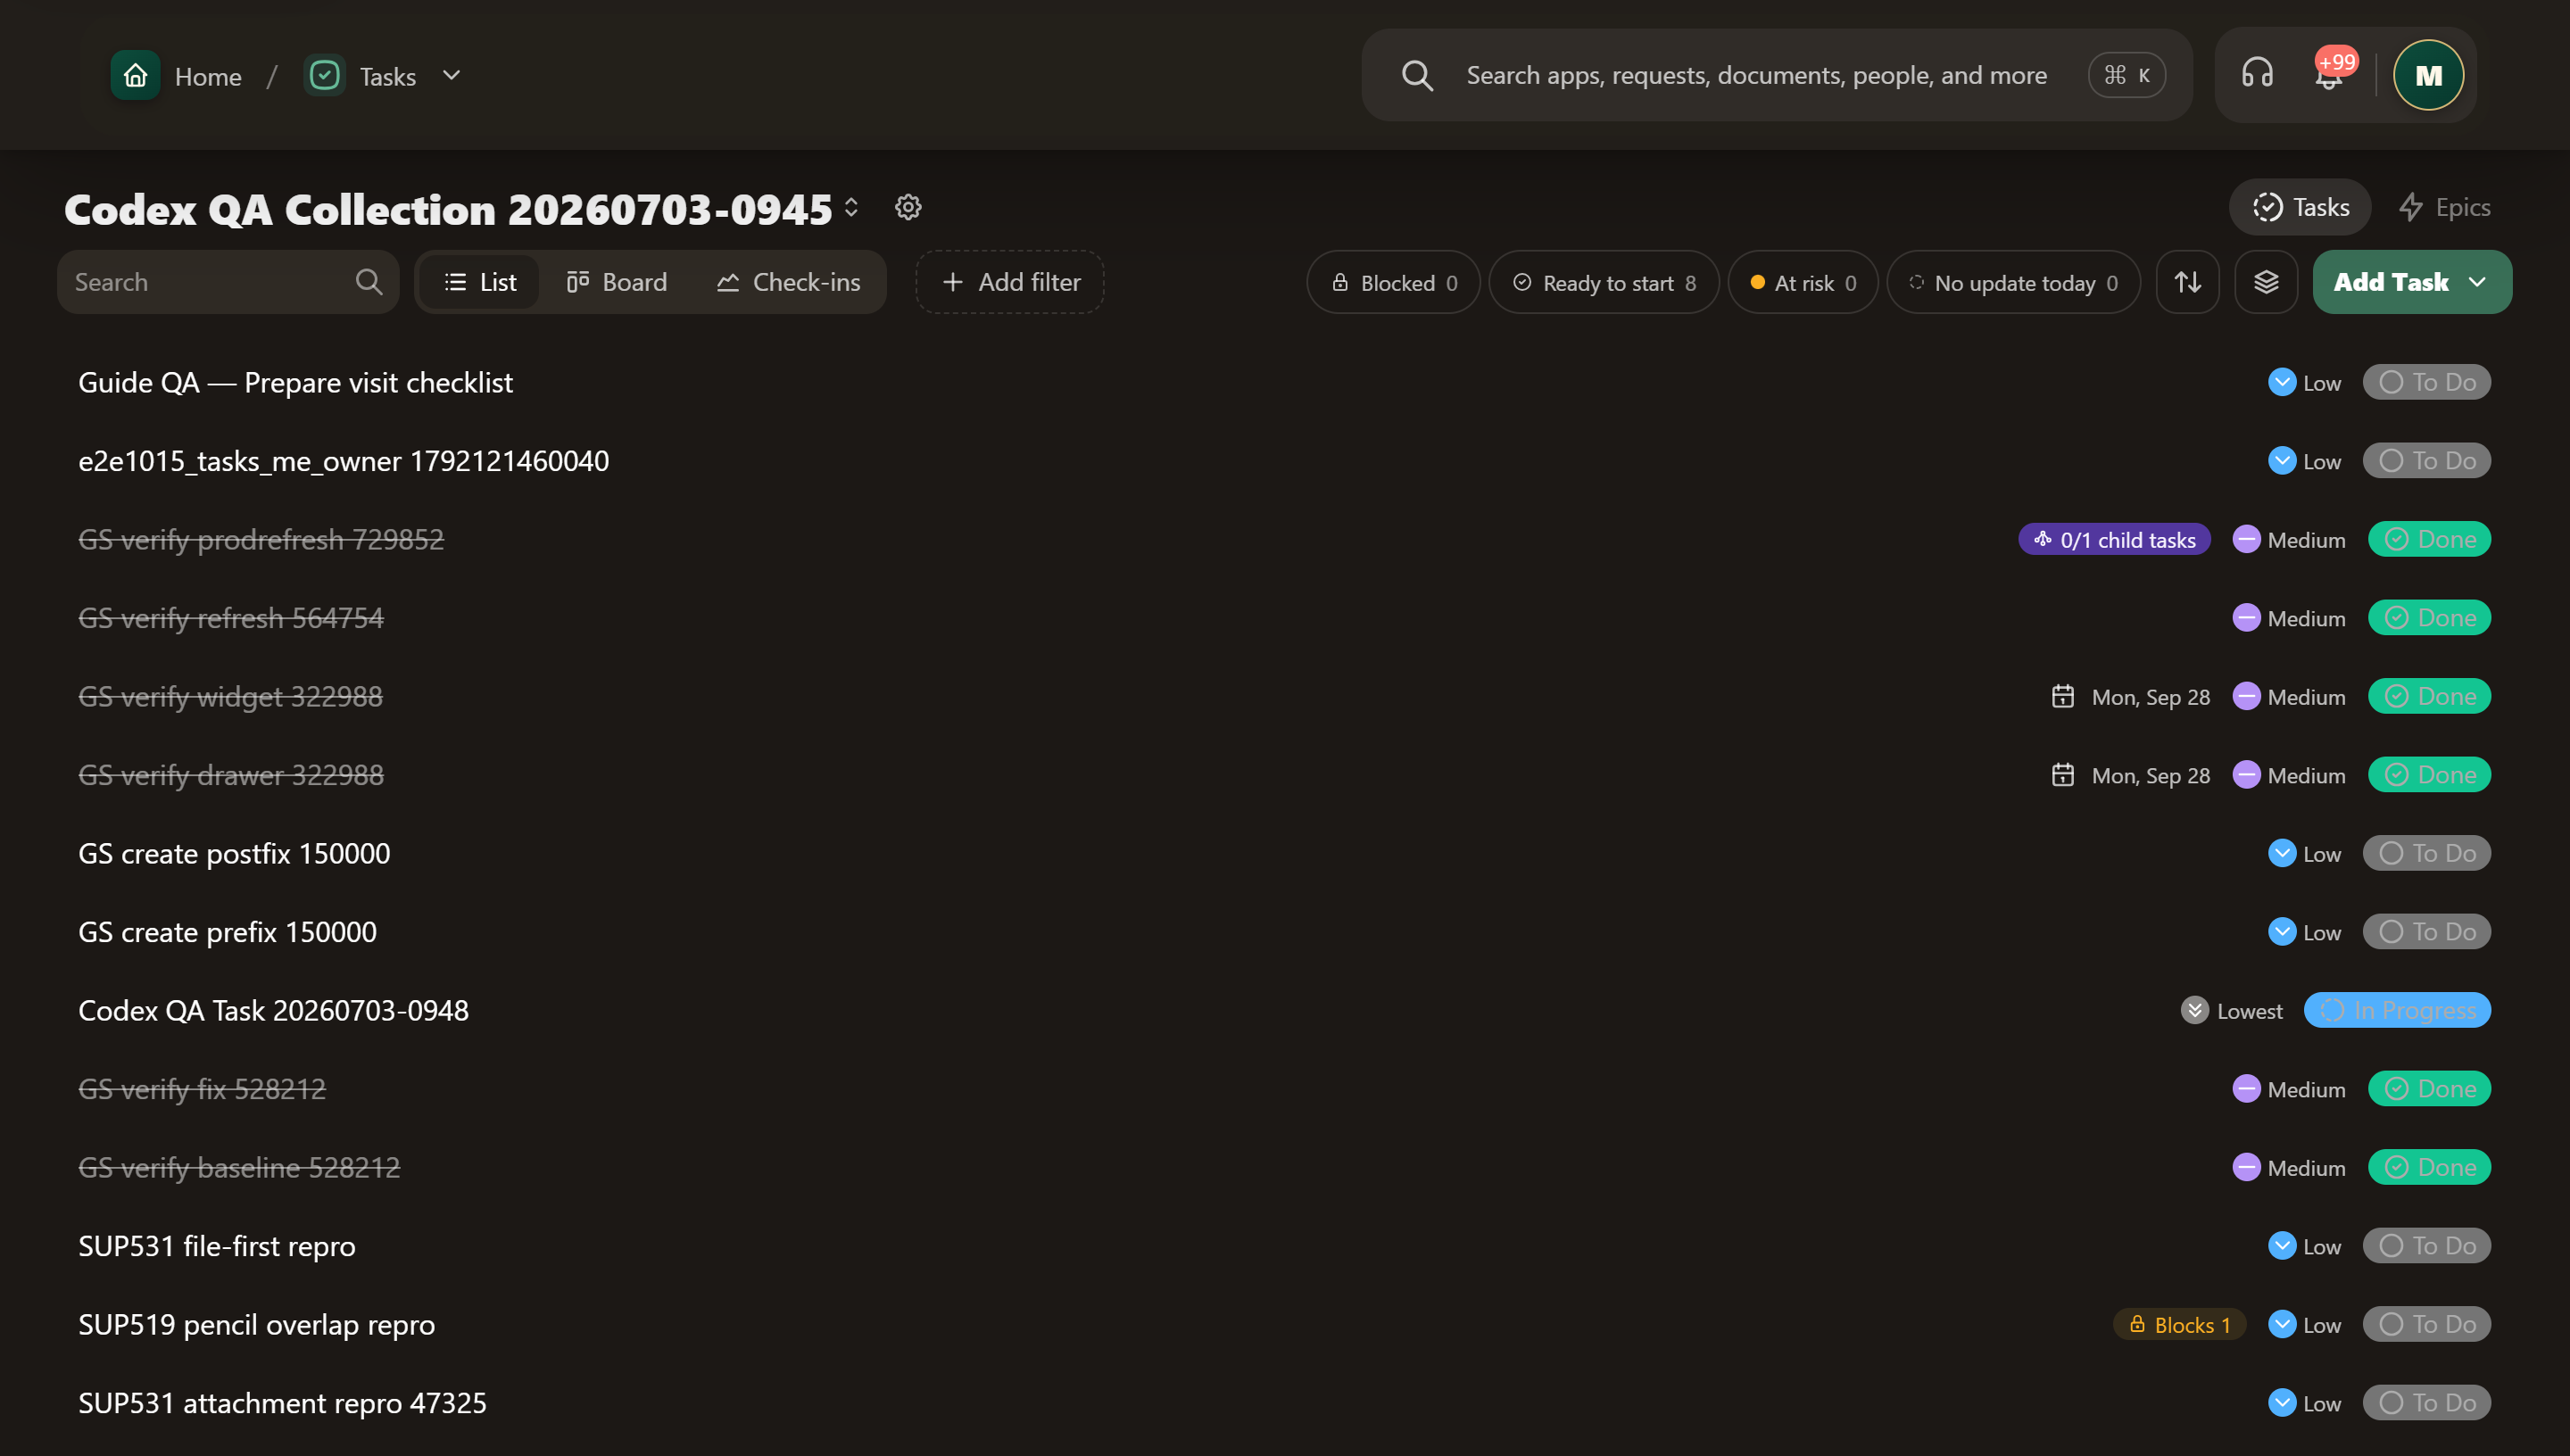
\includegraphics[width=0.95\linewidth,height=0.72\textheight,keepaspectratio]{figures/screens/ch04-list-en.png}
\caption{List view}
\label{fig:tasks-views-list}
\shotnote{The List view shows the same tasks as rows with each task’s status, priority and due date; completed tasks appear struck through. It suits comparing tasks and reviewing details, while search, Add filter and sorting narrow the results when there are many tasks.}
\end{figure}

\begin{figure}[H]
\centering
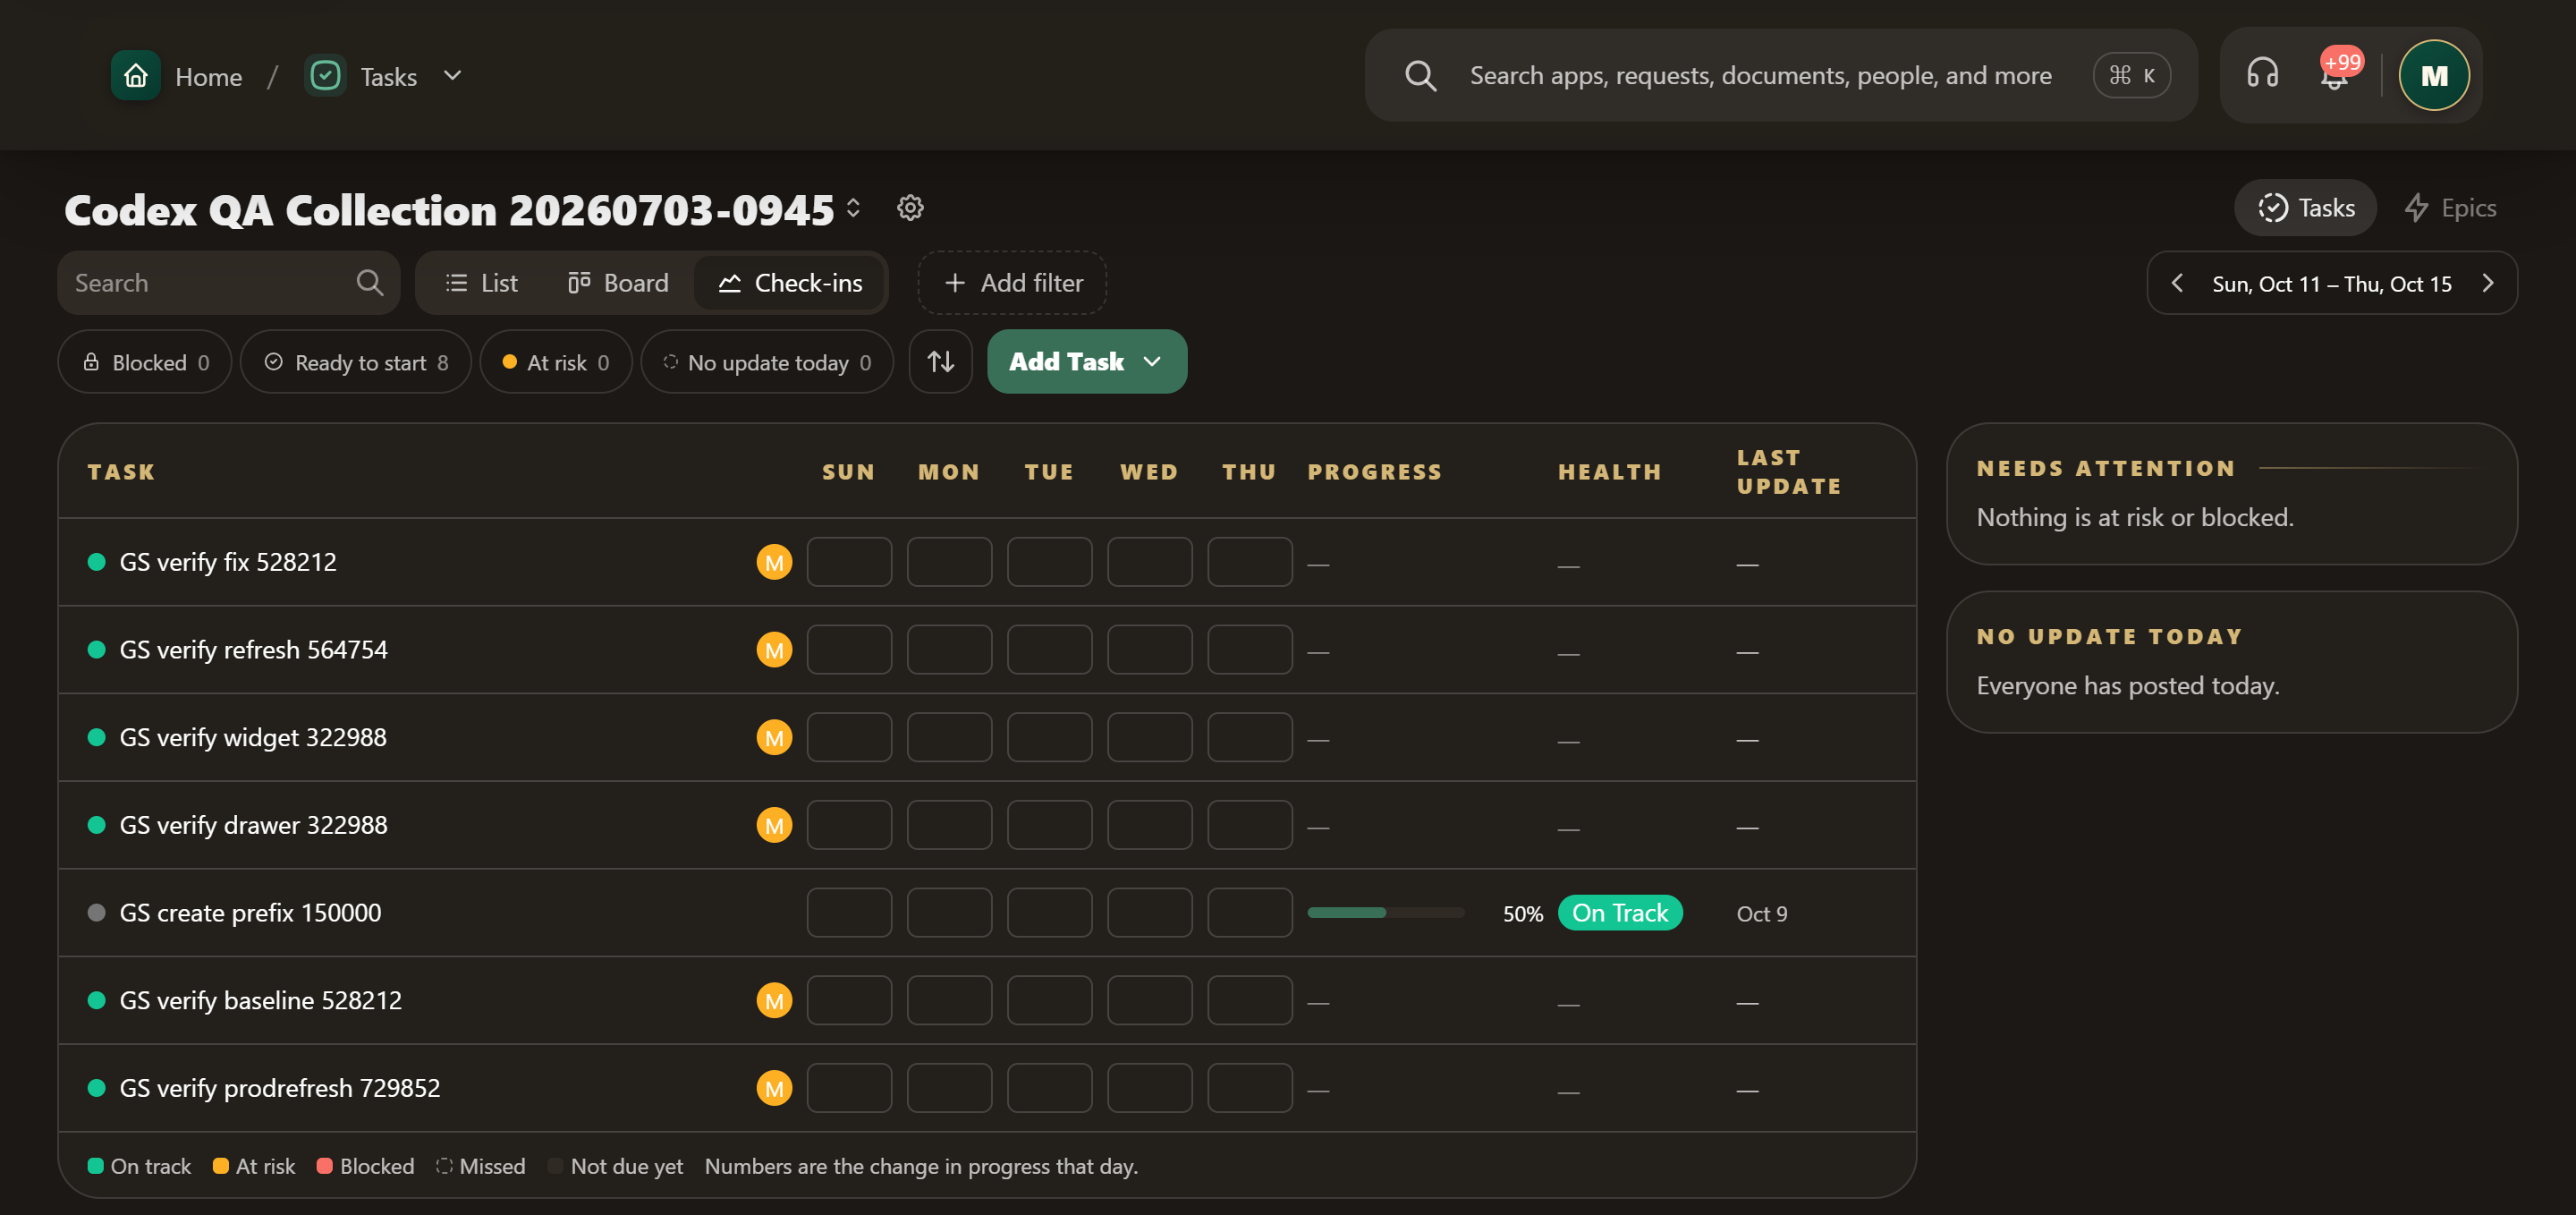
\includegraphics[width=0.95\linewidth,height=0.72\textheight,keepaspectratio]{figures/screens/ch04-checkins-en.png}
\caption{Check-ins view}
\label{fig:tasks-views-checkins}
\shotnote{Check-ins shows each task’s updates across the selected week, with progress, Health and last update. The Needs attention and No update today cards collect what requires follow-up. A missing update does not mean the task is complete, only that nobody has posted one.}
\end{figure}

\begin{table}[H]
\centering
\caption{What can you record or do?}
\label{tab:tasks-views-data}
\begin{tabularx}{\linewidth}{R{3.6cm} Y}
\rcHeaderRow
\thh{Section} & \thh{Content and action}\\
All Tasks; Related to Me & The first collects accessible work; the second focuses on your involvement.\\
Assigned to Me; Owned by Me & Work assigned to you versus work whose outcome you own.\\
Contributing to; Informed about; Created by Me & Separate views for contribution, awareness and authorship.\\
Search, filters and views & Search by title; filter, sort and group using available options. Bulk board actions depend on task permissions and valid transitions.\\
\end{tabularx}
\end{table}

\begin{figure}[H]
\centering
\begin{tikzpicture}[node distance=0.5cm]
\node[stepBox] (a) {\RL{Choose role}\\\RL{or collection}};
\node[stepBox,below=of a] (b) {\RL{Search and filter}};
\node[stepBox,below=of b] (c) {\RL{Open task}};
\draw[flowsTo] (a) -- (b);
\draw[flowsTo] (b) -- (c);
\end{tikzpicture}
\rclegend
\caption{Steps to follow}
\label{fig:tasks-views-flow}
\shotnote{The diagram shows the search order: start with the view matching your role or the collection you follow, narrow the results, then open the task. Starting from a view that is not yours can make a task seem missing when it is in another view.}
\end{figure}

\subsection{Steps and verification}
\begin{enumerate}
\item Open the collection or view matching your role. Search for the task title.
\item Switch between List and Board; review filters before concluding a task is missing.
\item Open the task card; if an action menu appears, choose Open. Review status and responsibility.
\end{enumerate}

\textbf{Check and recovery:} If work is missing, clear filters and check collection, role and access. Switching views does not change work status.

\clearpage
\section{Create a task and review details}
\label{sec:tasks-feature-details}

A task records a required outcome and who handles it. Write a specific title, then set responsibility, timing and the information needed to act.

\textbf{Where and who:} Tasks → collection → Add Task. For people assigning and doing work.

\begin{rcnote}[Example: Horizon]
Sarah creates “Prepare visit checklist” in Horizon visits and assigns it to Omar before the visit. Sarah remains accountable for the outcome.
\end{rcnote}

\begin{figure}[H]
\centering
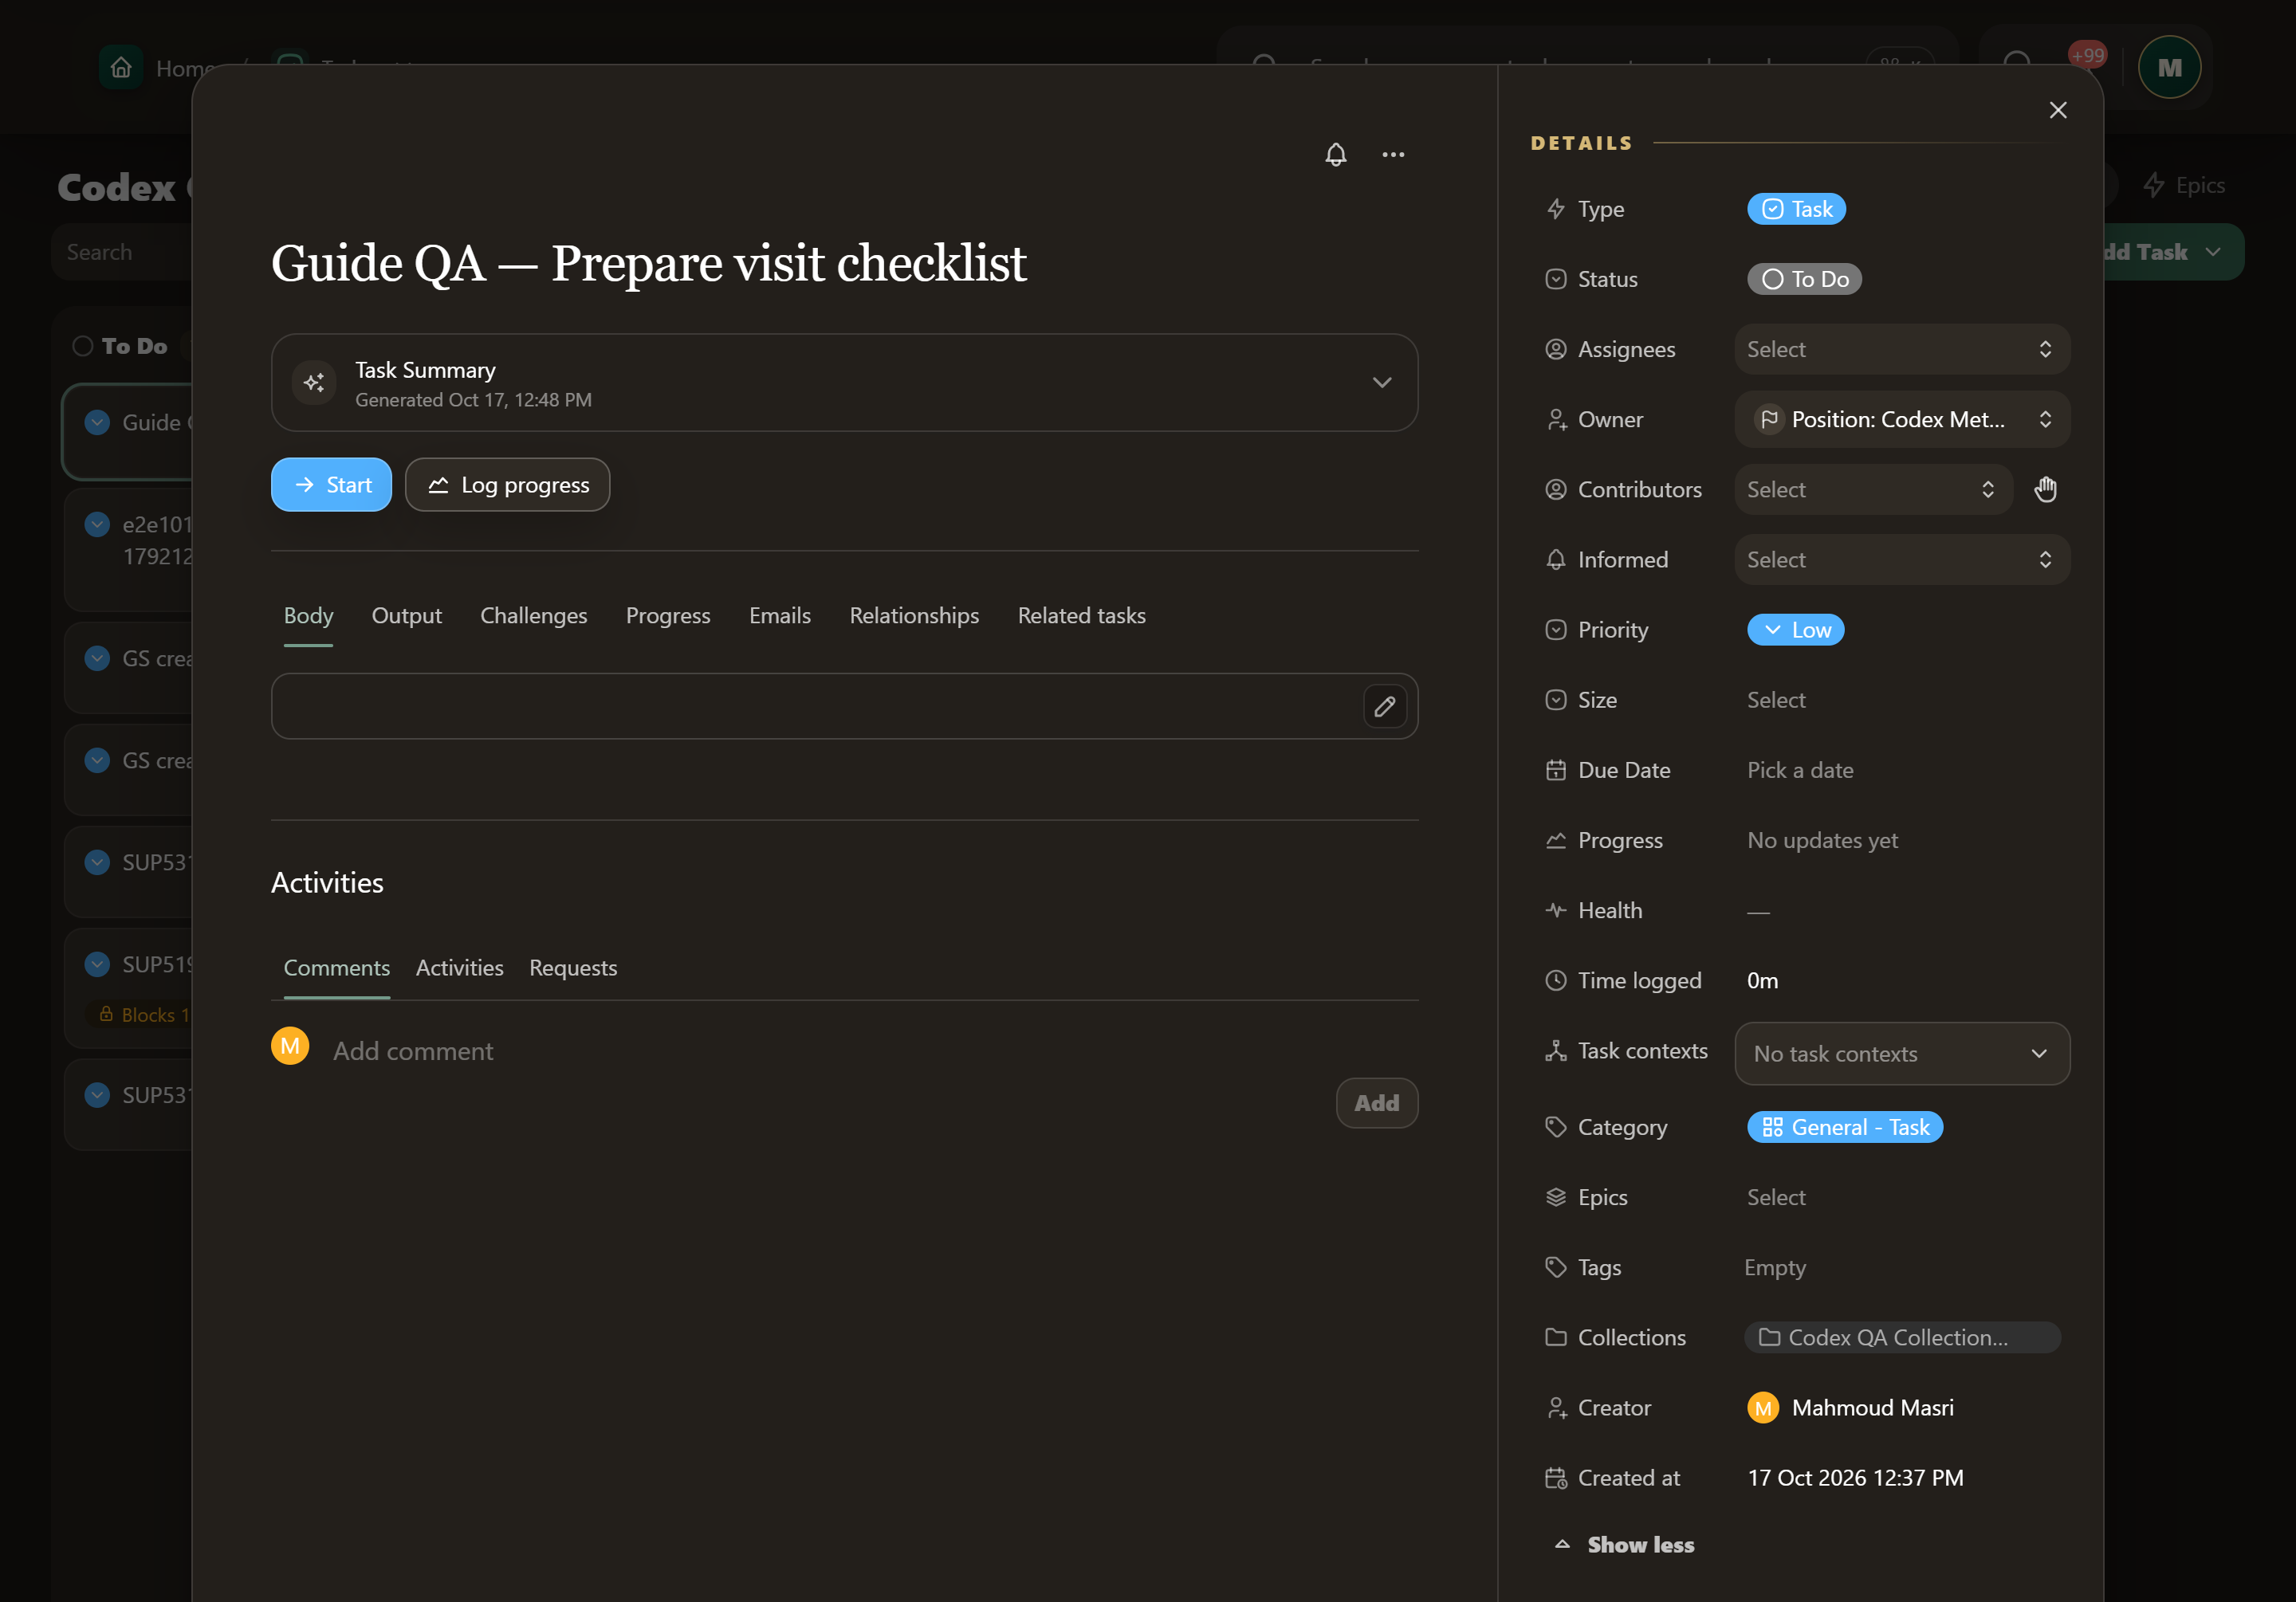
\includegraphics[width=0.95\linewidth,height=0.72\textheight,keepaspectratio]{figures/screens/ch04-details-en.png}
\caption{Details of a saved test task}
\label{fig:tasks-details-details}
\shotnote{The Details panel holds what defines responsibility and planning: who acts, who owns the outcome, who contributes or stays informed, then priority and due date. Show more reveals category, collections, creator and creation time; the system fills the last two. Note that the Owner can be a position rather than a person; this is a test2 task.}
\end{figure}

\begin{table}[H]
\centering
\caption{What can you record or do?}
\label{tab:tasks-details-data}
\begin{tabularx}{\linewidth}{R{3.6cm} Y}
\rcHeaderRow
\thh{Section} & \thh{Content and action}\\
Title, type and status & Title describes the outcome; type selects settings and rules; status reflects the work stage.\\
People & Assignees act; the owner is accountable; contributors supply work; informed people need awareness. Available selections may include members or positions.\\
Planning & Priority, size, due date and linked contexts. Choose what serves the task; not every link is required.\\
Show more & Category, epics, tags and collections. Creator and creation time are generated.\\
Content & Body, output and challenges; then progress, email and relationships where available. The next two pages explain these.\\
Sharing and deletion & More options offers sharing where permitted, or deletion with confirmation. Complete work to retain its history; deletion removes the task.\\
\end{tabularx}
\end{table}

\begin{figure}[H]
\centering
\begin{tikzpicture}[node distance=0.5cm]
\node[stepBox] (a) {\RL{Define outcome}};
\node[stepBox,below=of a] (b) {\RL{Set responsibility}\\\RL{and date}};
\node[stepBox,below=of b] (c) {\RL{Create and verify}};
\draw[flowsTo] (a) -- (b);
\draw[flowsTo] (b) -- (c);
\end{tikzpicture}
\rclegend
\caption{Steps to follow}
\label{fig:tasks-details-flow}
\shotnote{The diagram orders task creation in three steps: define the required outcome, set who handles it and when, then create and verify. A clear title makes choosing the right assignee easier, and reopening the task confirms its details were saved as intended.}
\end{figure}

\subsection{Steps and verification}
\begin{enumerate}
\item Choose Add Task, then an available type. Enter an outcome-focused title and body.
\item Set assignee and owner, and due date and priority as needed. Review required relationships before creation.
\item Choose Create. Reopen from the list or board and verify title, responsibility and status.
\item On a saved task, wait for save confirmation after editing fields. Use the text editor’s save action, then reopen to confirm persistence.
\end{enumerate}

\textbf{Check and recovery:} If saving is blocked, check the error, type, required relationships and permission. Closing the dialog alone does not prove the text was saved.

\clearpage
\section{Progress, results and discussion}
\label{sec:tasks-feature-follow-up}

A task collects results, obstacles and requests between colleagues. Keep its outcome and status current so another person can continue without guessing.

\textbf{Where and who:} Open a saved task; use content and activity tabs. For assignees, contributors and owners.

\begin{rcnote}[Example: Horizon]
Omar records the checklist preparation and notes that the site address is still missing. Sarah reviews the blocker and agrees the next step.
\end{rcnote}

\begin{figure}[H]
\centering
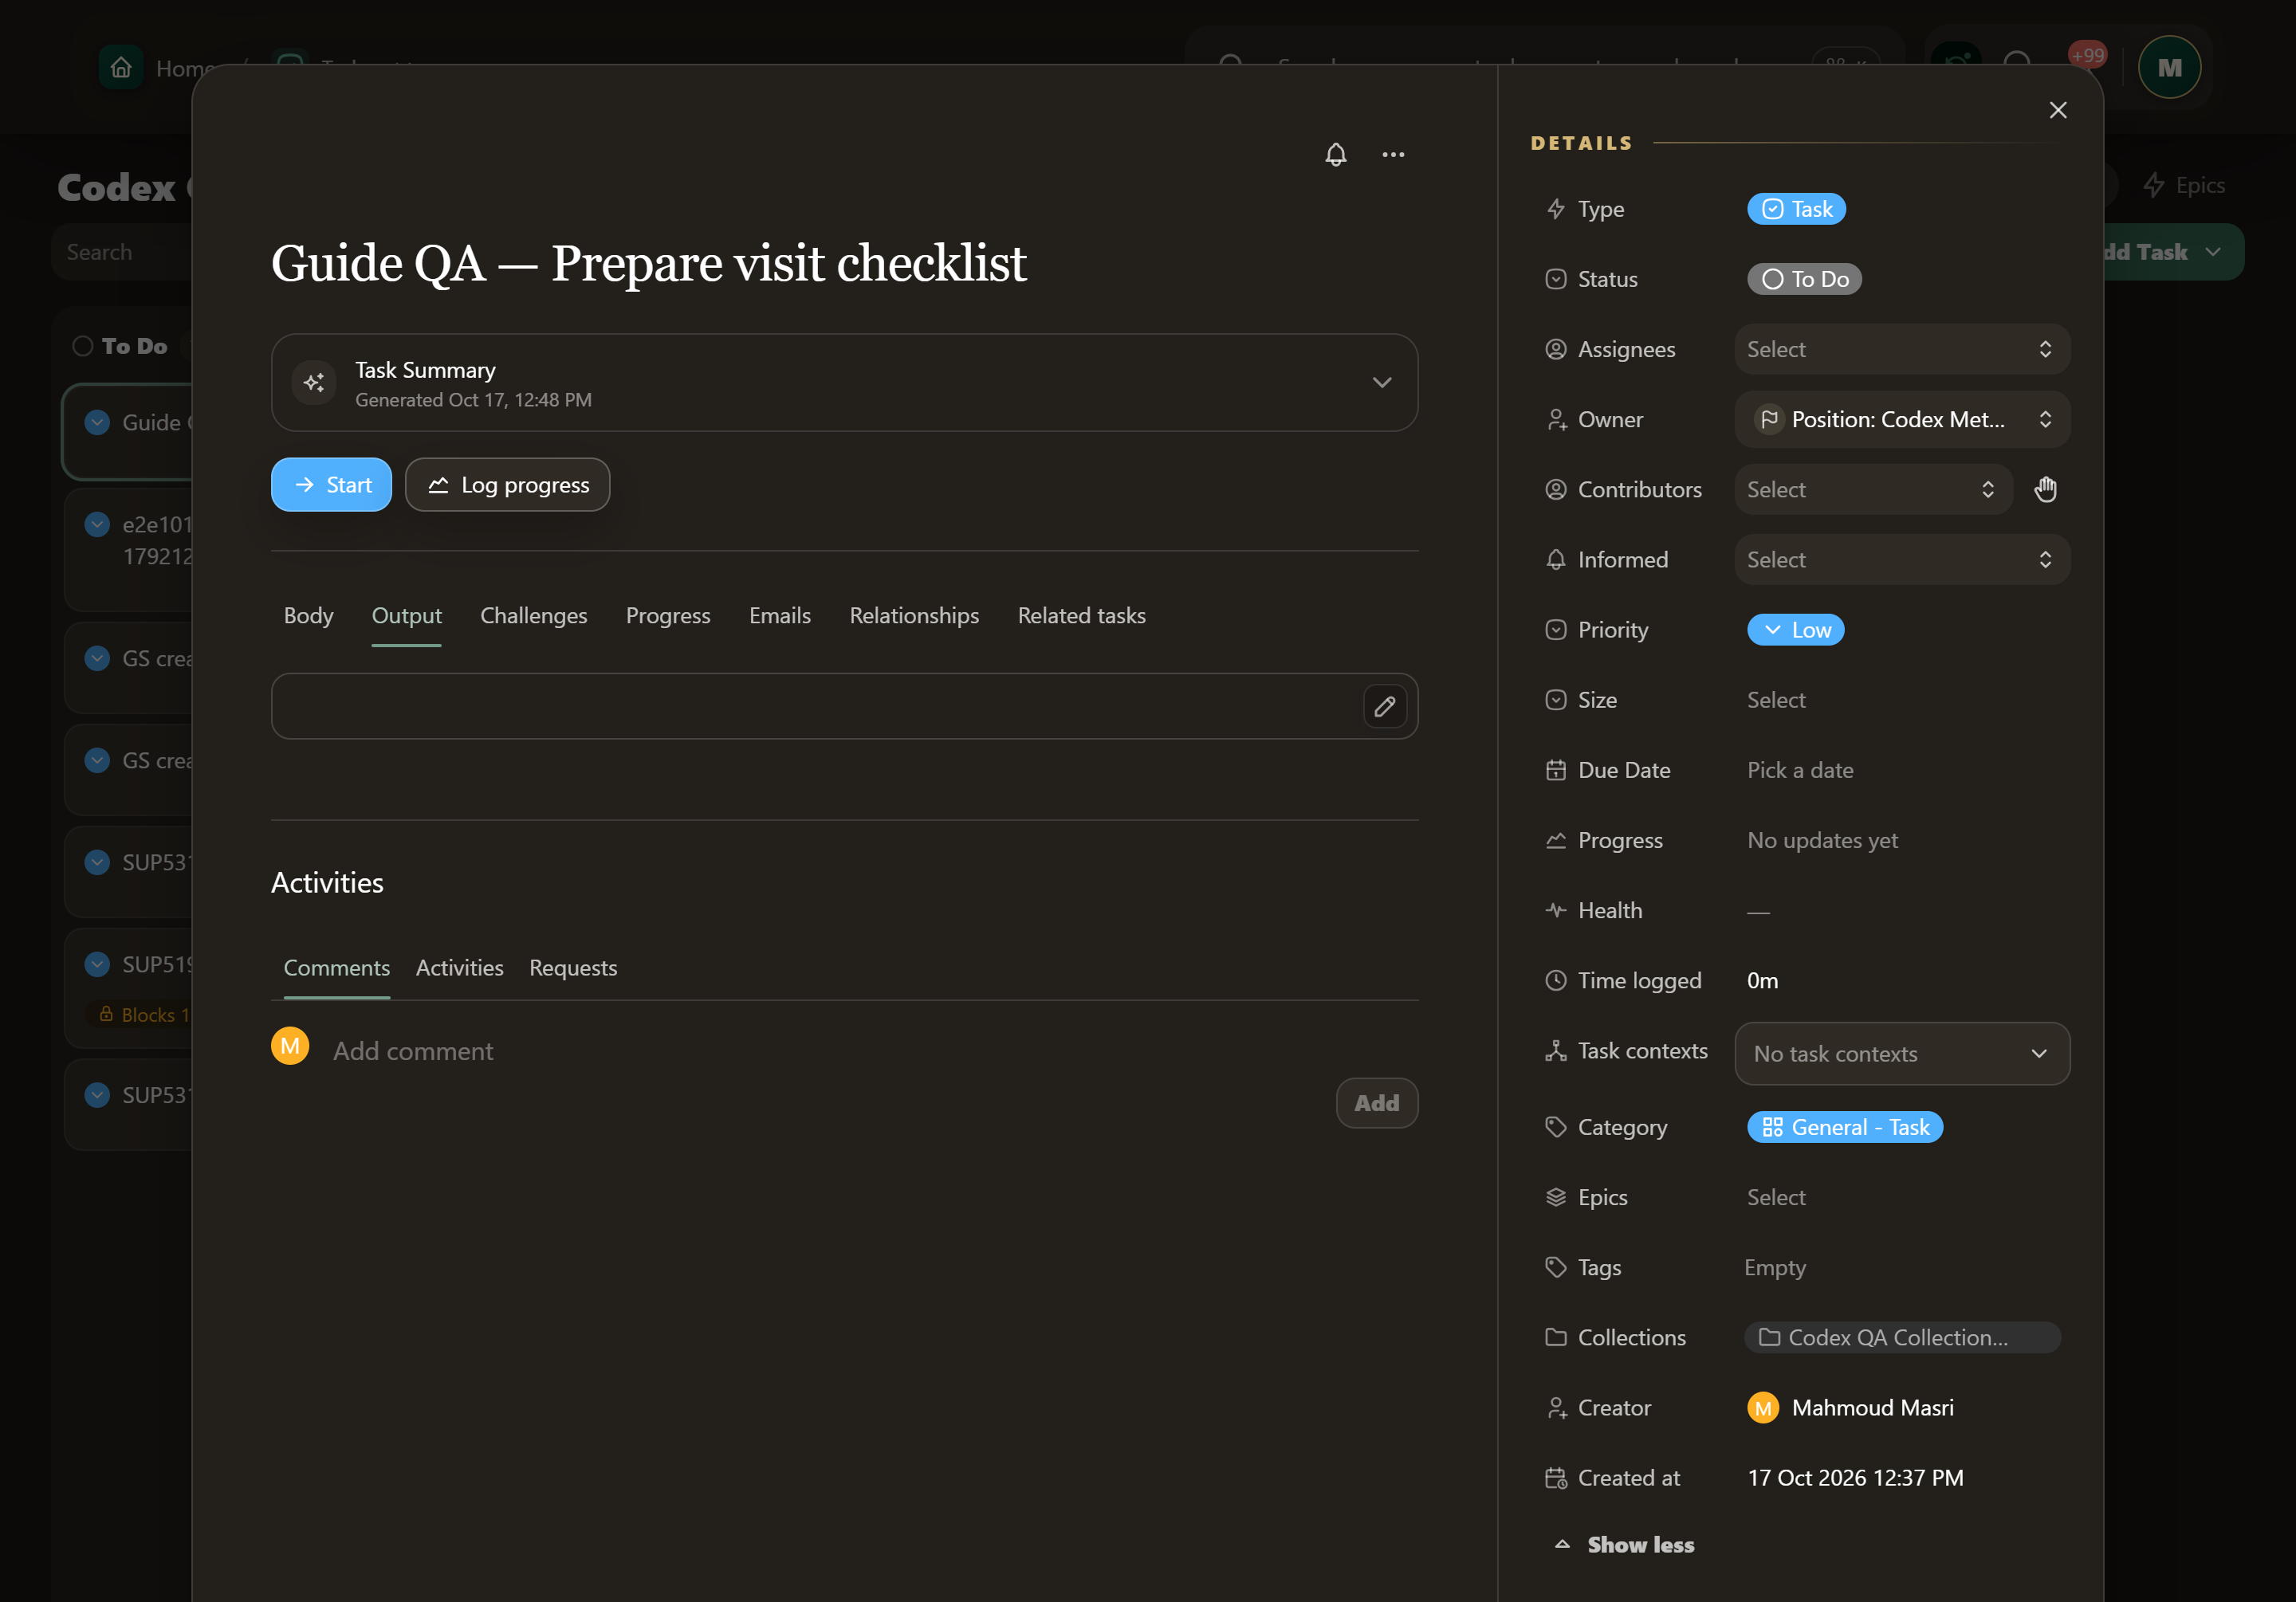
\includegraphics[width=0.95\linewidth,height=0.72\textheight,keepaspectratio]{figures/screens/ch04-output-en.png}
\caption{Output}
\label{fig:tasks-follow-up-output}
\shotnote{The Output tab is where you record what the work actually produced, after choosing the edit icon. This separates the description of what is required, in Body, from the delivered result. The tab stays empty, as in this test task, until the assignee records a result.}
\end{figure}

\begin{figure}[H]
\centering
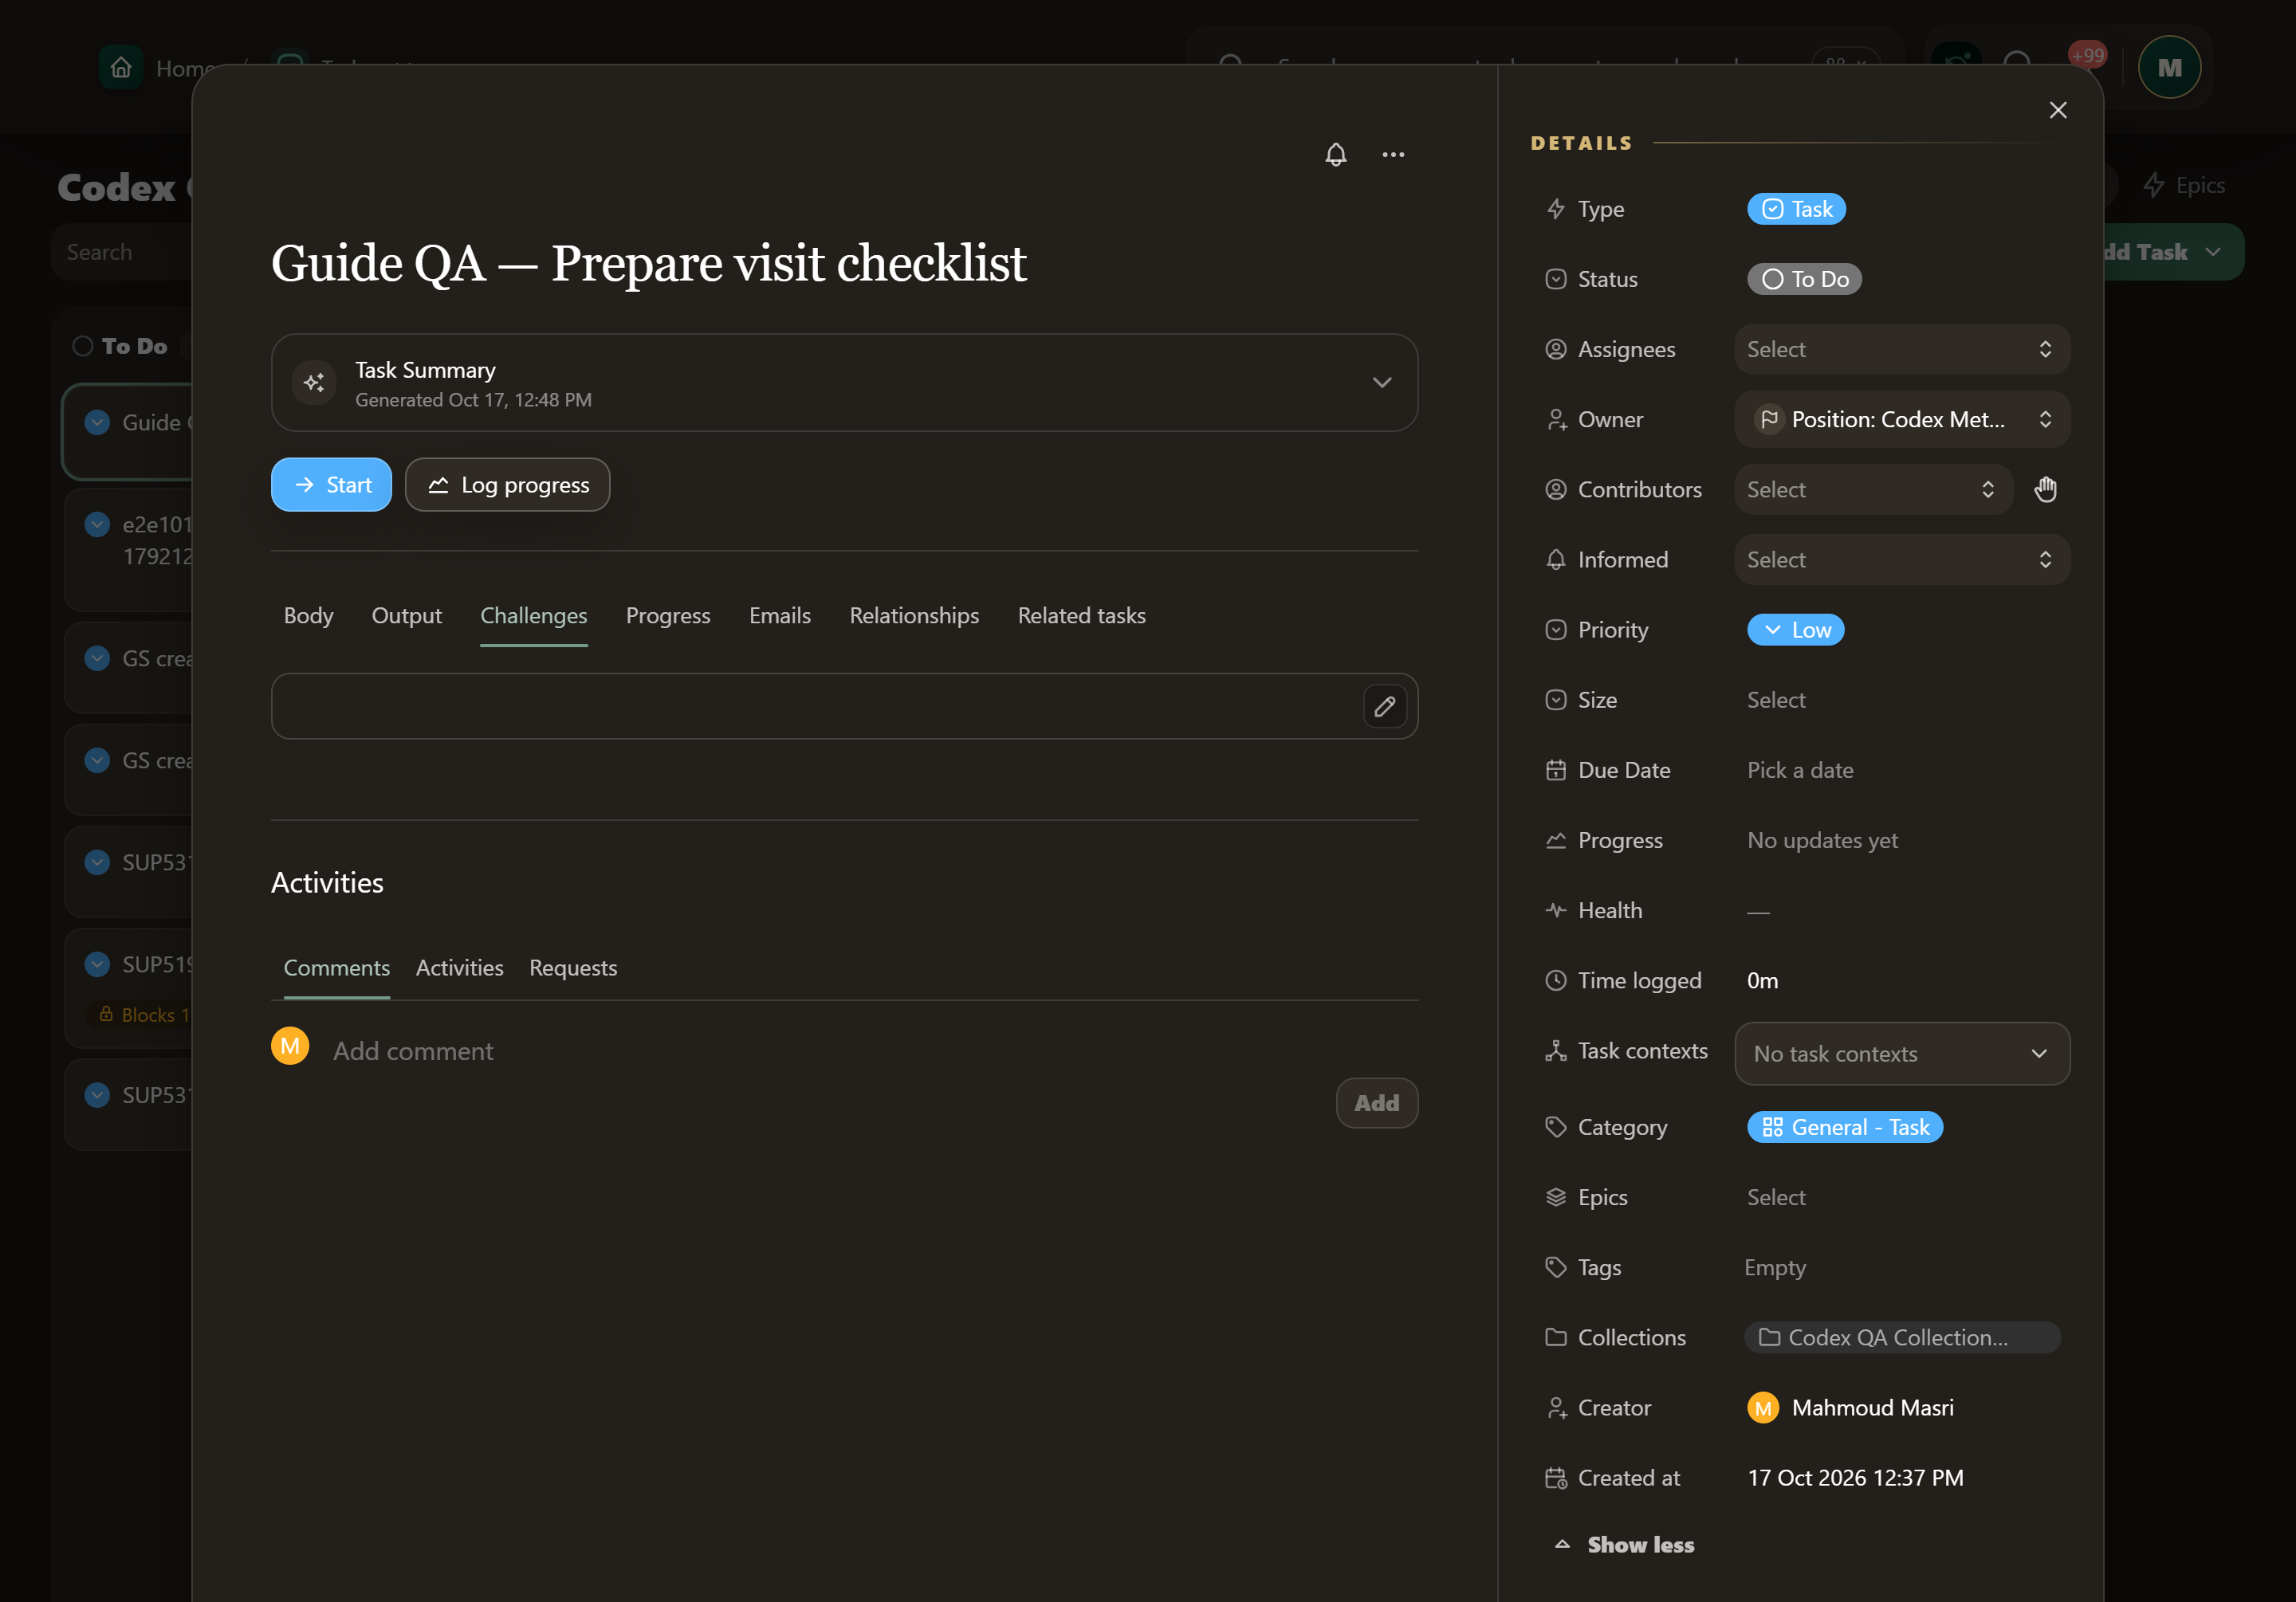
\includegraphics[width=0.95\linewidth,height=0.72\textheight,keepaspectratio]{figures/screens/ch04-challenges-en.png}
\caption{Challenges}
\label{fig:tasks-follow-up-challenges}
\shotnote{The Challenges tab is for obstacles that delay the work or need someone else’s decision; it is empty in this test task. Recording an obstacle here informs the team but does not change the task status automatically, so change status or ask for help separately.}
\end{figure}

\begin{figure}[H]
\centering
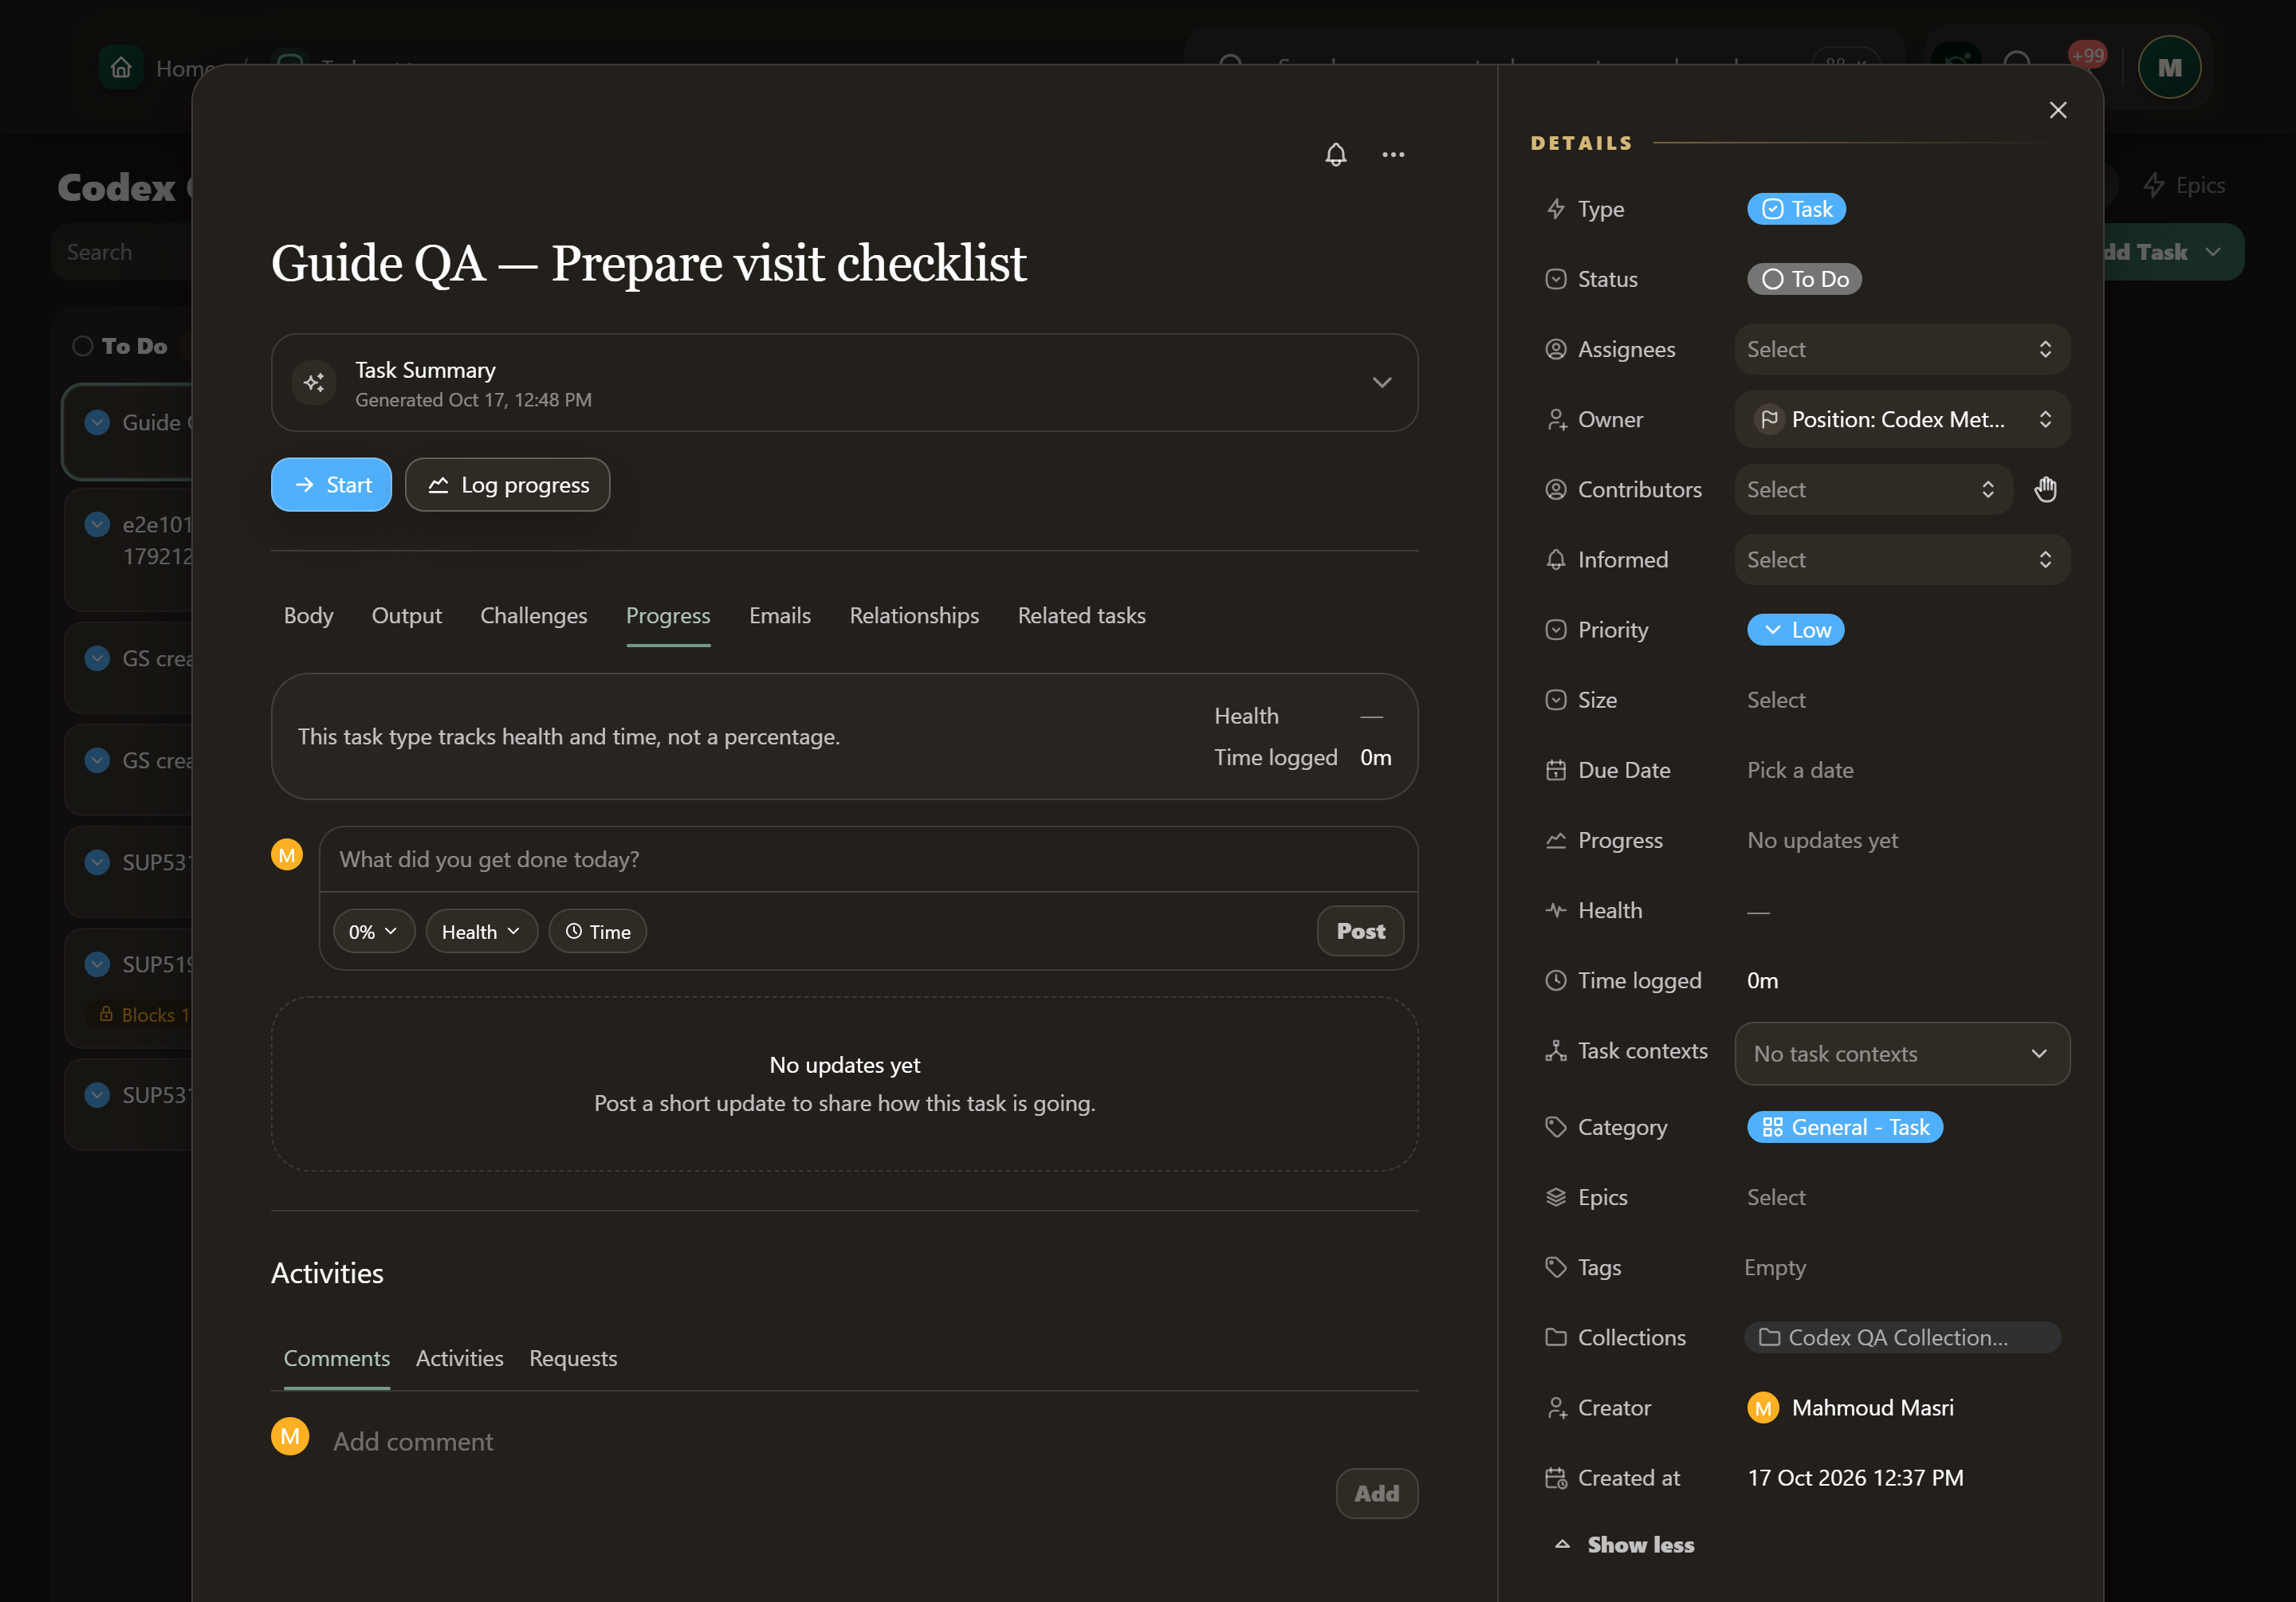
\includegraphics[width=0.95\linewidth,height=0.72\textheight,keepaspectratio]{figures/screens/ch04-progress-en.png}
\caption{Progress updates}
\label{fig:tasks-follow-up-progress}
\shotnote{The Progress tab collects short updates the team posts about the task: write in “What did you get done today?” and choose Post. The task type decides what is tracked; this task’s type, for instance, tracks status and time rather than a percentage. There are no updates on this test task yet.}
\end{figure}

\begin{figure}[H]
\centering
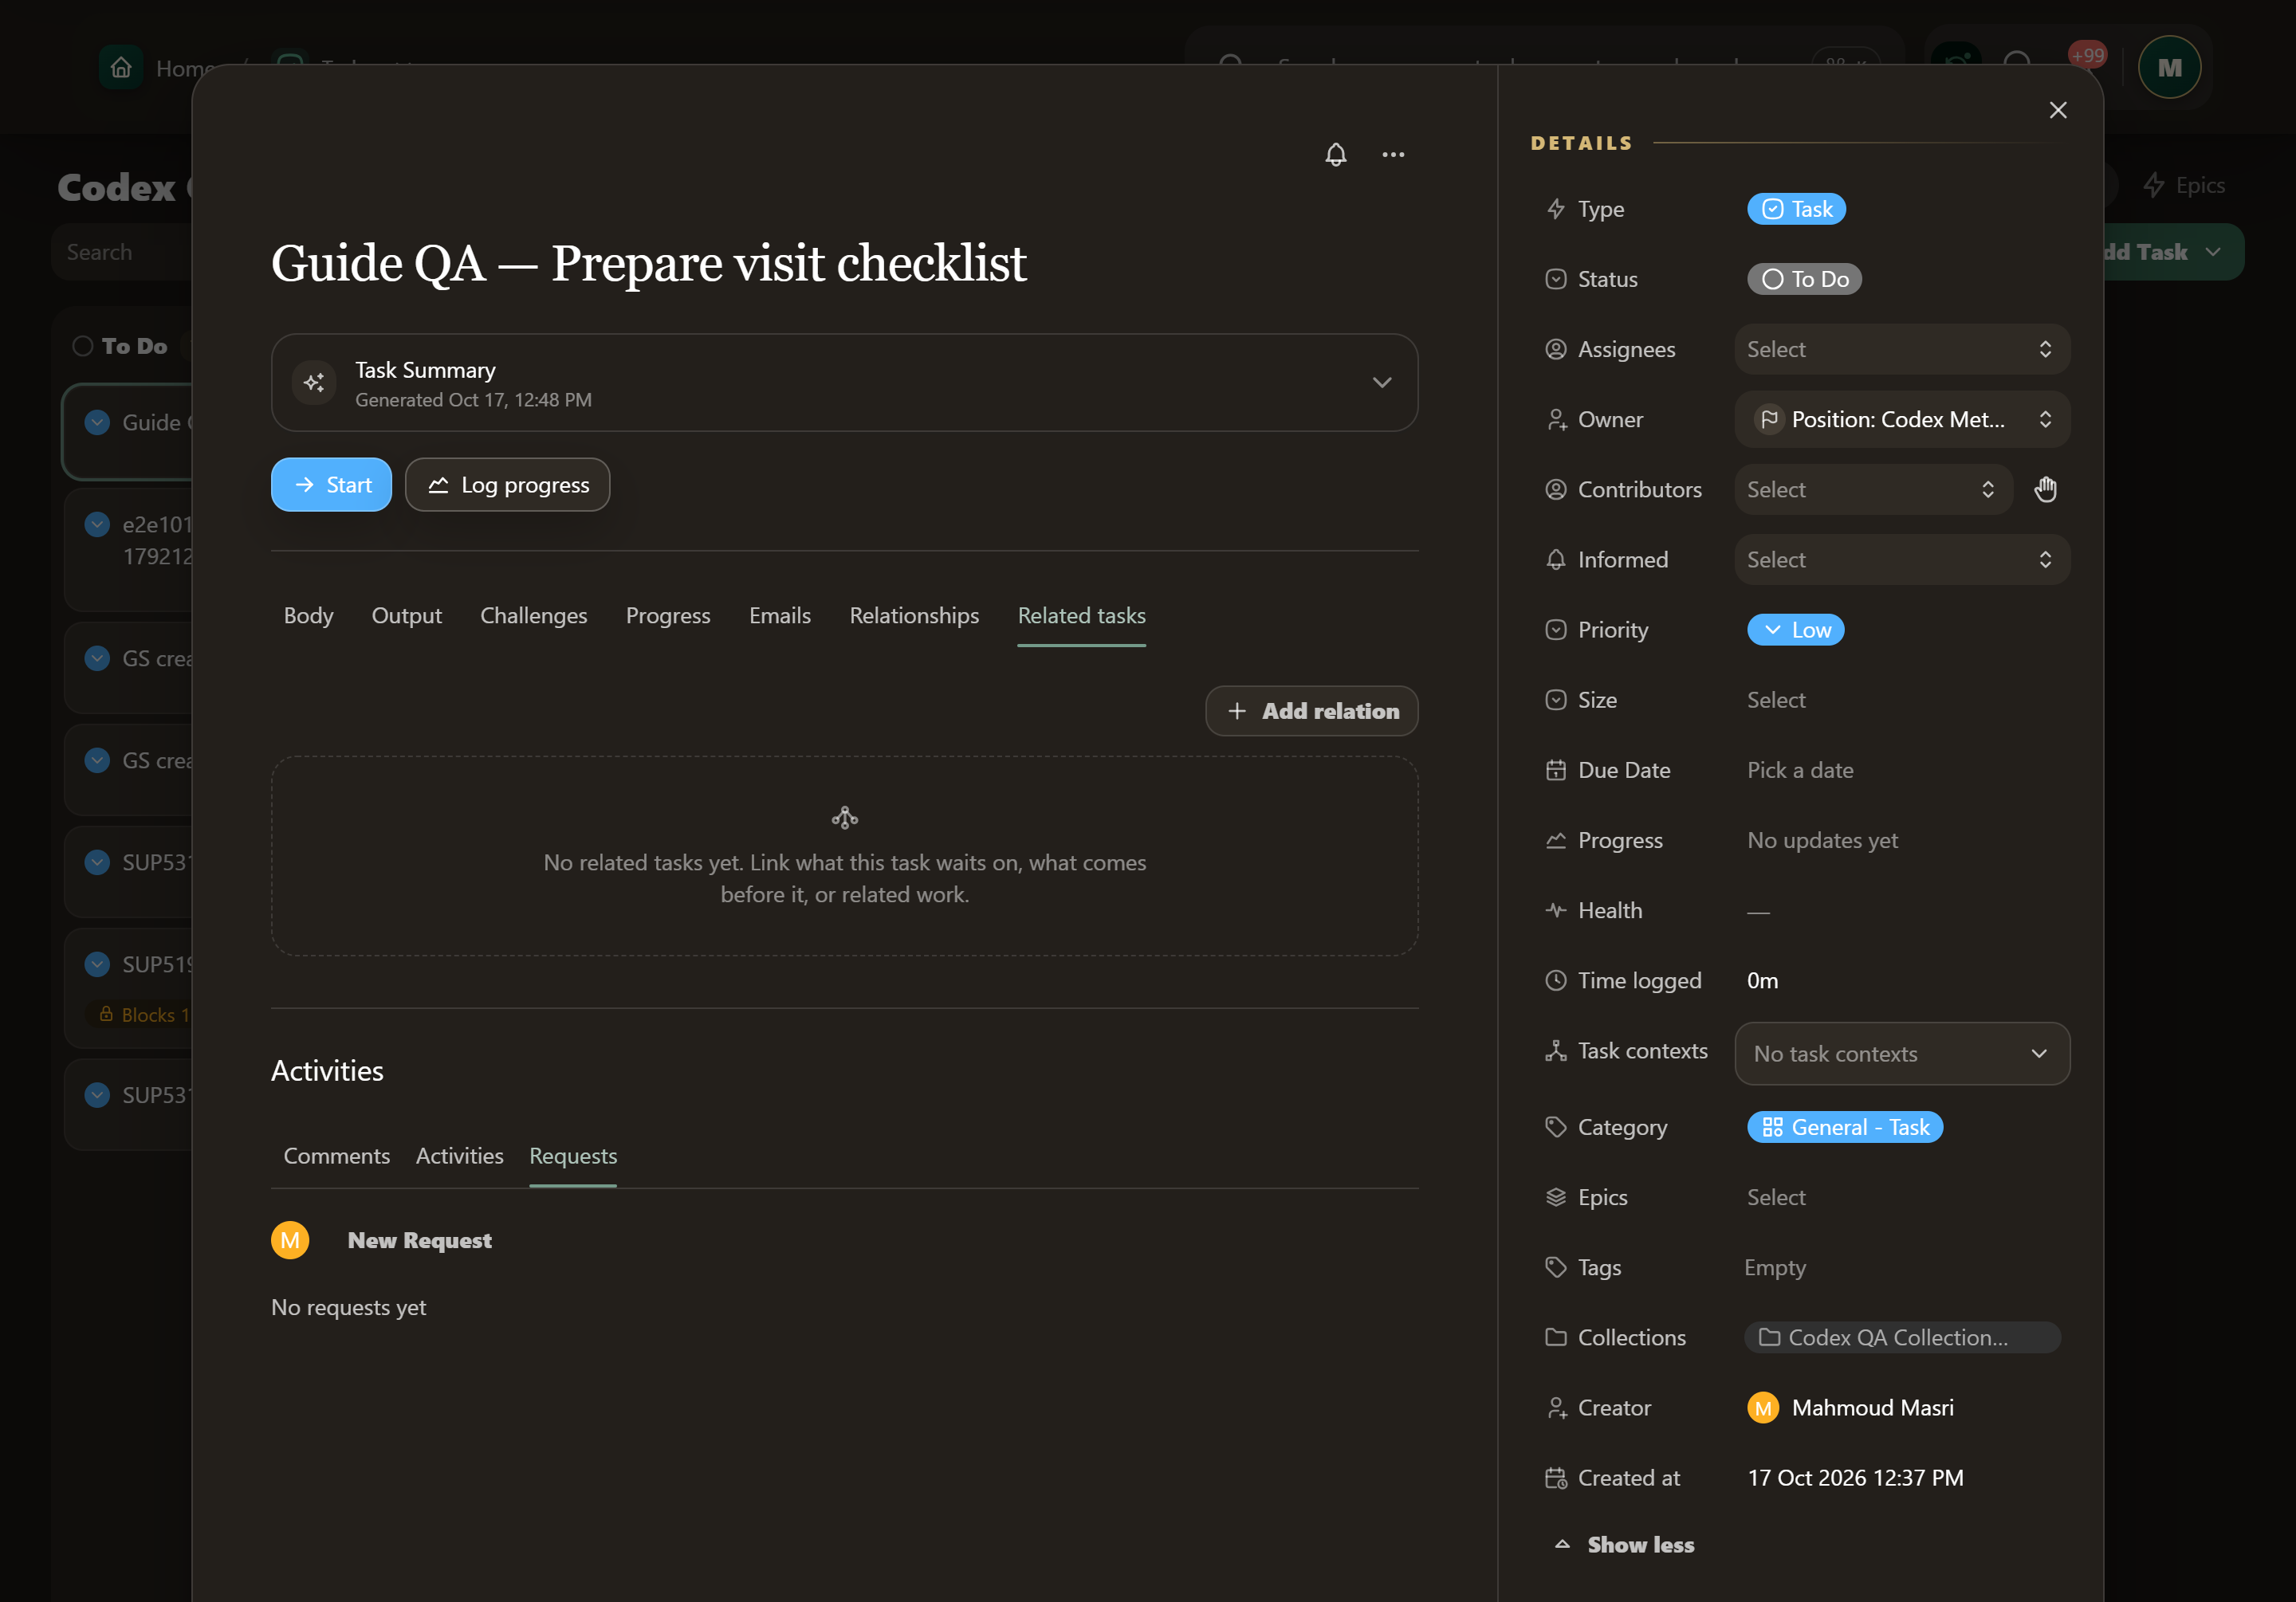
\includegraphics[width=0.95\linewidth,height=0.72\textheight,keepaspectratio]{figures/screens/ch04-requests-en.png}
\caption{Requests within a task}
\label{fig:tasks-follow-up-requests}
\shotnote{Requests let you ask another member for a specific action within the task record itself through New request, so the request and its response stay attached to the work instead of being lost in messages. Request status is separate from task status; this test task has no requests.}
\end{figure}

\begin{figure}[H]
\centering
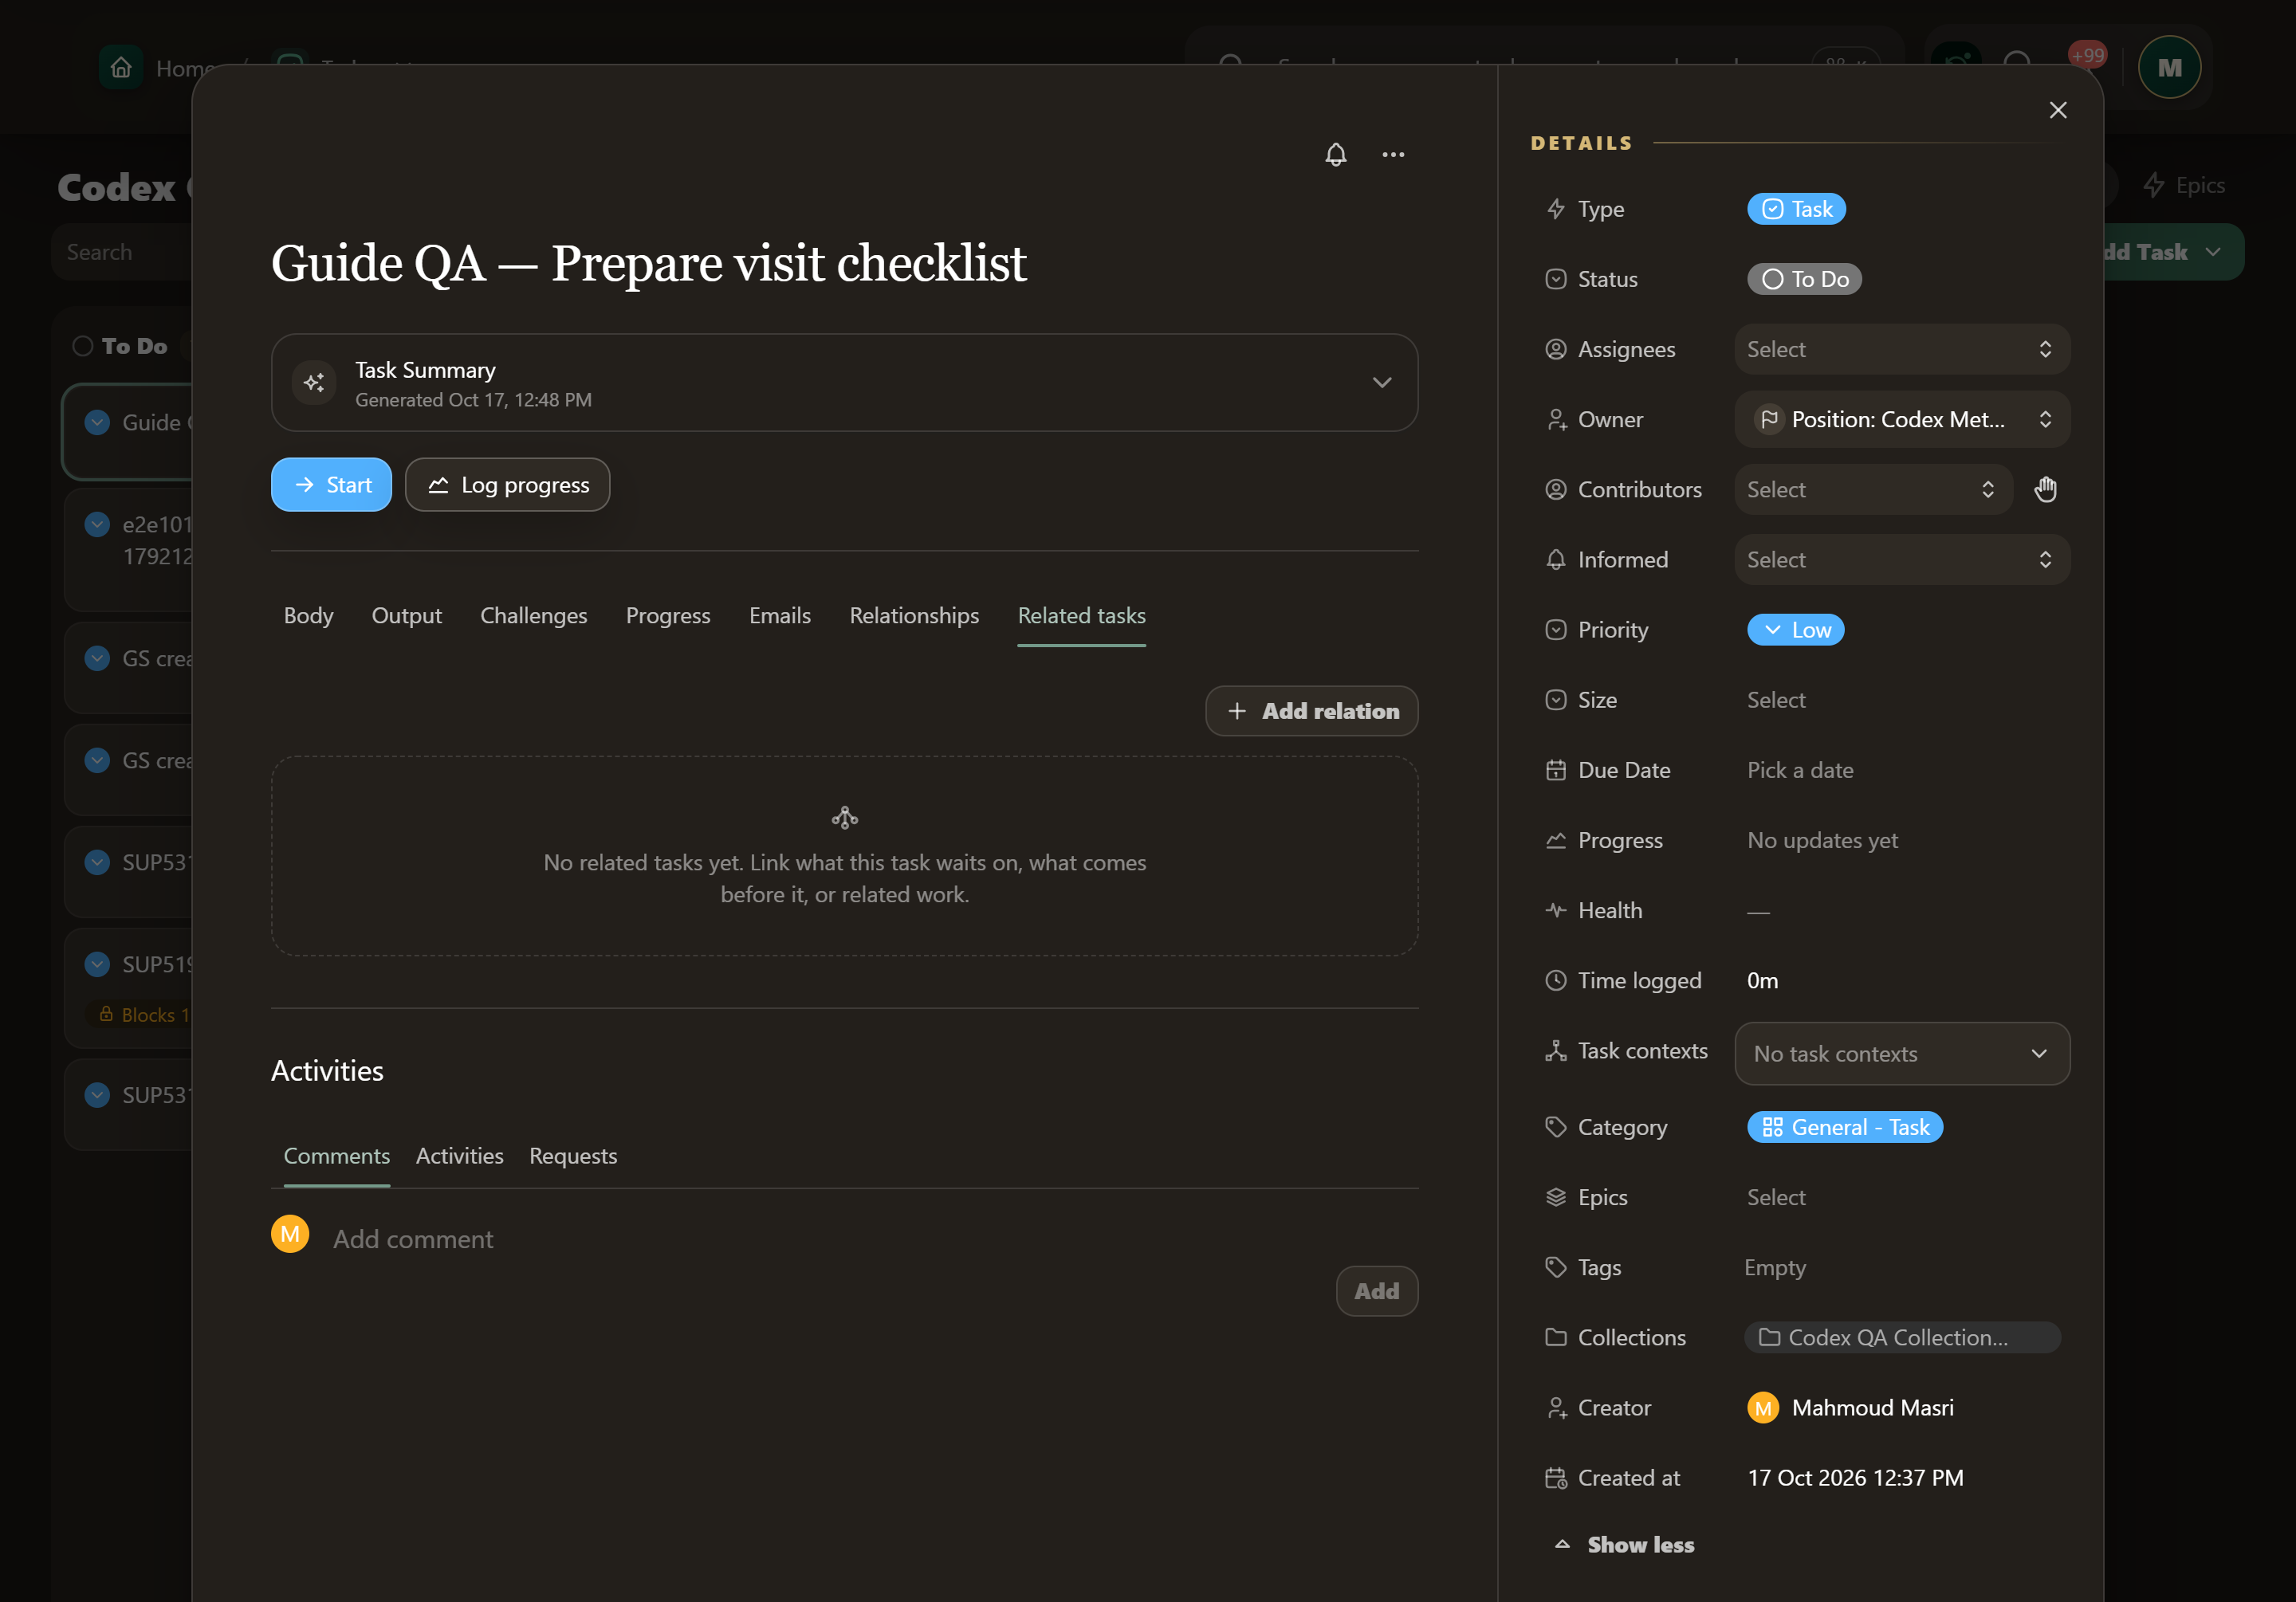
\includegraphics[width=0.95\linewidth,height=0.72\textheight,keepaspectratio]{figures/screens/ch04-comments-en.png}
\caption{Comments}
\label{fig:tasks-follow-up-comments}
\shotnote{Comments hold the team’s discussion of the task: type in Add comment and choose Add. A comment helps explain decisions and raise questions, but it does not change task status or replace recording the result in Output.}
\end{figure}

\begin{figure}[H]
\centering
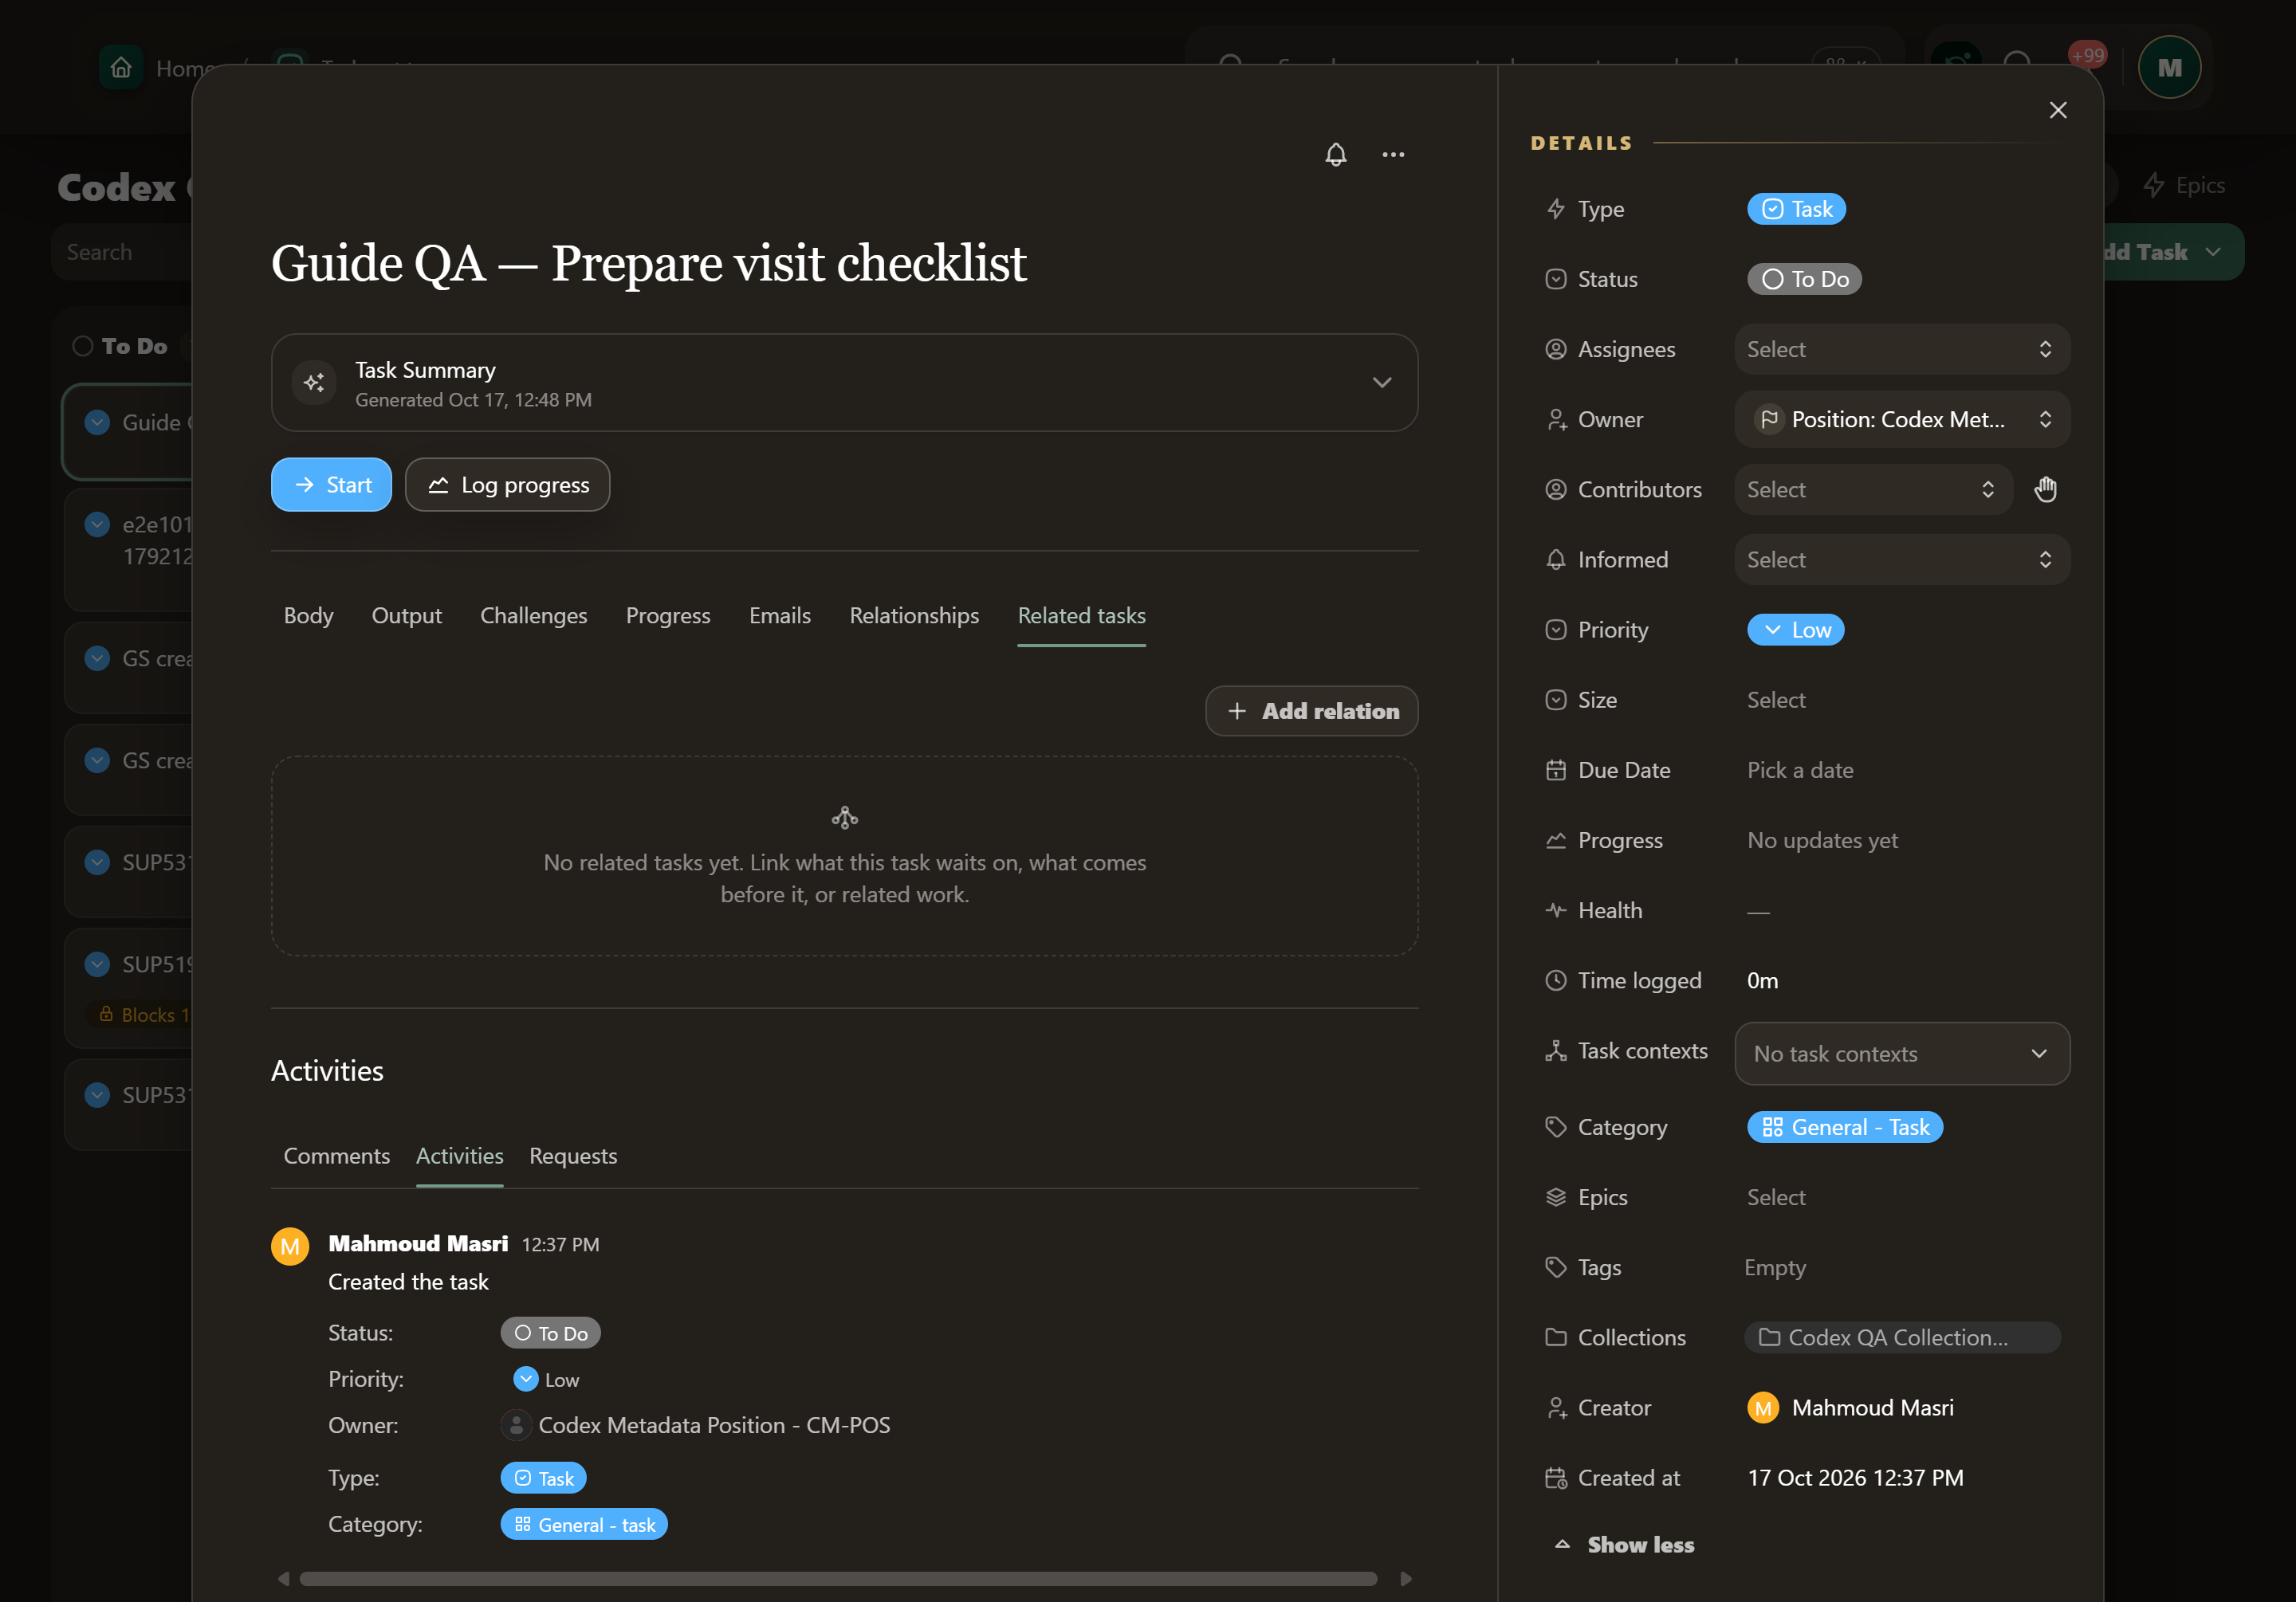
\includegraphics[width=0.95\linewidth,height=0.72\textheight,keepaspectratio]{figures/screens/ch04-activity-en.png}
\caption{Activity history}
\label{fig:tasks-follow-up-activity}
\shotnote{The Activities tab is a timeline of what happened to the task and who did it; here it shows the creation event with the initial status, owner and type. Owners consult it when asking about a change, while the work result belongs in Output, not here.}
\end{figure}

\begin{table}[H]
\centering
\caption{What can you record or do?}
\label{tab:tasks-follow-up-data}
\begin{tabularx}{\linewidth}{R{3.6cm} Y}
\rcHeaderRow
\thh{Section} & \thh{Content and action}\\
Body, output and challenges & Execution context, result and obstacles. The content editor supports files where attachment controls are available.\\
Progress & Dated updates, completion percentage, health, time, next steps and blockers, depending on type configuration.\\
Comments and activities & Work discussion and change history. Follow or unfollow controls your task subscription.\\
Requests and summary & Request contribution or a response from another member; request status is separate from task status. Review an assisted summary against the record.\\
\end{tabularx}
\end{table}

\begin{figure}[H]
\centering
\begin{tikzpicture}[node distance=0.5cm]
\node[stepBox] (a) {\RL{Record result}};
\node[stepBox,below=of a] (b) {\RL{Resolve obstacle}};
\node[stepBox,below=of b] (c) {\RL{Review status}};
\draw[flowsTo] (a) -- (b);
\draw[flowsTo] (b) -- (c);
\end{tikzpicture}
\rclegend
\caption{Steps to follow}
\label{fig:tasks-follow-up-flow}
\shotnote{The diagram shows the follow-up order: record the result first so it is clear what was achieved, resolve any obstacle, then review the status and choose the right transition. Changing status before resolving an obstacle gives the team an inaccurate picture of the work.}
\end{figure}

\subsection{Steps and verification}
\begin{enumerate}
\item Open Output, edit the result and save. Use Challenges similarly when there is an obstacle.
\item If Log progress is available, open it, complete the update and required fields, then save. Confirm it appears in Progress.
\item For discussion, write a comment and choose Add. For an action request, open Requests, choose another member and a precise request, then send and track it.
\item After reviewing the result, use an available status transition. If refused, check blockers and required relationships.
\end{enumerate}

\textbf{Check and recovery:} Reopen to verify result, update and status. Task completion is not a formal approval or a signature on another record.

\clearpage
\section{Relationships and linked records}
\label{sec:tasks-feature-relationships}

Relationships connect a task to its source, evidence or another task. Choose the relationship meaning before selecting the record so colleagues understand the link.

\textbf{Where and who:} Task → Relationships, Related tasks or Emails. For an authorized editor.

\begin{rcnote}[Example: Horizon]
Sarah links checklist preparation to the visit record and identifies address confirmation as a prerequisite. Omar can see what he is waiting for and where the source is.
\end{rcnote}

\begin{figure}[H]
\centering
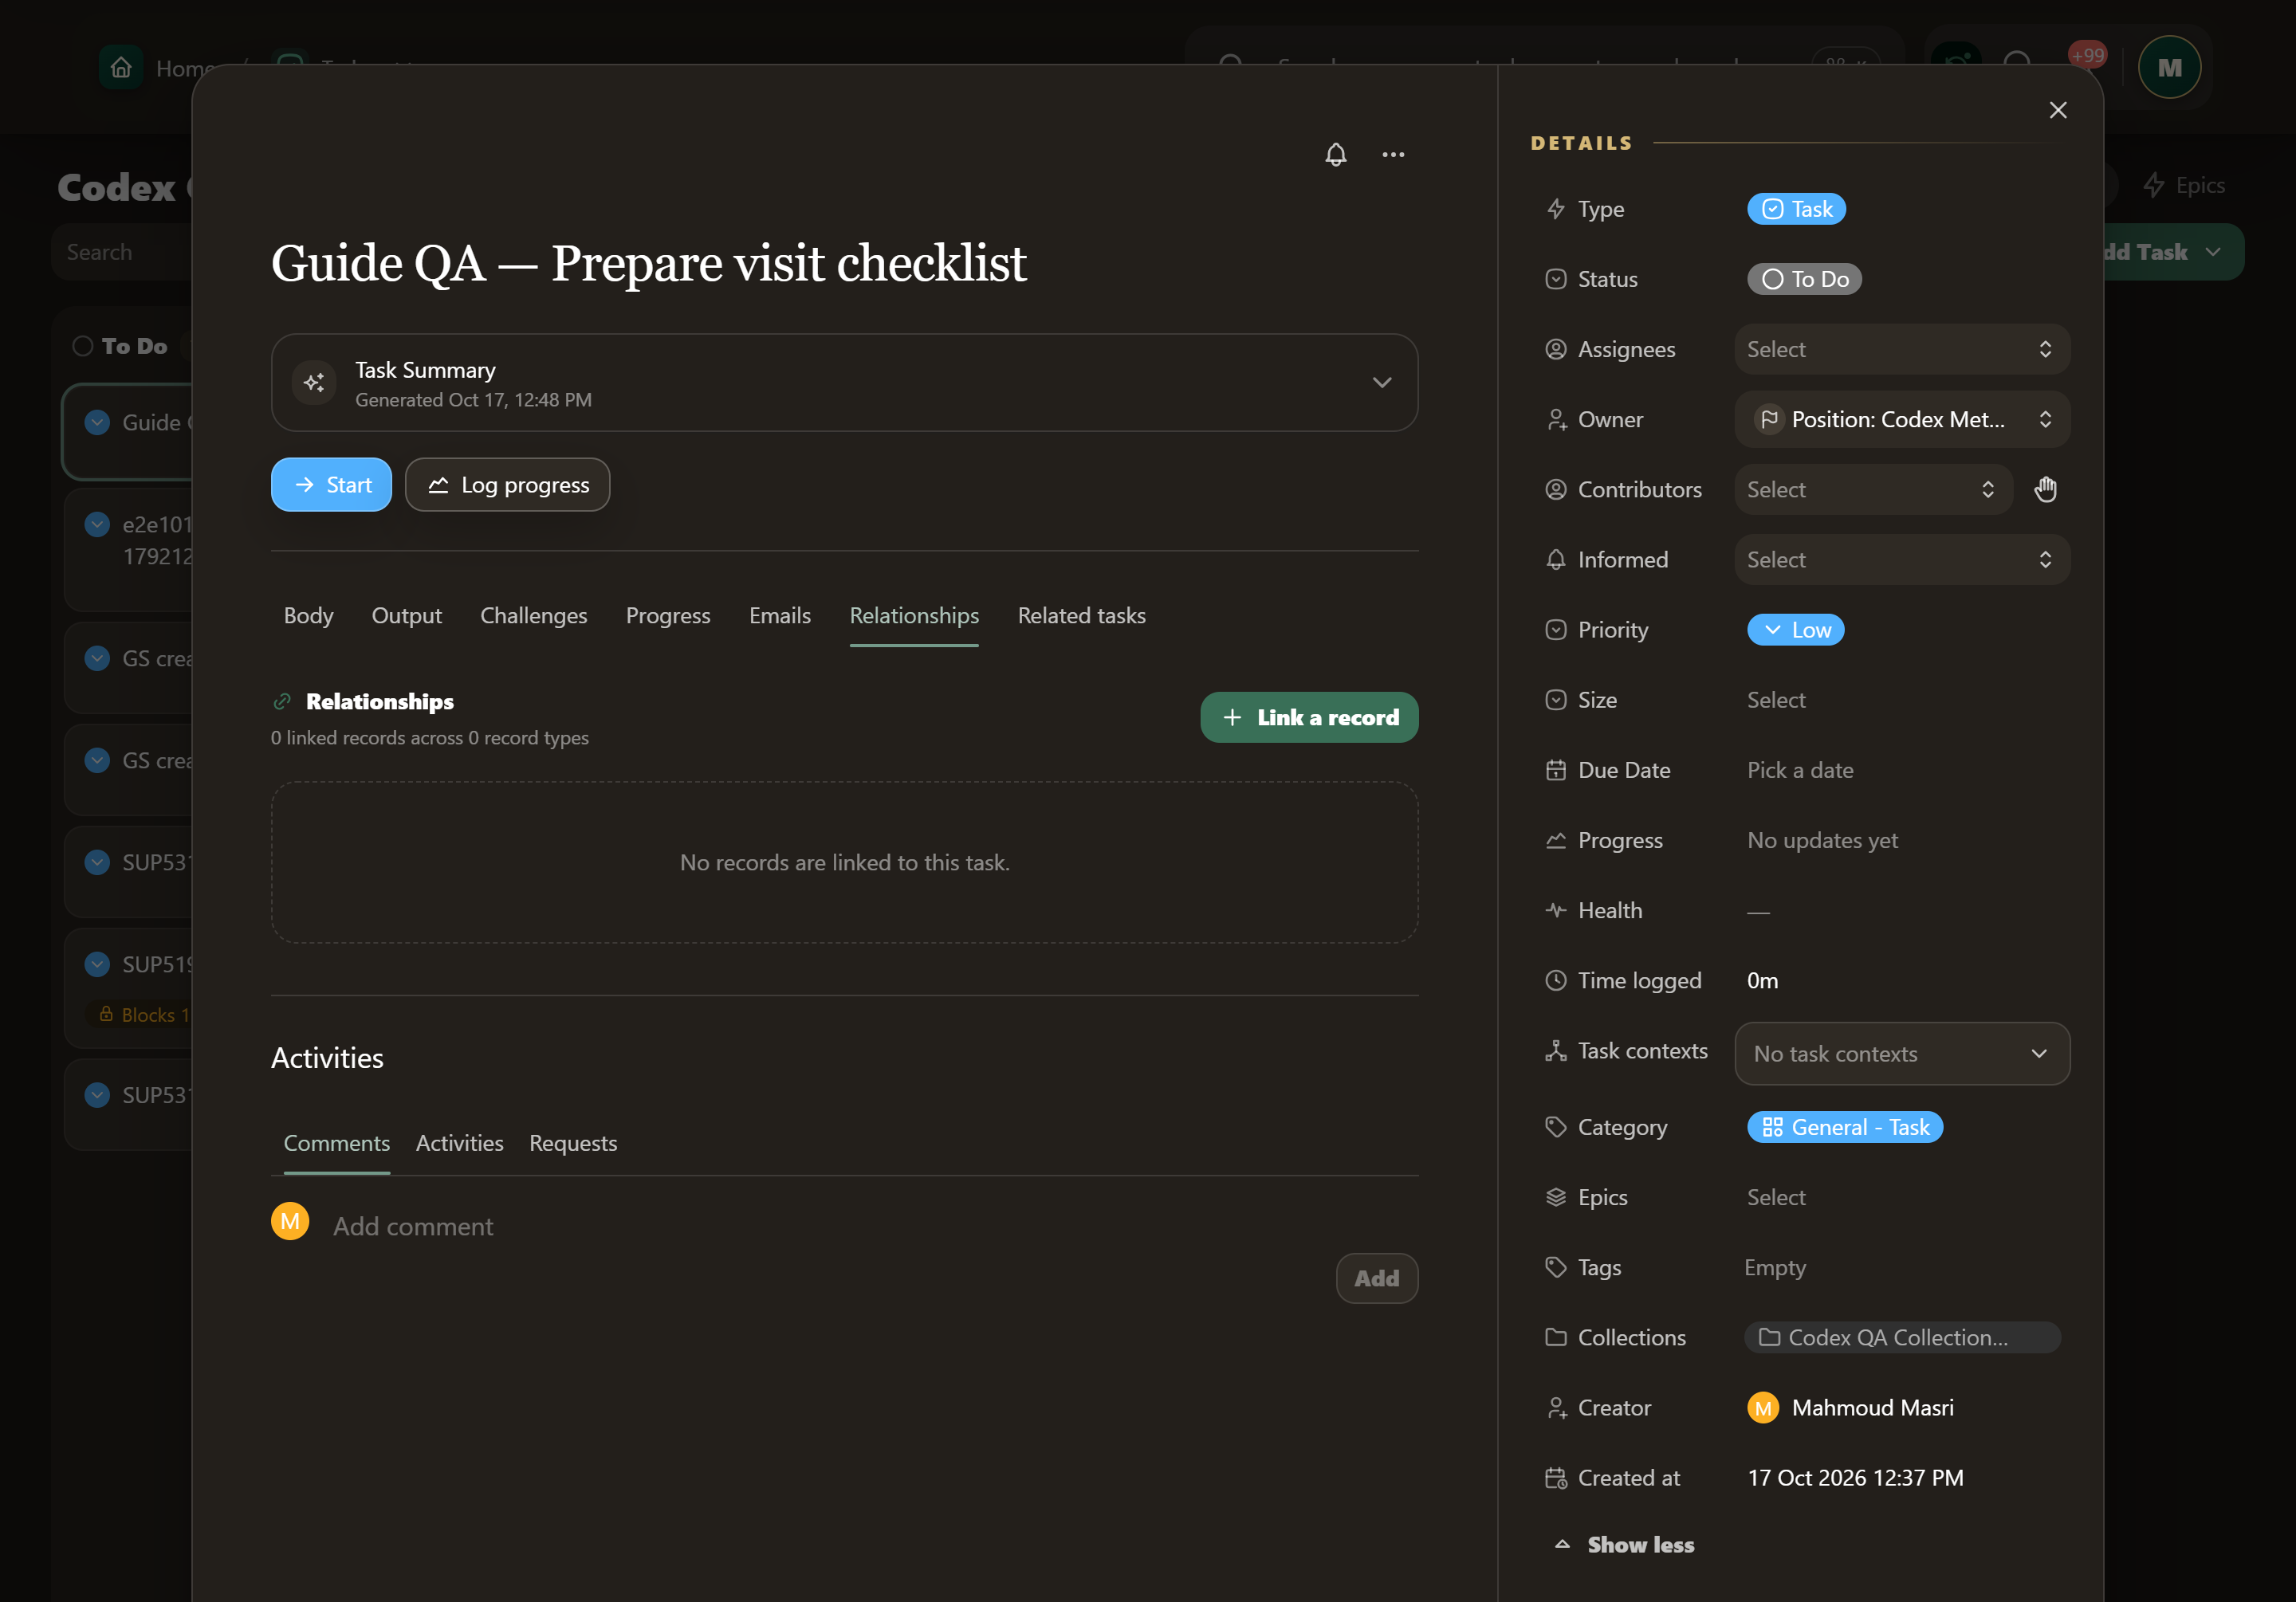
\includegraphics[width=0.95\linewidth,height=0.72\textheight,keepaspectratio]{figures/screens/ch04-records-en.png}
\caption{Record relationships}
\label{fig:tasks-relationships-records}
\shotnote{The Relationships tab links the task to records outside Tasks, such as a record that is its subject or proves its completion, and shows how many are linked. Linking starts with Link record and a relationship meaning chosen from the allowed types. A link does not grant record access to someone without it; this test task has none.}
\end{figure}

\begin{figure}[H]
\centering
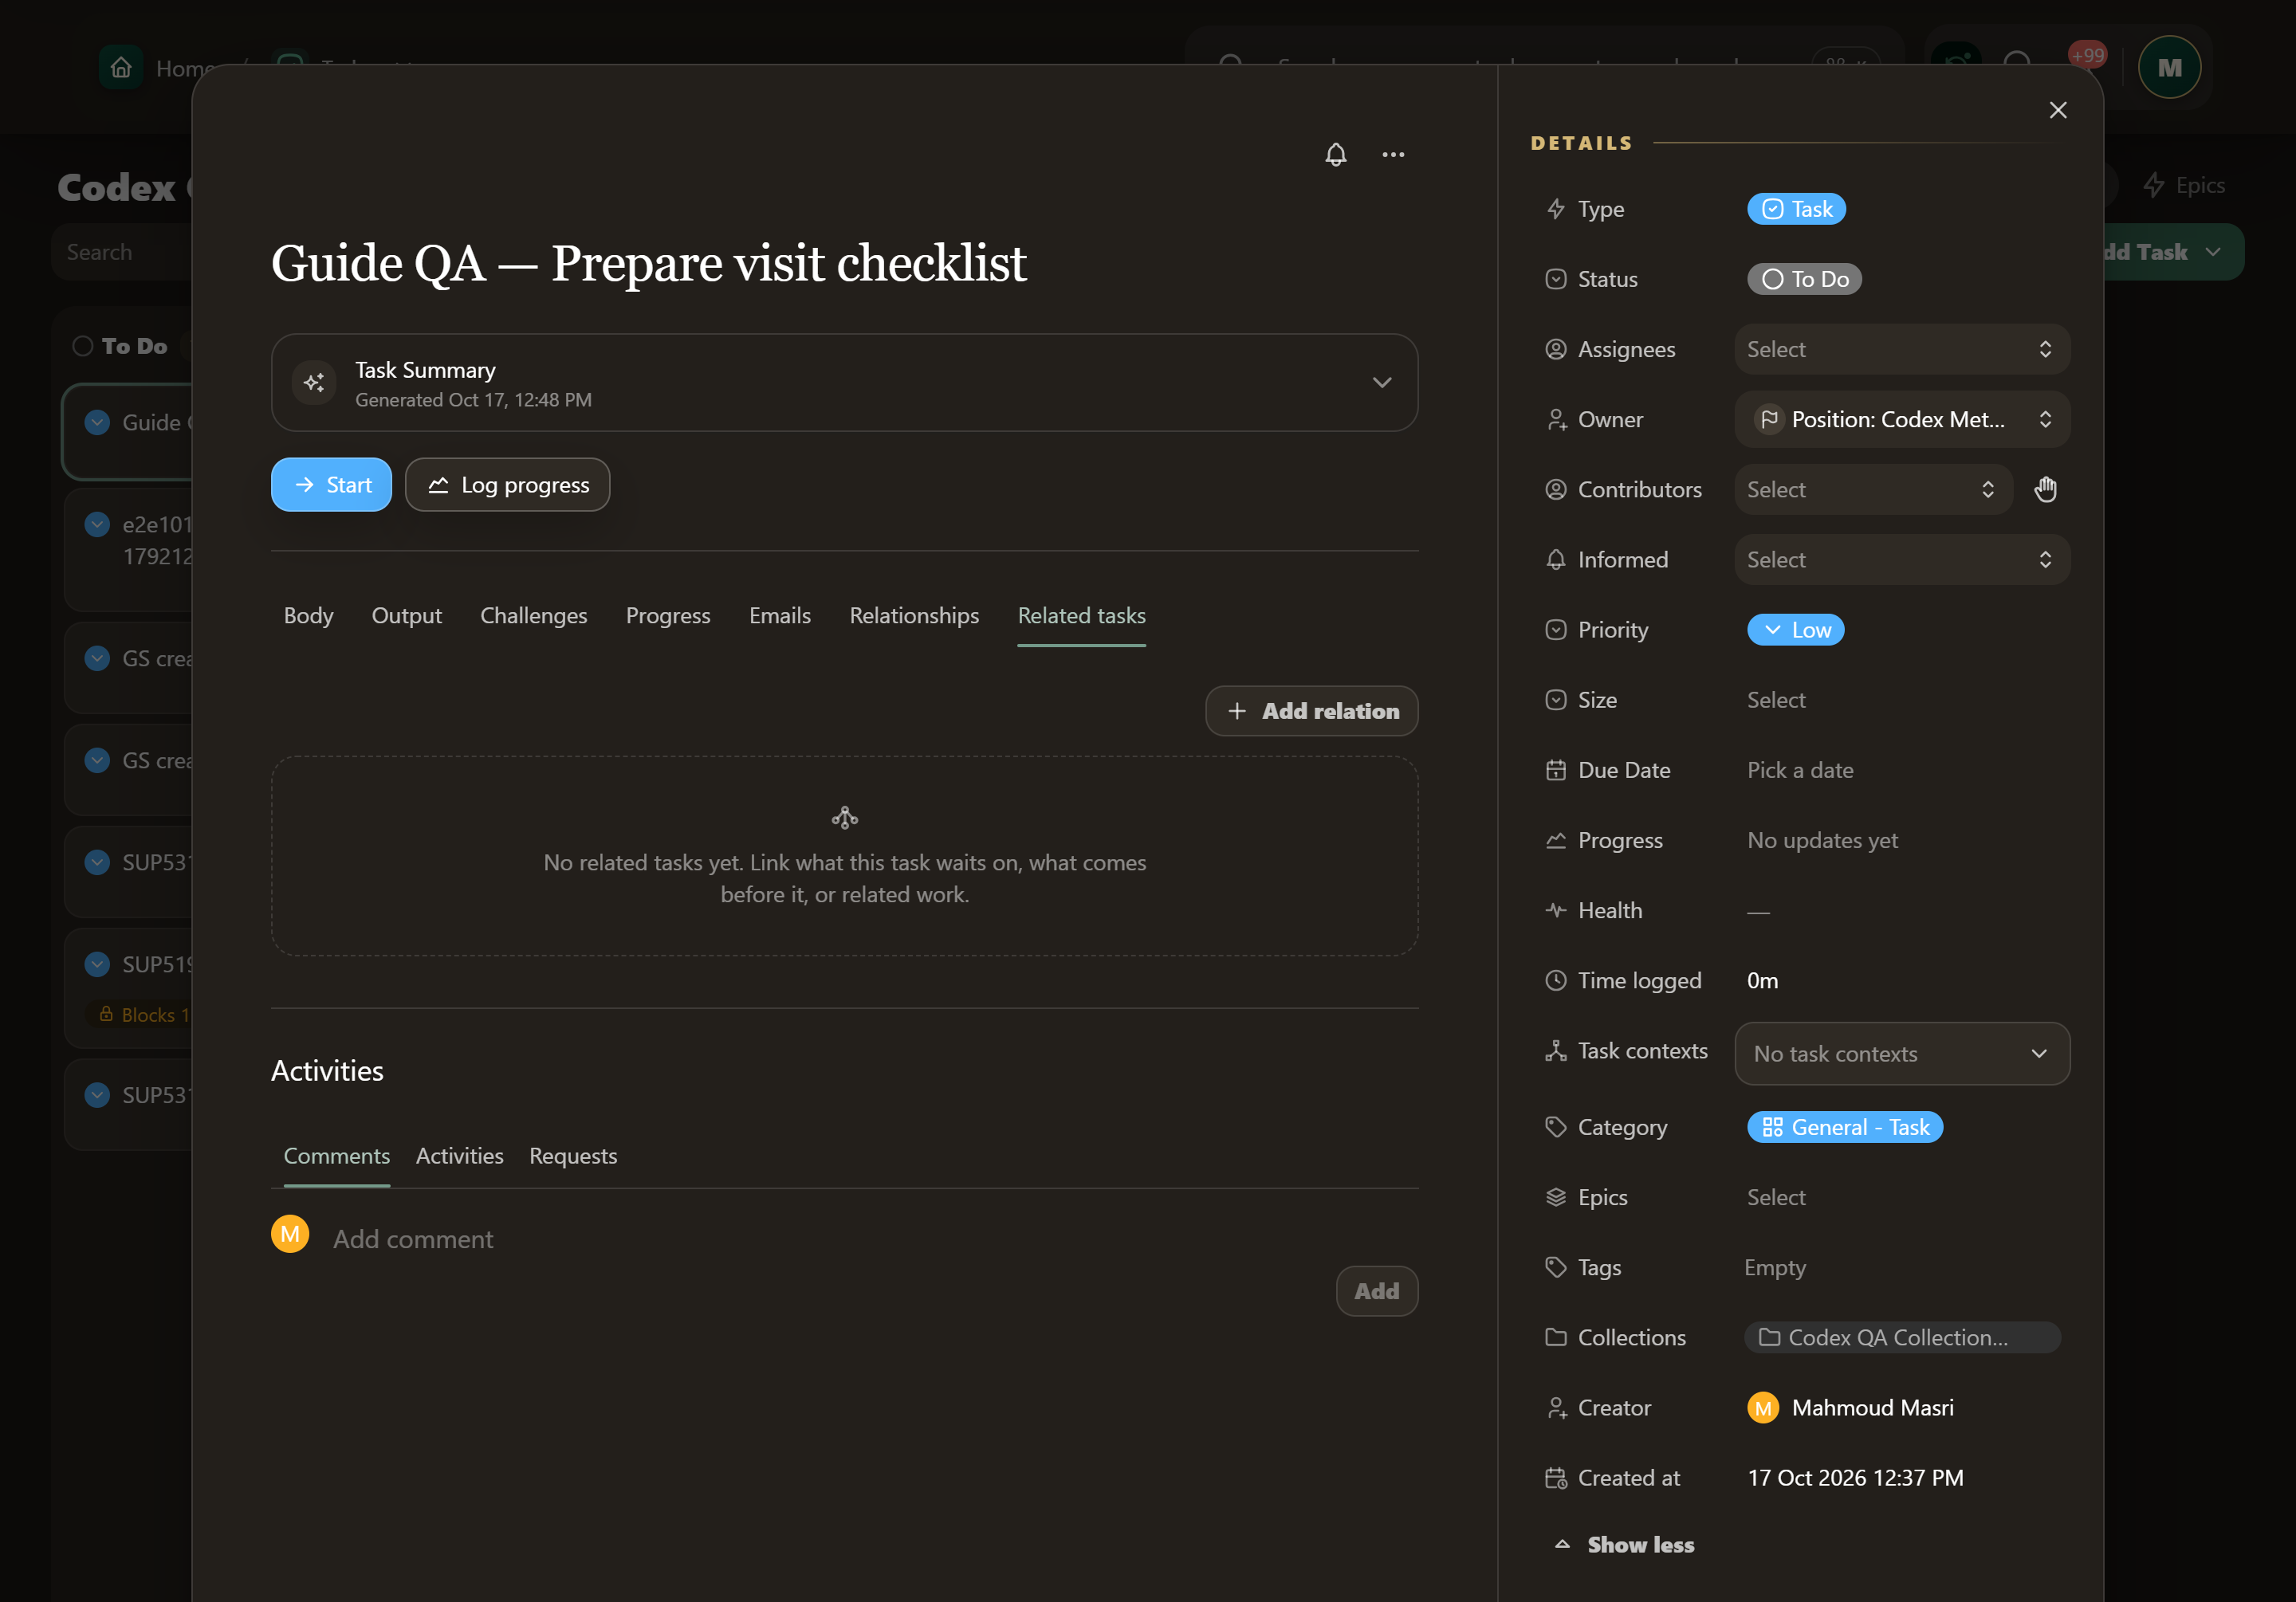
\includegraphics[width=0.95\linewidth,height=0.72\textheight,keepaspectratio]{figures/screens/ch04-relations-en.png}
\caption{Related tasks}
\label{fig:tasks-relationships-relations}
\shotnote{The Related tasks tab shows how the task connects to other tasks: what it waits for, what precedes it and what relates to it; links are added with Add relation. Some of these relations affect work order, so check a blocking relation’s direction before saving. This test task has no relations yet.}
\end{figure}

\begin{figure}[H]
\centering
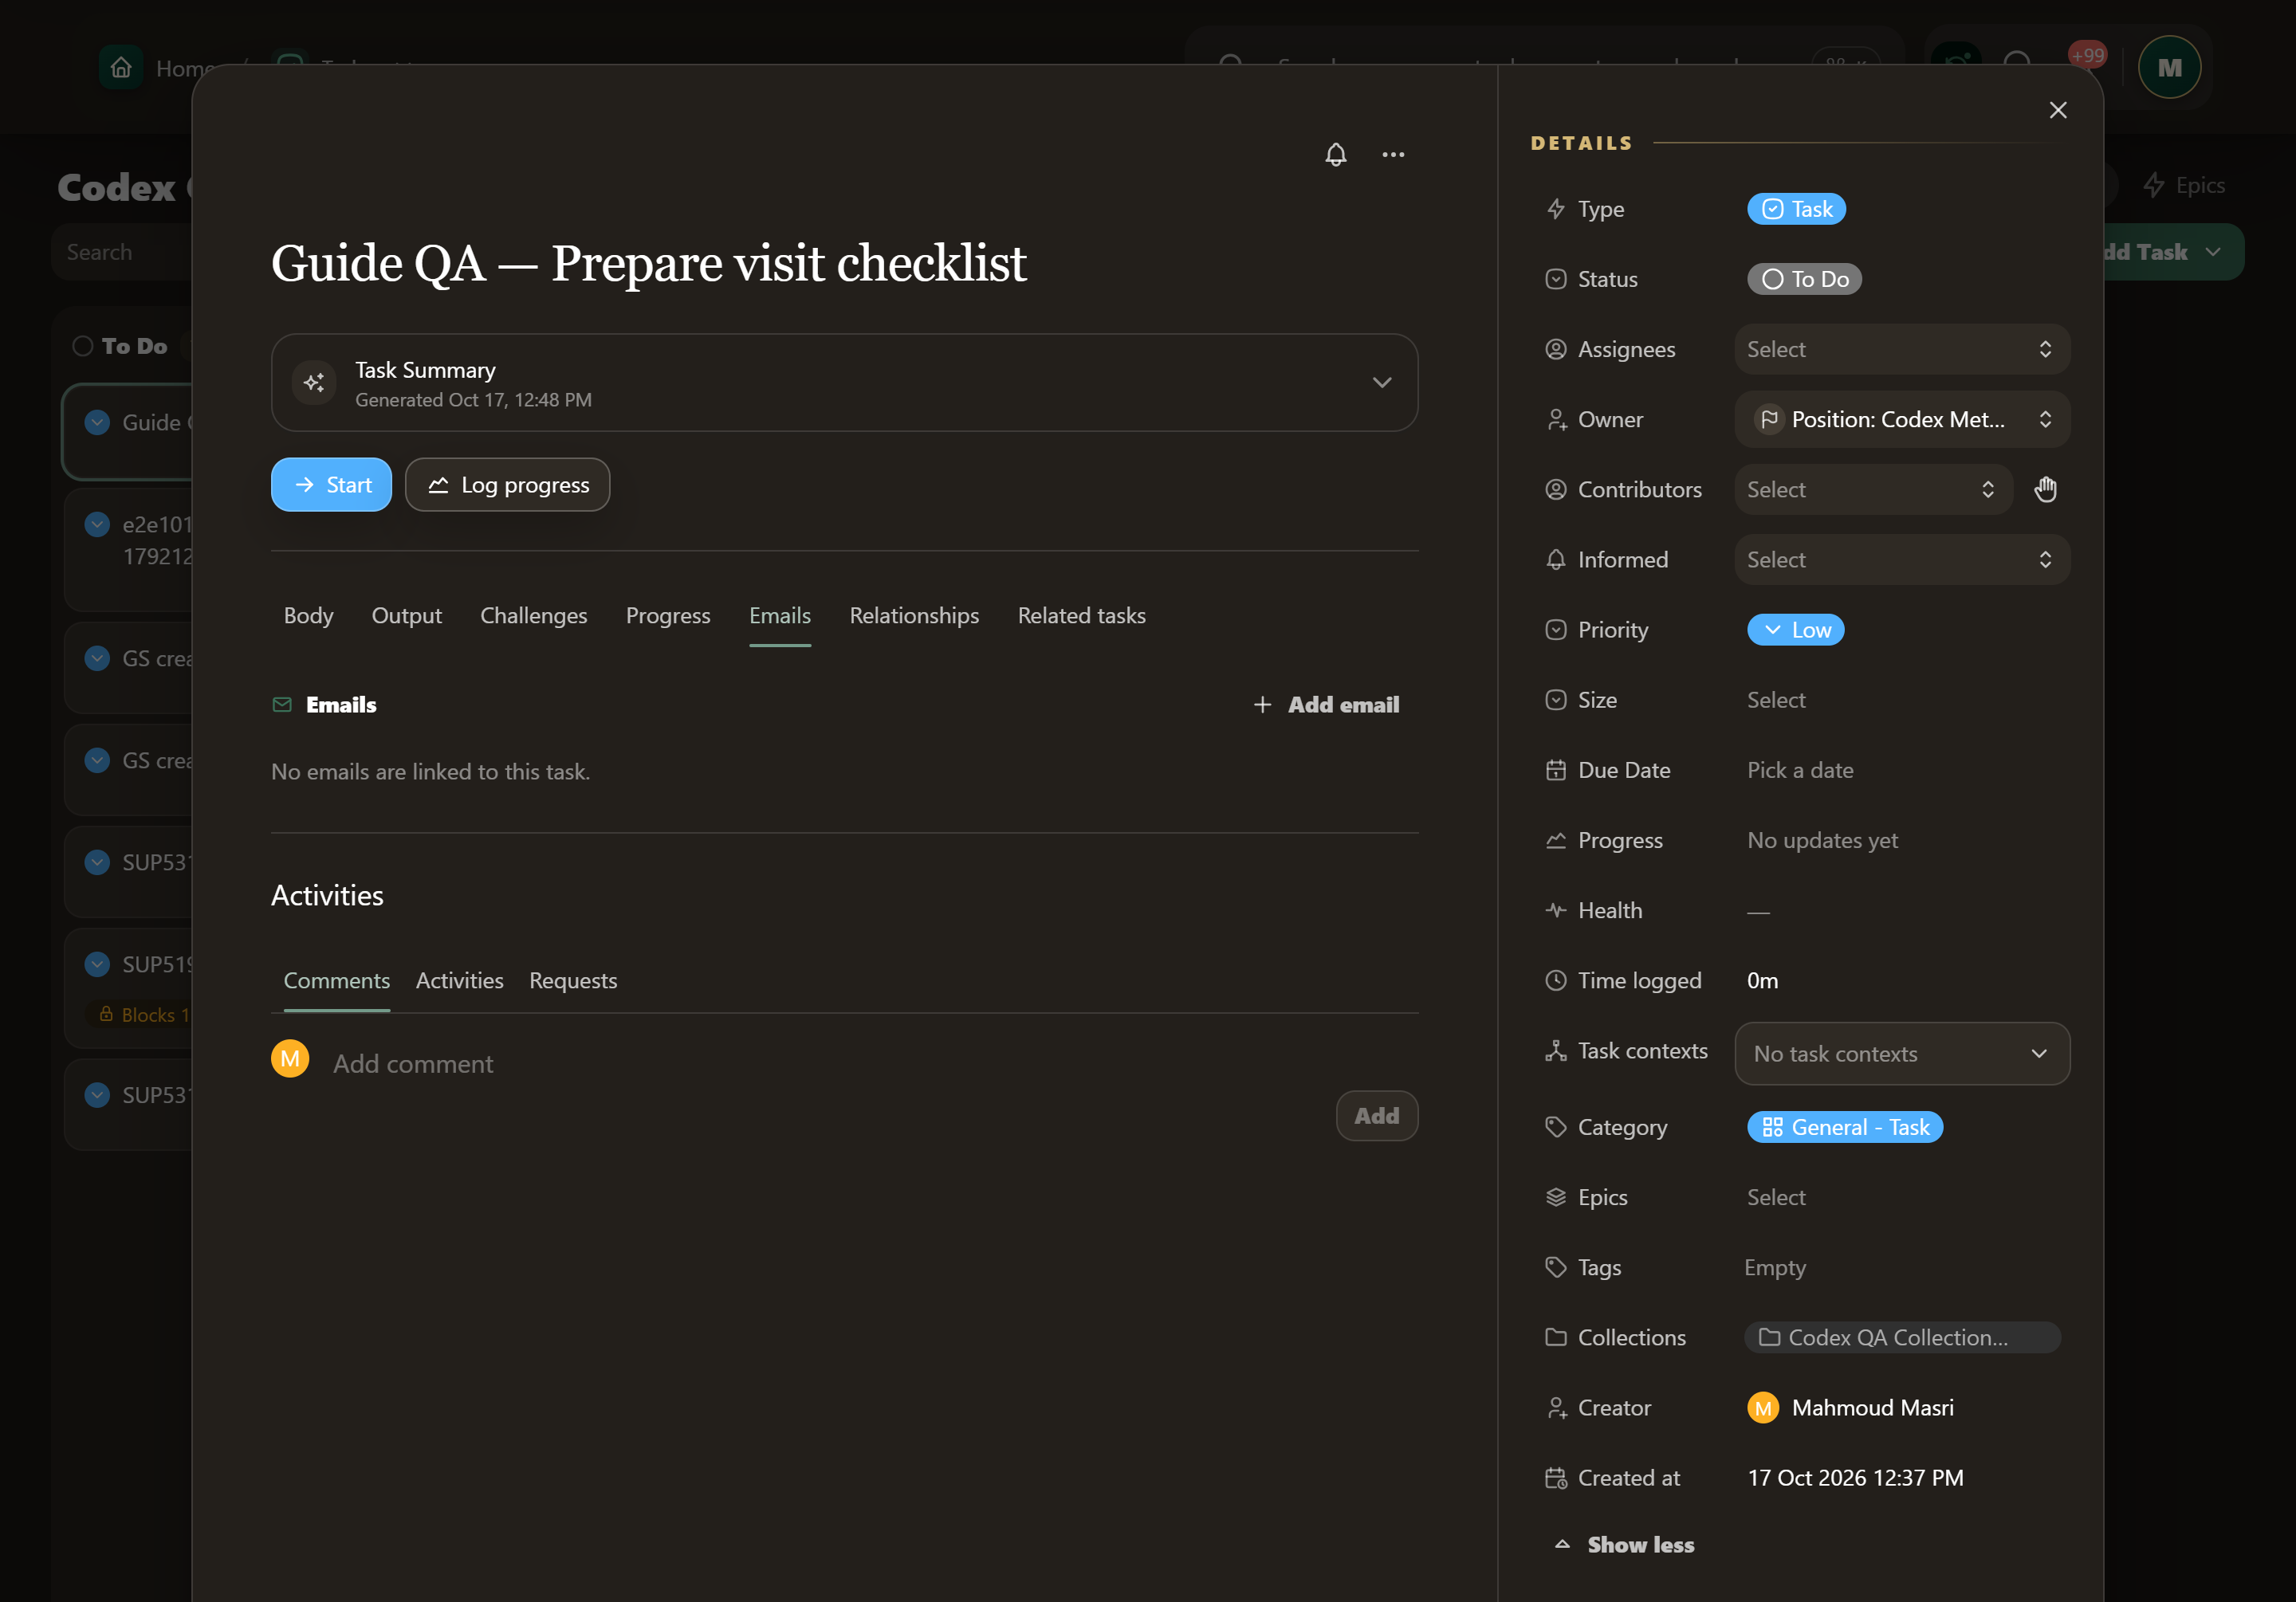
\includegraphics[width=0.95\linewidth,height=0.72\textheight,keepaspectratio]{figures/screens/ch04-emails-en.png}
\caption{Linked email}
\label{fig:tasks-relationships-emails}
\shotnote{The Emails tab collects correspondence linked to the task, and Add email links another message, so the team can find the original request without searching the mailbox. The list is empty here; do not assume a message is linked unless it appears in this tab.}
\end{figure}

\begin{table}[H]
\centering
\caption{What can you record or do?}
\label{tab:tasks-relationships-data}
\begin{tabularx}{\linewidth}{R{3.6cm} Y}
\rcHeaderRow
\thh{Section} & \thh{Content and action}\\
Relationships & Relationship meaning, entity type, record and an optional note. The task type may require links at creation or completion.\\
Related tasks & Task-to-task relations such as blockers or parent/child where enabled. Search can include other accessible collections.\\
Emails and contexts & Email supplies correspondence context; project and planning contexts connect execution to broader work when available.\\
\end{tabularx}
\end{table}

\begin{figure}[H]
\centering
\begin{tikzpicture}[node distance=0.5cm]
\node[stepBox] (a) {\RL{Choose relationship}\\\RL{meaning}};
\node[stepBox,below=of a] (b) {\RL{Select record}\\\RL{or task}};
\node[stepBox,below=of b] (c) {\RL{Verify target}\\\RL{and direction}};
\draw[flowsTo] (a) -- (b);
\draw[flowsTo] (b) -- (c);
\end{tikzpicture}
\rclegend
\caption{Steps to follow}
\label{fig:tasks-relationships-flow}
\shotnote{Correct linking starts from meaning, not from the record: decide whether the link is a source, evidence or a dependency, find the matching record or task, then verify the target and direction. A reversed relation can make the wrong task the one that waits.}
\end{figure}

\subsection{Steps and verification}
\begin{enumerate}
\item In Relationships choose Link record, select relationship and entity type, find the correct record and save.
\item In Related tasks choose Add relation, select the relationship and task, and verify direction before confirming.
\item Open the saved link and verify its target. Review blocking tasks before attempting completion.
\end{enumerate}

\textbf{Check and recovery:} If a record is absent, check type, search and permissions. Do not remove a valid dependency to bypass completion rules or treat a link as approval or an automatic record update.

\clearpage
\section{Epics}
\label{sec:tasks-feature-epics}

An epic groups tasks around a broader outcome. Use it when work needs to be split while retaining a single view of the goal.

\textbf{Where and who:} Tasks → collection → Epics tab. For the person coordinating a larger piece of work.

\begin{rcnote}[Example: Horizon]
Sarah organizes “Prepare the Aleppo branch visit” as an epic. Omar’s checklist task and a separate scheduling task belong to it.
\end{rcnote}

\begin{figure}[H]
\centering
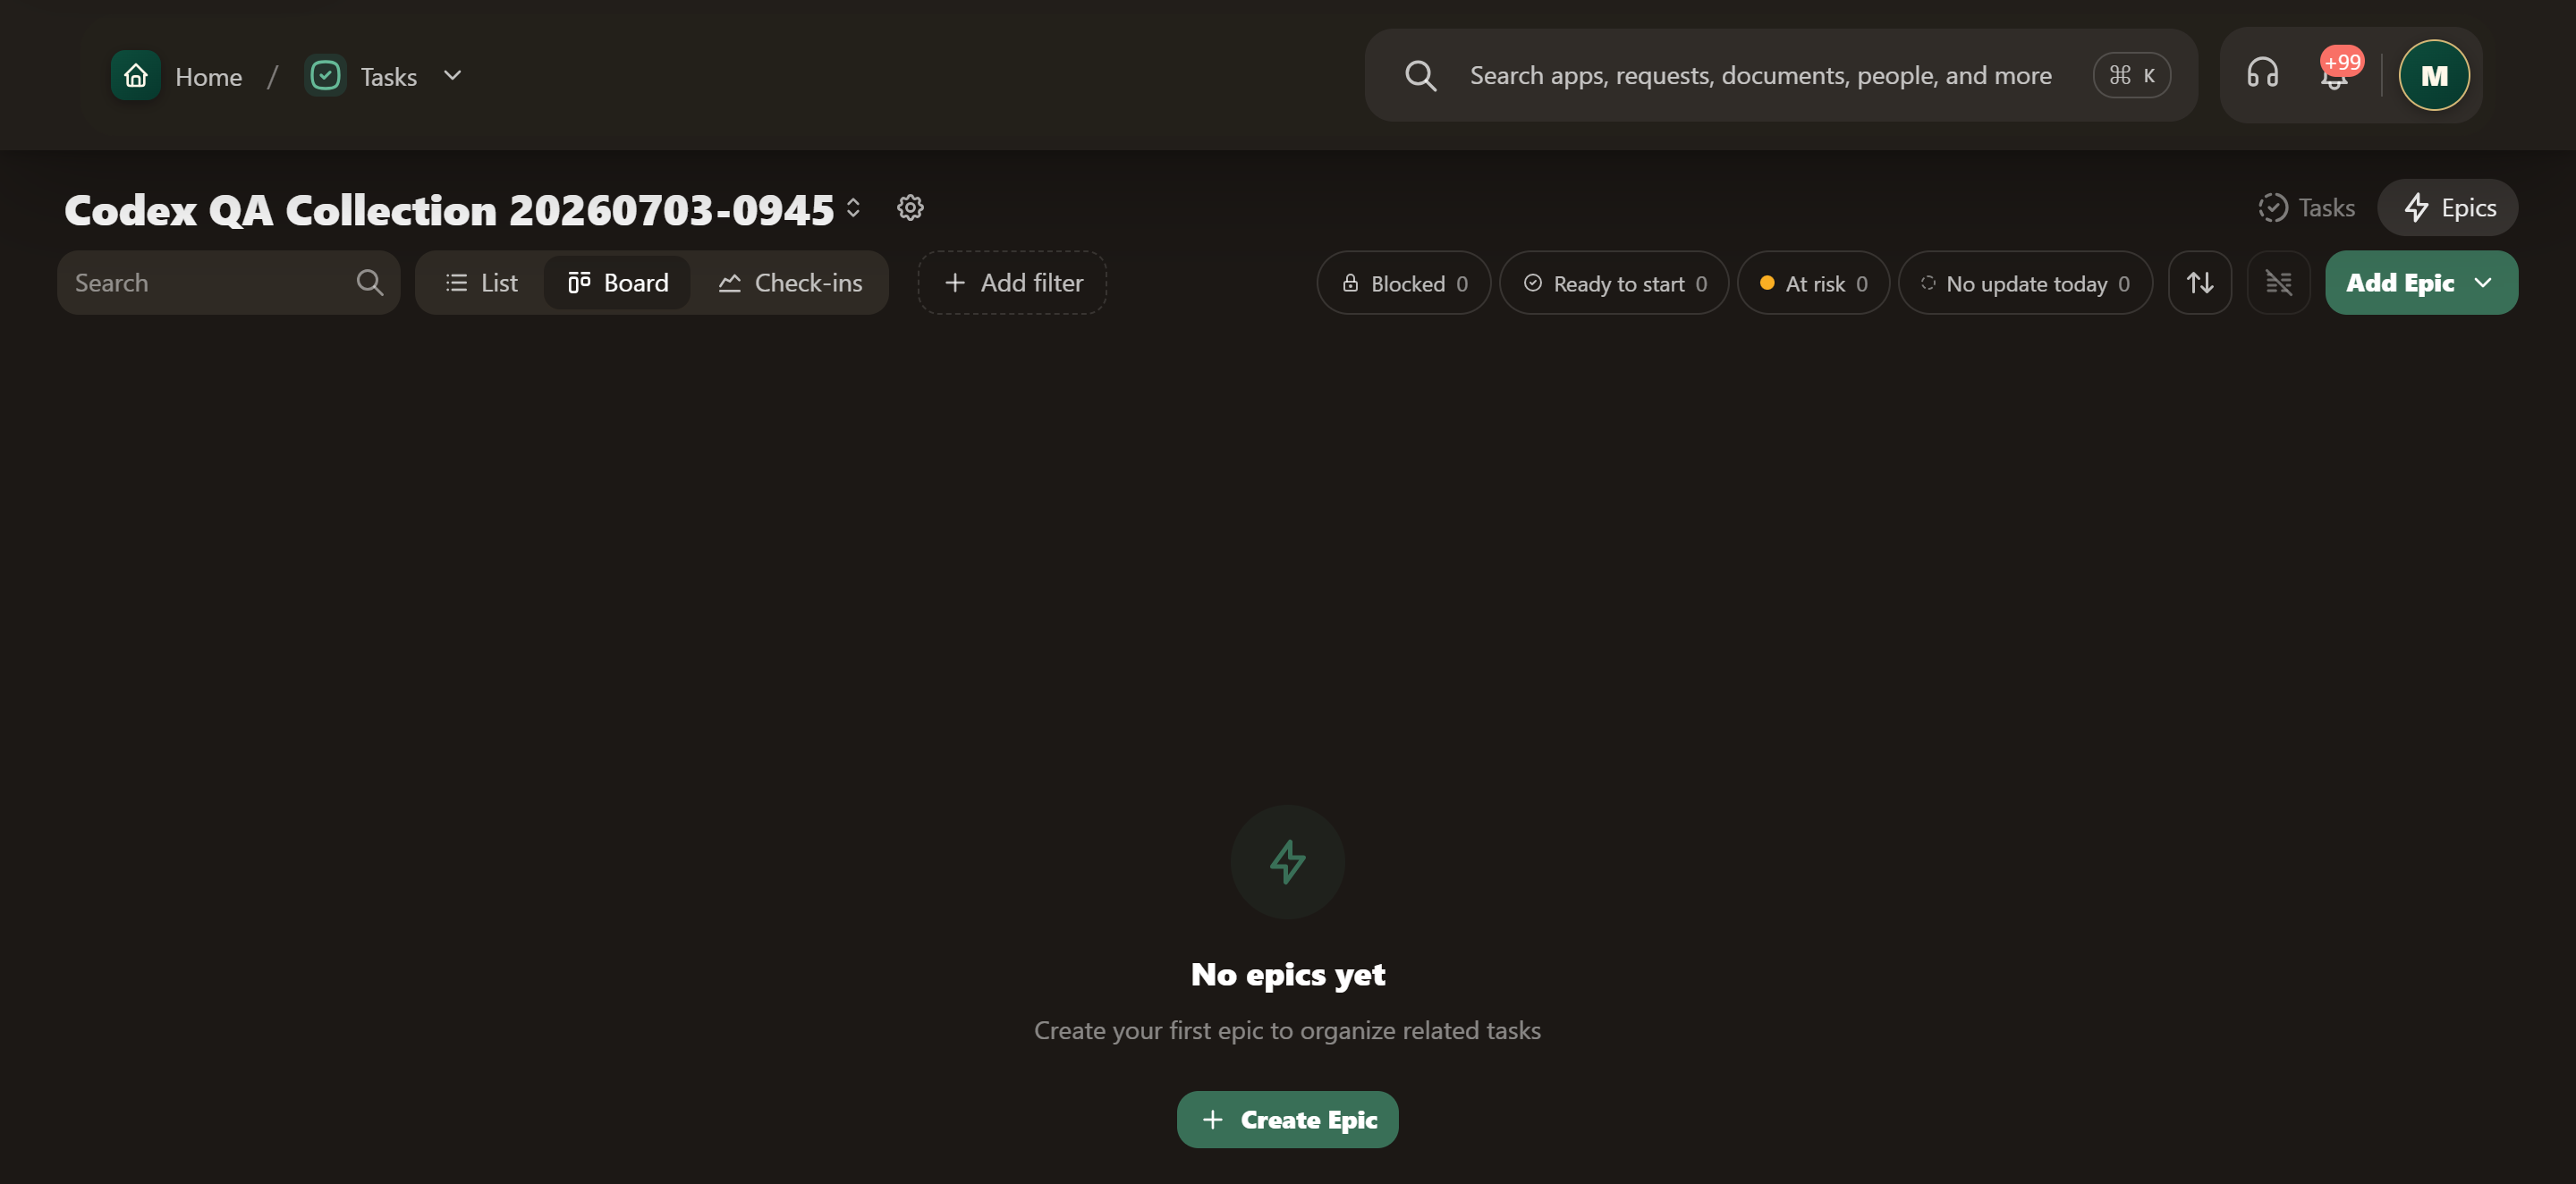
\includegraphics[width=0.95\linewidth,height=0.72\textheight,keepaspectratio]{figures/screens/ch04-epics-en.png}
\caption{Epics tab}
\label{fig:tasks-epics-epics}
\shotnote{The Epics tab inside a collection shows epics with the same view tools you use for tasks and adds an Add Epic button. It is empty in this test collection. In the Arabic interface this tab is labelled “Projects”, but it does not open the Projects and planning app.}
\end{figure}

\begin{table}[H]
\centering
\caption{What can you record or do?}
\label{tab:tasks-epics-data}
\begin{tabularx}{\linewidth}{R{3.6cm} Y}
\rcHeaderRow
\thh{Section} & \thh{Content and action}\\
Details and content & Title, type, status, responsibilities, timing and content according to the epic type.\\
Linked tasks & Create or link a task, open it or unlink it as permitted. Unlinking is different from deleting the task.\\
\end{tabularx}
\end{table}

\begin{figure}[H]
\centering
\begin{tikzpicture}[node distance=0.5cm]
\node[stepBox] (a) {\RL{Define broader}\\\RL{outcome}};
\node[stepBox,below=of a] (b) {\RL{Link tasks}};
\node[stepBox,below=of b] (c) {\RL{Review each result}};
\draw[flowsTo] (a) -- (b);
\draw[flowsTo] (b) -- (c);
\end{tikzpicture}
\rclegend
\caption{Steps to follow}
\label{fig:tasks-epics-flow}
\shotnote{The diagram shows that an epic is a tracking frame, not a replacement for tasks: define the broader outcome, link the tasks that achieve it, and follow each task’s result separately. You then assess the whole piece of work from its parts, not from the epic’s status alone.}
\end{figure}

\subsection{Steps and verification}
\begin{enumerate}
\item Open Epics, choose Add Epic and an available type. Enter the broader outcome and responsibility, then create.
\item Inside the epic, add a task or link an existing one; select the correct work item and confirm.
\item Open the linked task and verify the relationship. Review each task before updating the epic.
\end{enumerate}

\textbf{Check and recovery:} Do not assume closing an epic also closes its tasks or a linked project; review their outcomes and statuses separately.

\clearpage
\section{AI suggestions}
\label{sec:tasks-feature-suggestions}

A suggestion is proposed work derived from email context, awaiting review before becoming an active task. Check its source, responsibility and timing before accepting.

\textbf{Where and who:} Tasks → AI suggestions card, when enabled. For an authorized reviewer.

\begin{rcnote}[Example: Horizon]
Sarah reviews a suggestion to confirm a Horizon visit, selects Horizon visits at acceptance, then corrects the date on the resulting task.
\end{rcnote}

\begin{figure}[H]
\centering
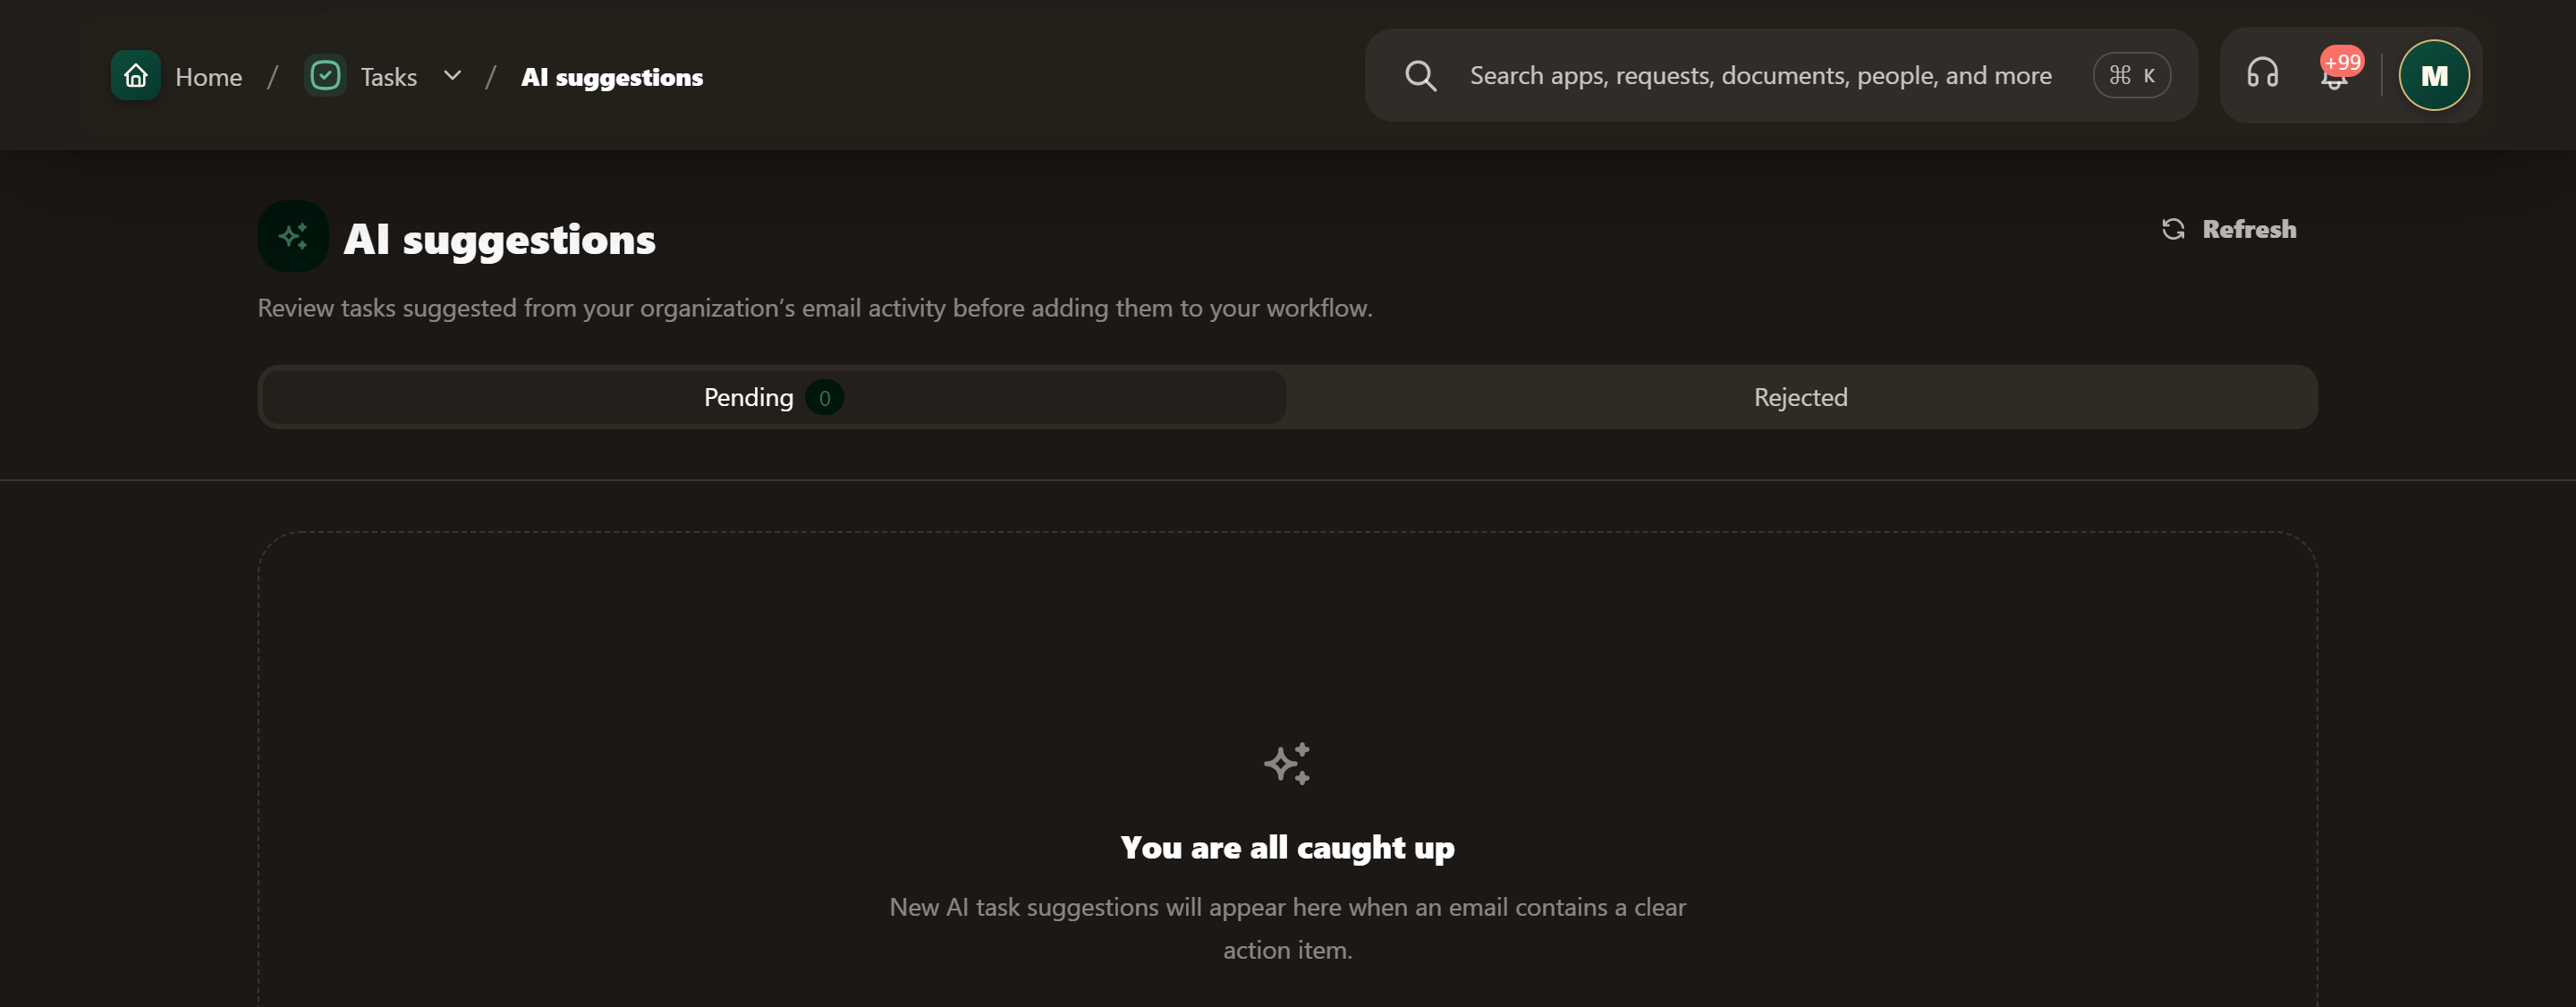
\includegraphics[width=0.95\linewidth,height=0.72\textheight,keepaspectratio]{figures/screens/ch04-suggestions-en.png}
\caption{Suggestion queue}
\label{fig:tasks-suggestions-suggestions}
\shotnote{This page holds tasks suggested from email in two tabs: Pending for items awaiting your decision and Rejected for those you dismissed, so a suggestion enters the workflow only after a reviewer accepts it. The queue was empty in test2 at capture time, so acceptance was not tested here.}
\end{figure}

\begin{table}[H]
\centering
\caption{What can you record or do?}
\label{tab:tasks-suggestions-data}
\begin{tabularx}{\linewidth}{R{3.6cm} Y}
\rcHeaderRow
\thh{Section} & \thh{Content and action}\\
Status and source & Filter suggestions, open details and review the email source.\\
Accept or reject & Acceptance needs an allowed collection and type and valid details; rejection does not complete a task.\\
\end{tabularx}
\end{table}

\begin{figure}[H]
\centering
\begin{tikzpicture}[node distance=0.5cm]
\node[stepBox] (a) {\RL{Read source}};
\node[stepBox,below=of a] (b) {\RL{Review suggestion}};
\node[stepBox,below=of b] (c) {\RL{Accept and verify}};
\draw[flowsTo] (a) -- (b);
\draw[flowsTo] (b) -- (c);
\end{tikzpicture}
\rclegend
\caption{Steps to follow}
\label{fig:tasks-suggestions-flow}
\shotnote{The diagram puts reading the source before any decision, because the email explains why the suggestion exists and who asked. Reviewing its details follows, then acceptance and checking the resulting task; a suggestion becomes a task only by a reviewer’s decision.}
\end{figure}

\subsection{Steps and verification}
\begin{enumerate}
\item Open AI suggestions and choose Pending. If a suggestion exists, open it and read its source.
\item Review the suggestion and its source. Select a task type and at least one collection, then confirm acceptance; or reject unsuitable work.
\item After acceptance open the resulting task, correct title, people and date as needed, and verify saving. With an empty queue there is no acceptance action to perform.
\end{enumerate}

\textbf{Check and recovery:} If a required type is missing, check creation permission and collection restrictions. A suggestion alone is not a confirmed assignment.

\clearpage
\section{Assignments}
\label{sec:tasks-feature-assignments}

Assignments show forms you have been asked to fill and their related work. Start from the assignment and return to its outcome; form design and assignment-plan administration use other tools.

\textbf{Where and who:} Tasks → Assignments. For the person asked to fill a form.

\begin{rcnote}[Example: Horizon]
Omar opens the assigned Horizon visit form, completes it and submits it. Sarah reviews its outcome through the form workflow.
\end{rcnote}

\begin{figure}[H]
\centering

\includegraphics[width=0.95\linewidth,height=0.72\textheight,keepaspectratio]{figures/screens/ch04-assignments-en.png}
\caption{Assignments list}
\label{fig:tasks-assignments-assignments}
\shotnote{The page gathers the work requested from you under Assigned to me, grouped by due date, and each assignment offers a button suited to its state to start or continue filling it. Switching between Open and Finished shows current or earlier work, while the Plans tab is for monitoring distribution. A Today’s work card appears when an assignment can be downloaded for offline work.}
\end{figure}

\begin{table}[H]
\centering
\caption{What can you record or do?}
\label{tab:tasks-assignments-data}
\begin{tabularx}{\linewidth}{R{3.6cm} Y}
\rcHeaderRow
\thh{Section} & \thh{Content and action}\\
Assignment card & Form title, due date, status and available outcome.\\
Actions & Start, continue or view; claim or decline where allowed; an outcome without an answer may require a reason, photo or location before closure.\\
Assigned to me and Plans & Assigned to me groups your assignments by urgency. Plans opens distribution monitoring for authorized users.\\
Packages and field work & A package groups related forms and shows the next module. Offline download and Outbox appear for eligible work; verify synchronization when back online.\\
Availability and ordering & Away until records unavailability. Group ordering or a map may be available depending on the work data.\\
\end{tabularx}
\end{table}

\begin{figure}[H]
\centering
\begin{tikzpicture}[node distance=0.5cm]
\node[stepBox] (a) {\RL{Open assignment}};
\node[stepBox,below=of a] (b) {\RL{Fill and submit}};
\node[stepBox,below=of b] (c) {\RL{Review outcome}};
\draw[flowsTo] (a) -- (b);
\draw[flowsTo] (b) -- (c);
\end{tikzpicture}
\rclegend
\caption{Steps to follow}
\label{fig:tasks-assignments-flow}
\shotnote{The diagram connects the start of the work to its end: open the assignment itself to reach the correct form, fill and submit it, then review its outcome. A draft does not mean the assignment is done; what counts is submission and the outcome that follows.}
\end{figure}

\subsection{Steps and verification}
\begin{enumerate}
\item Open Assignments and select the intended work. If it is claimable, claim it before starting.
\item Choose Start or Continue, complete the form and use its submission action.
\item Return to Assignments, show Finished if needed, and choose View to verify. “Outcome without an answer” is a separate permitted action that closes work, not a read-only results button.
\end{enumerate}

\textbf{Check and recovery:} Saving a draft is different from submitting. If an assignment is missing, check recipient, plan and access with the owner.

\clearpage
\section{Task settings}
\label{sec:tasks-feature-settings}

Task settings define work types, categories and available relationships. This is administrator setup; employees normally use the existing types.

\textbf{Where and who:} Builder → Task settings. For an authorized administrator.

\begin{rcnote}[Example: Horizon]
Sarah reviews the visit-task type with the administrator: default category, status workflow and whether progress updates are required. She then uses it for Horizon tasks.
\end{rcnote}

\begin{figure}[H]
\centering
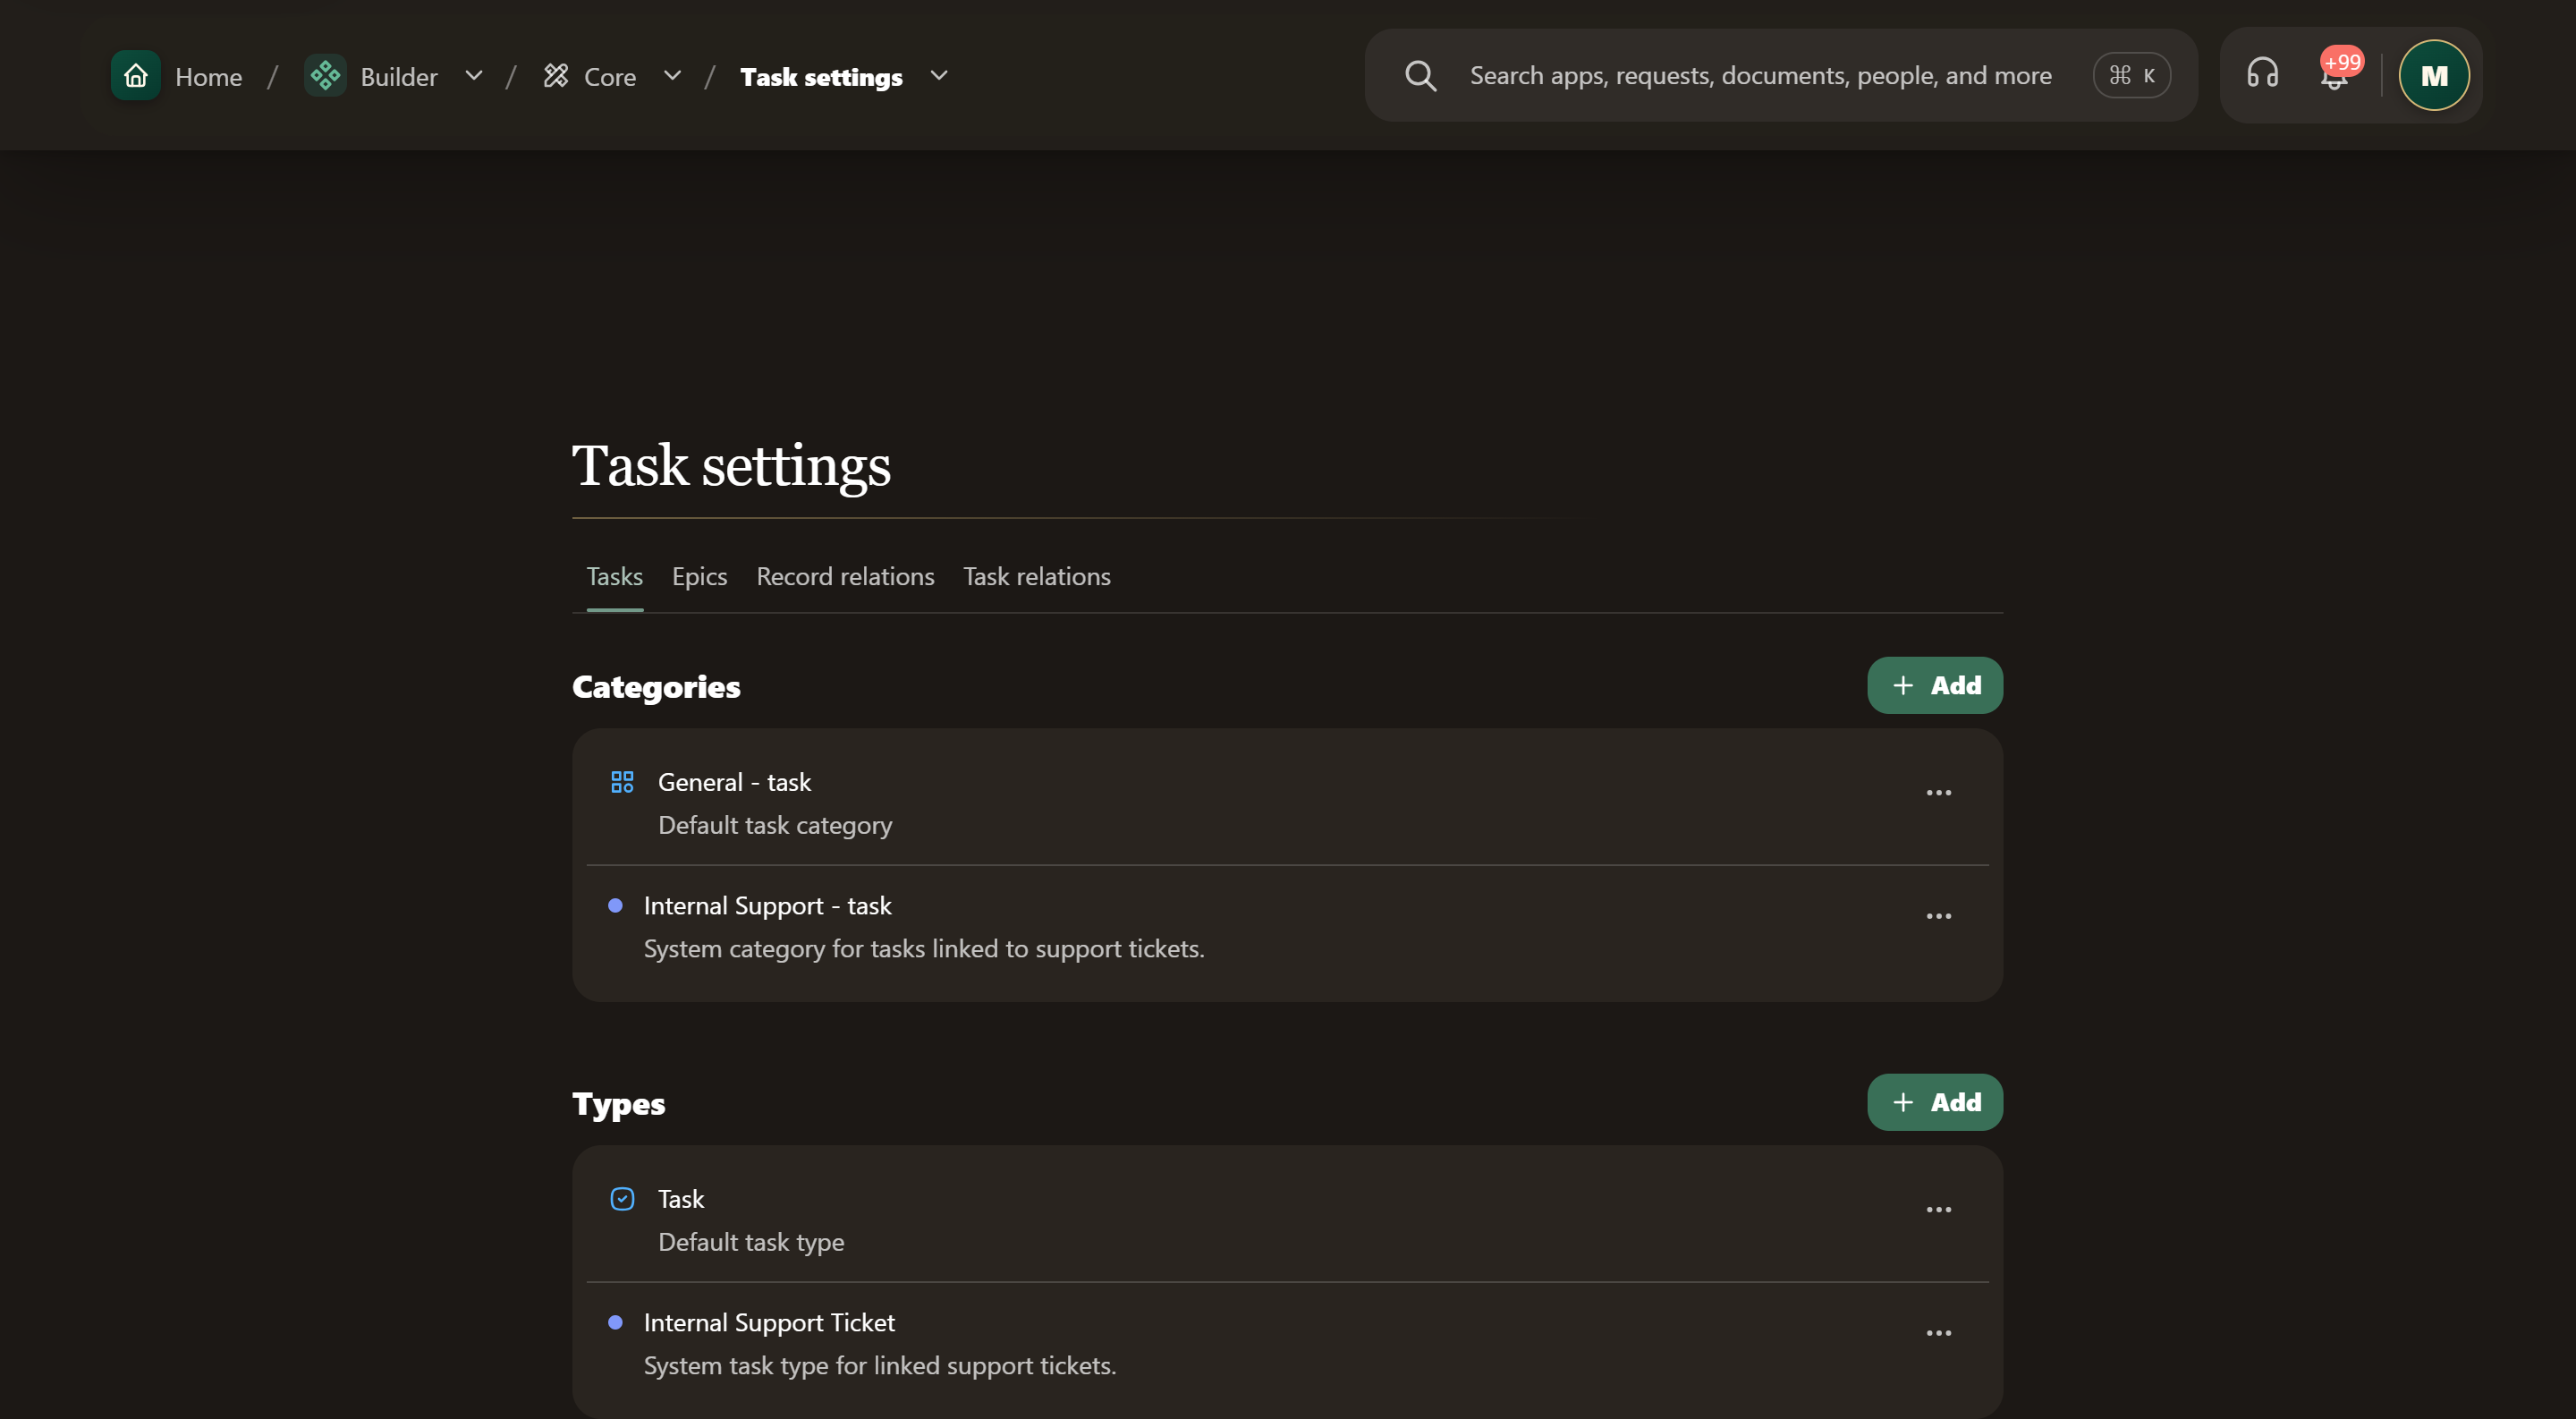
\includegraphics[width=0.95\linewidth,height=0.72\textheight,keepaspectratio]{figures/screens/ch04-settings-en.png}
\caption{Task type settings}
\label{fig:tasks-settings-settings}
\shotnote{Task settings splits configuration into four tabs: Tasks, Epics, Record relations and Task relations. The Tasks tab lists the categories and types users choose from when creating a task, including the default category and type. Because a change here affects every task using the type, review its impact before changing it.}
\end{figure}

\begin{figure}[H]
\centering
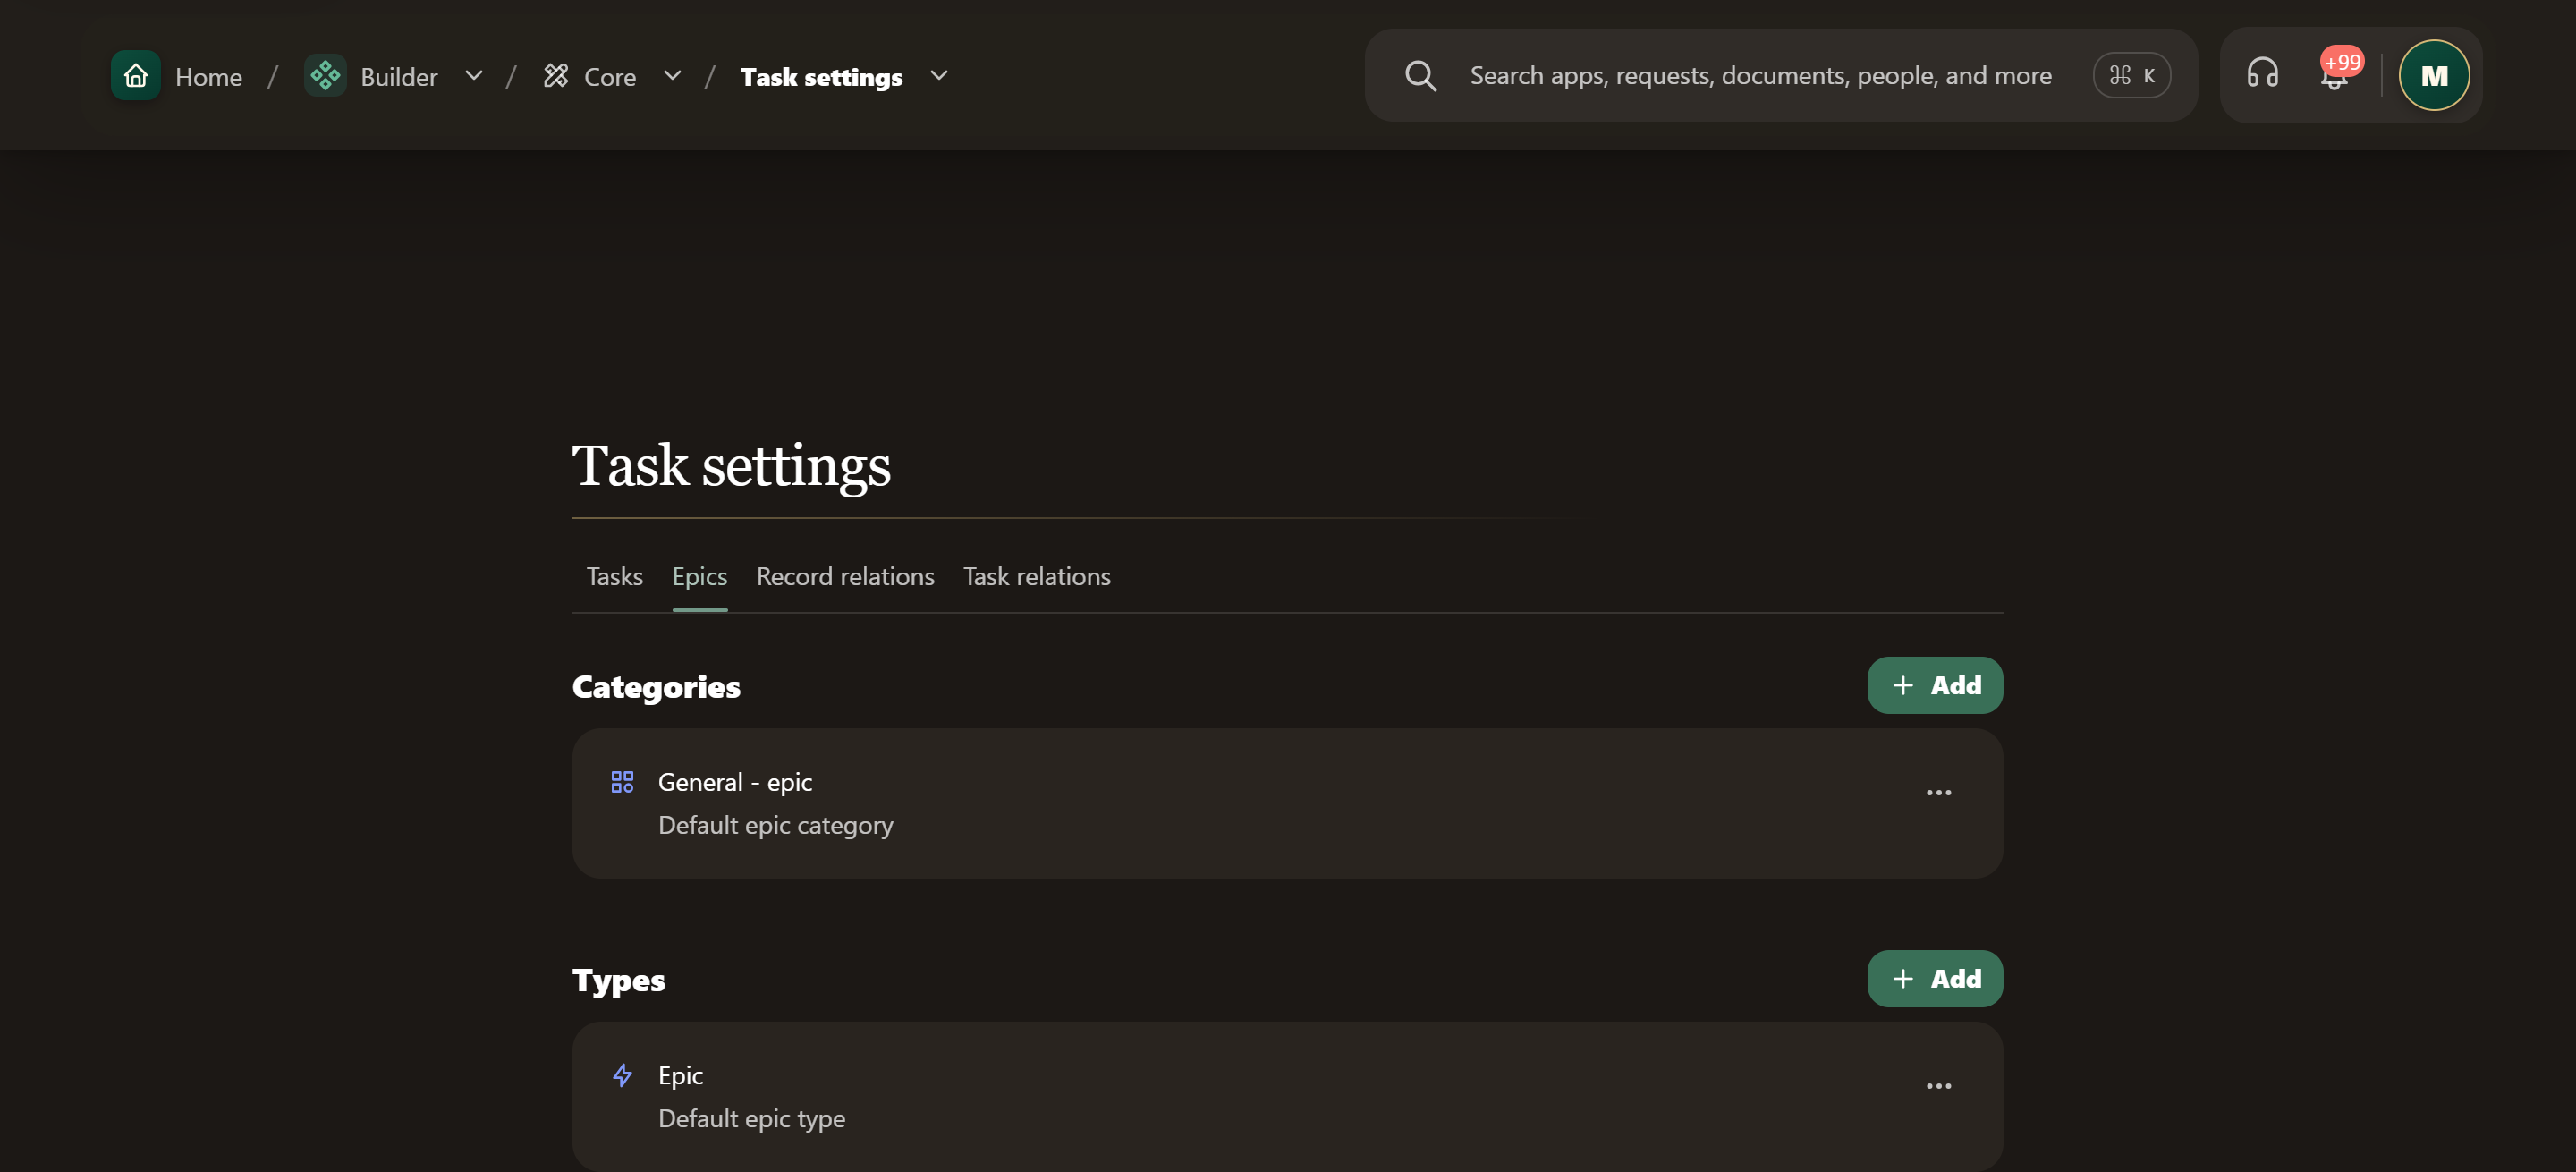
\includegraphics[width=0.95\linewidth,height=0.72\textheight,keepaspectratio]{figures/screens/ch04-settings-epics-en.png}
\caption{Epic settings}
\label{fig:tasks-settings-settings-epics}
\shotnote{The Epics tab here configures epic categories and types separately from ordinary task categories; test2 shows the default epic type. It has no connection to the Projects and planning app despite the similar Arabic name.}
\end{figure}

\begin{figure}[H]
\centering
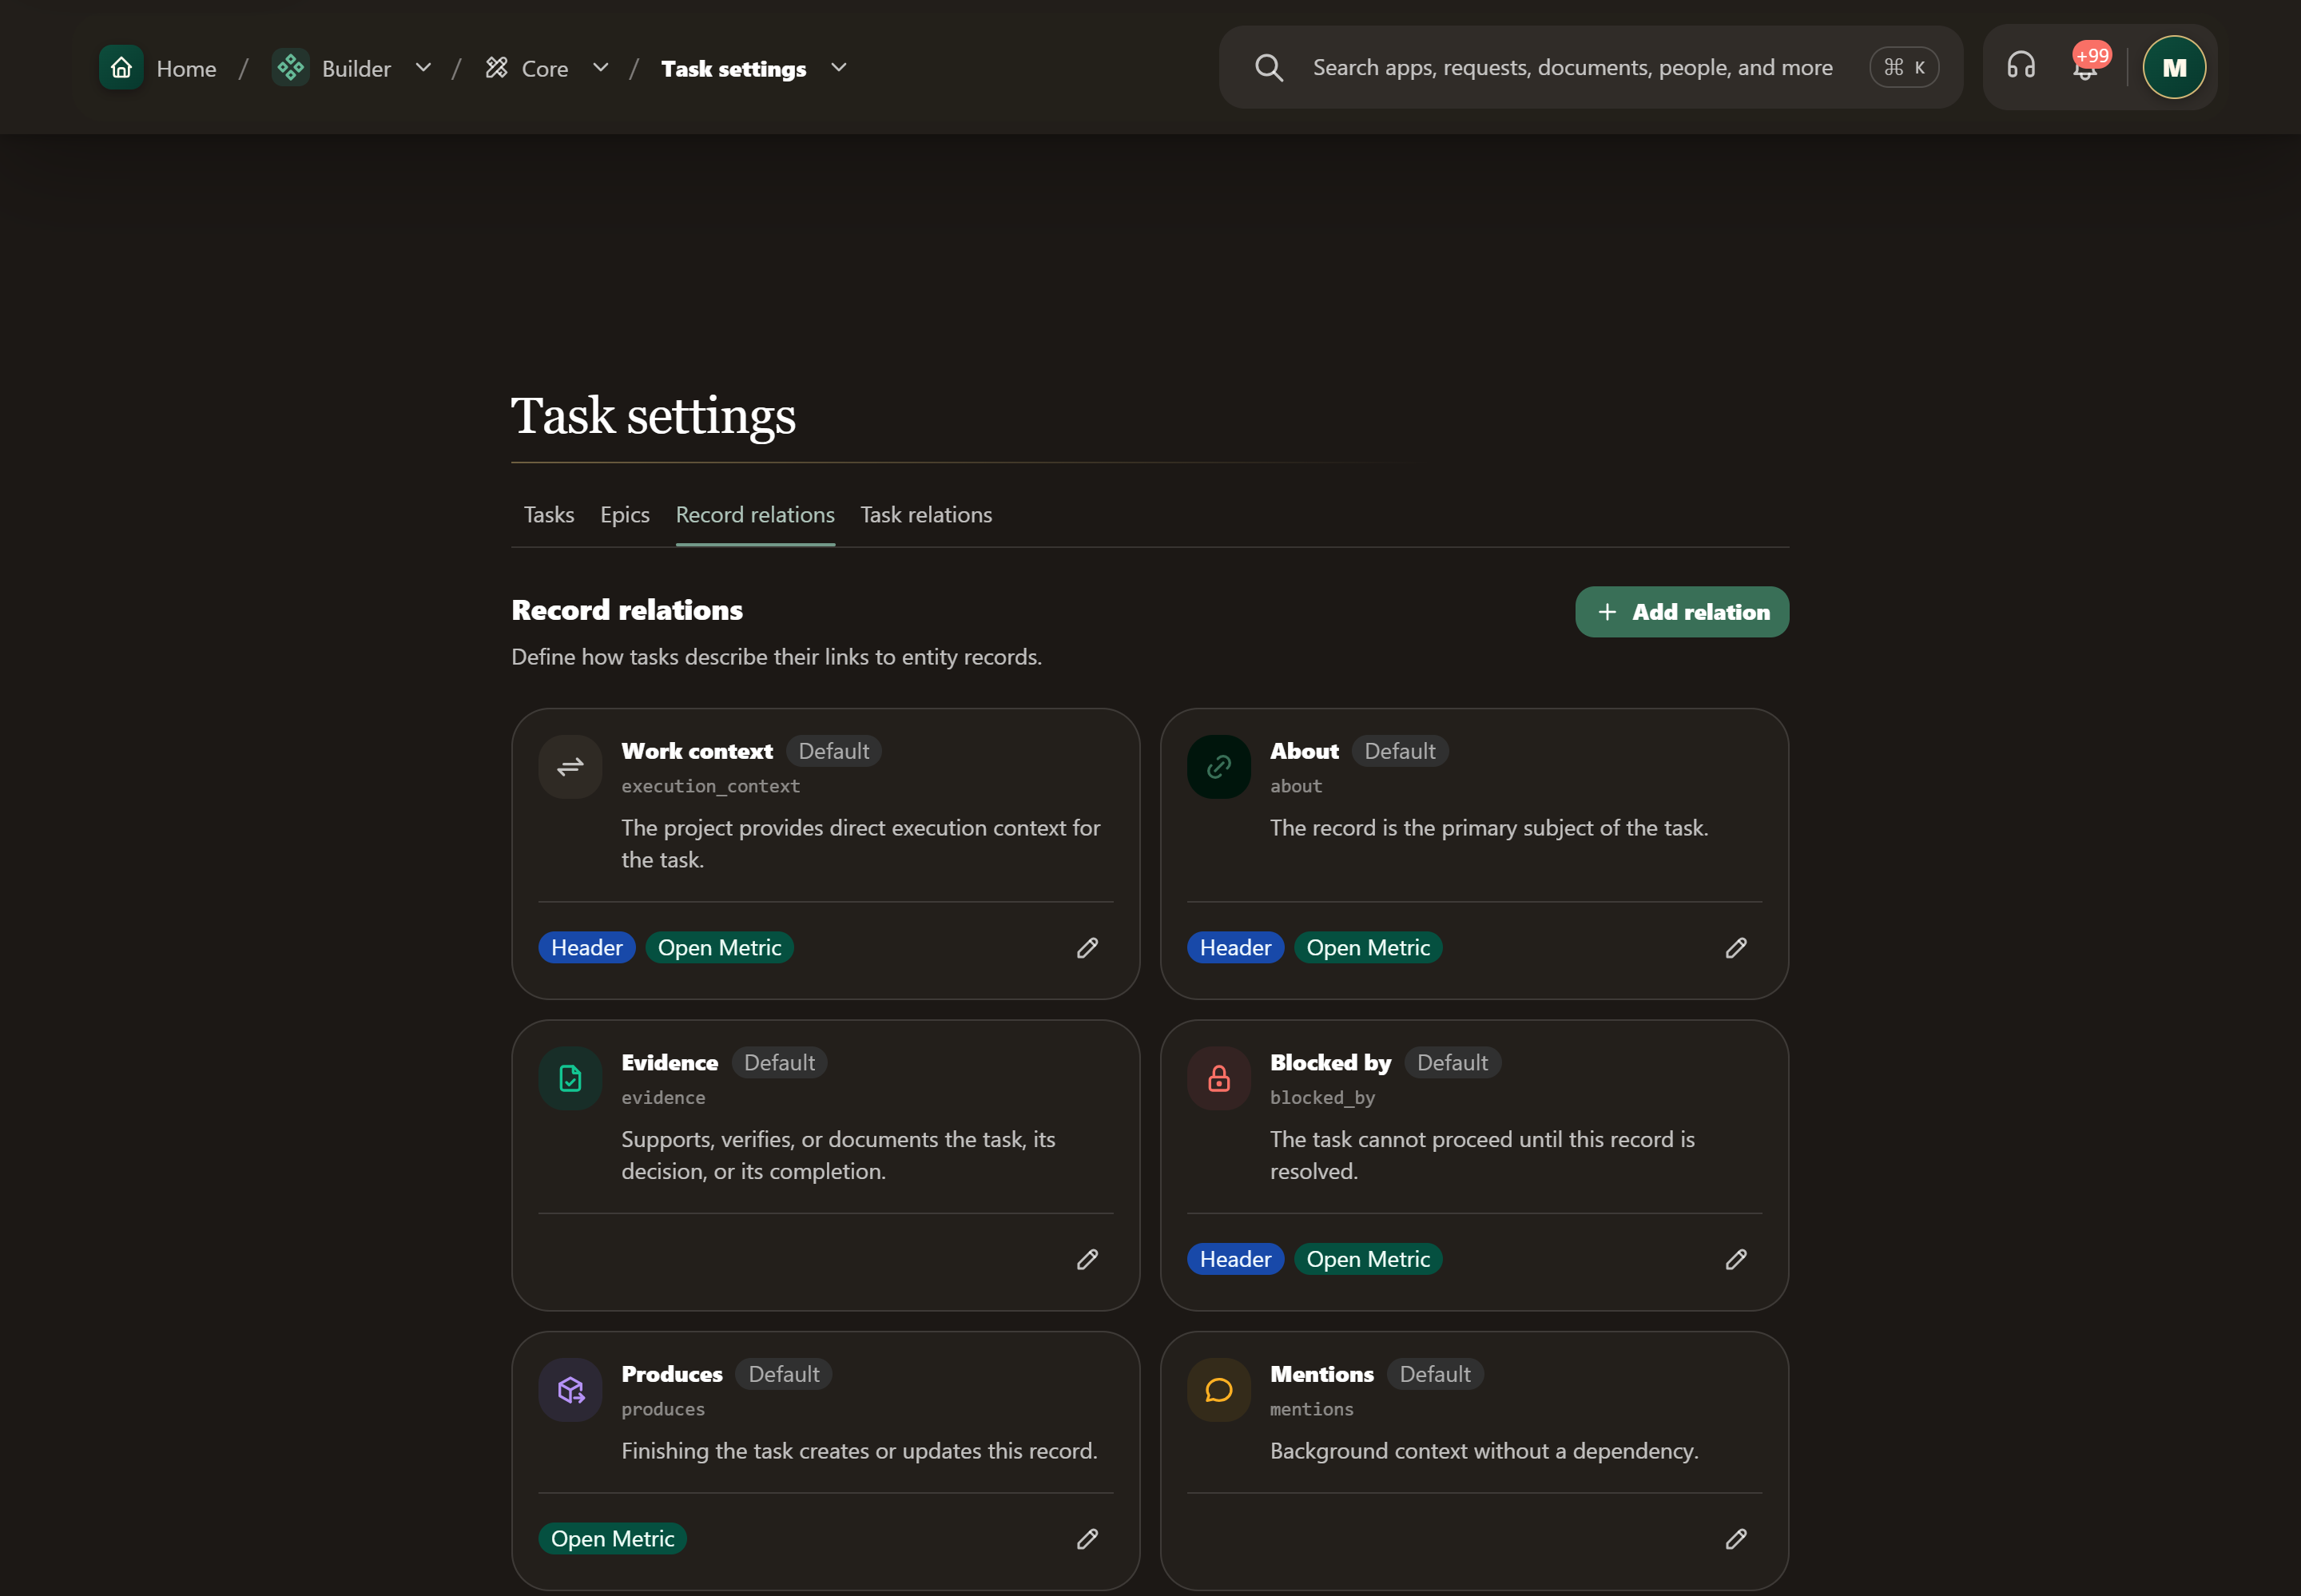
\includegraphics[width=0.95\linewidth,height=0.72\textheight,keepaspectratio]{figures/screens/ch04-settings-records-en.png}
\caption{Record relationship settings}
\label{fig:tasks-settings-settings-records}
\shotnote{The Record relations tab defines the meanings you choose from when linking a task to a record, such as Evidence, Produces and Blocked by, each with a description of its effect. Colleagues then understand why a link exists, not merely that it does. The defaults appear here; an administrator adds others with Add relation.}
\end{figure}

\begin{figure}[H]
\centering
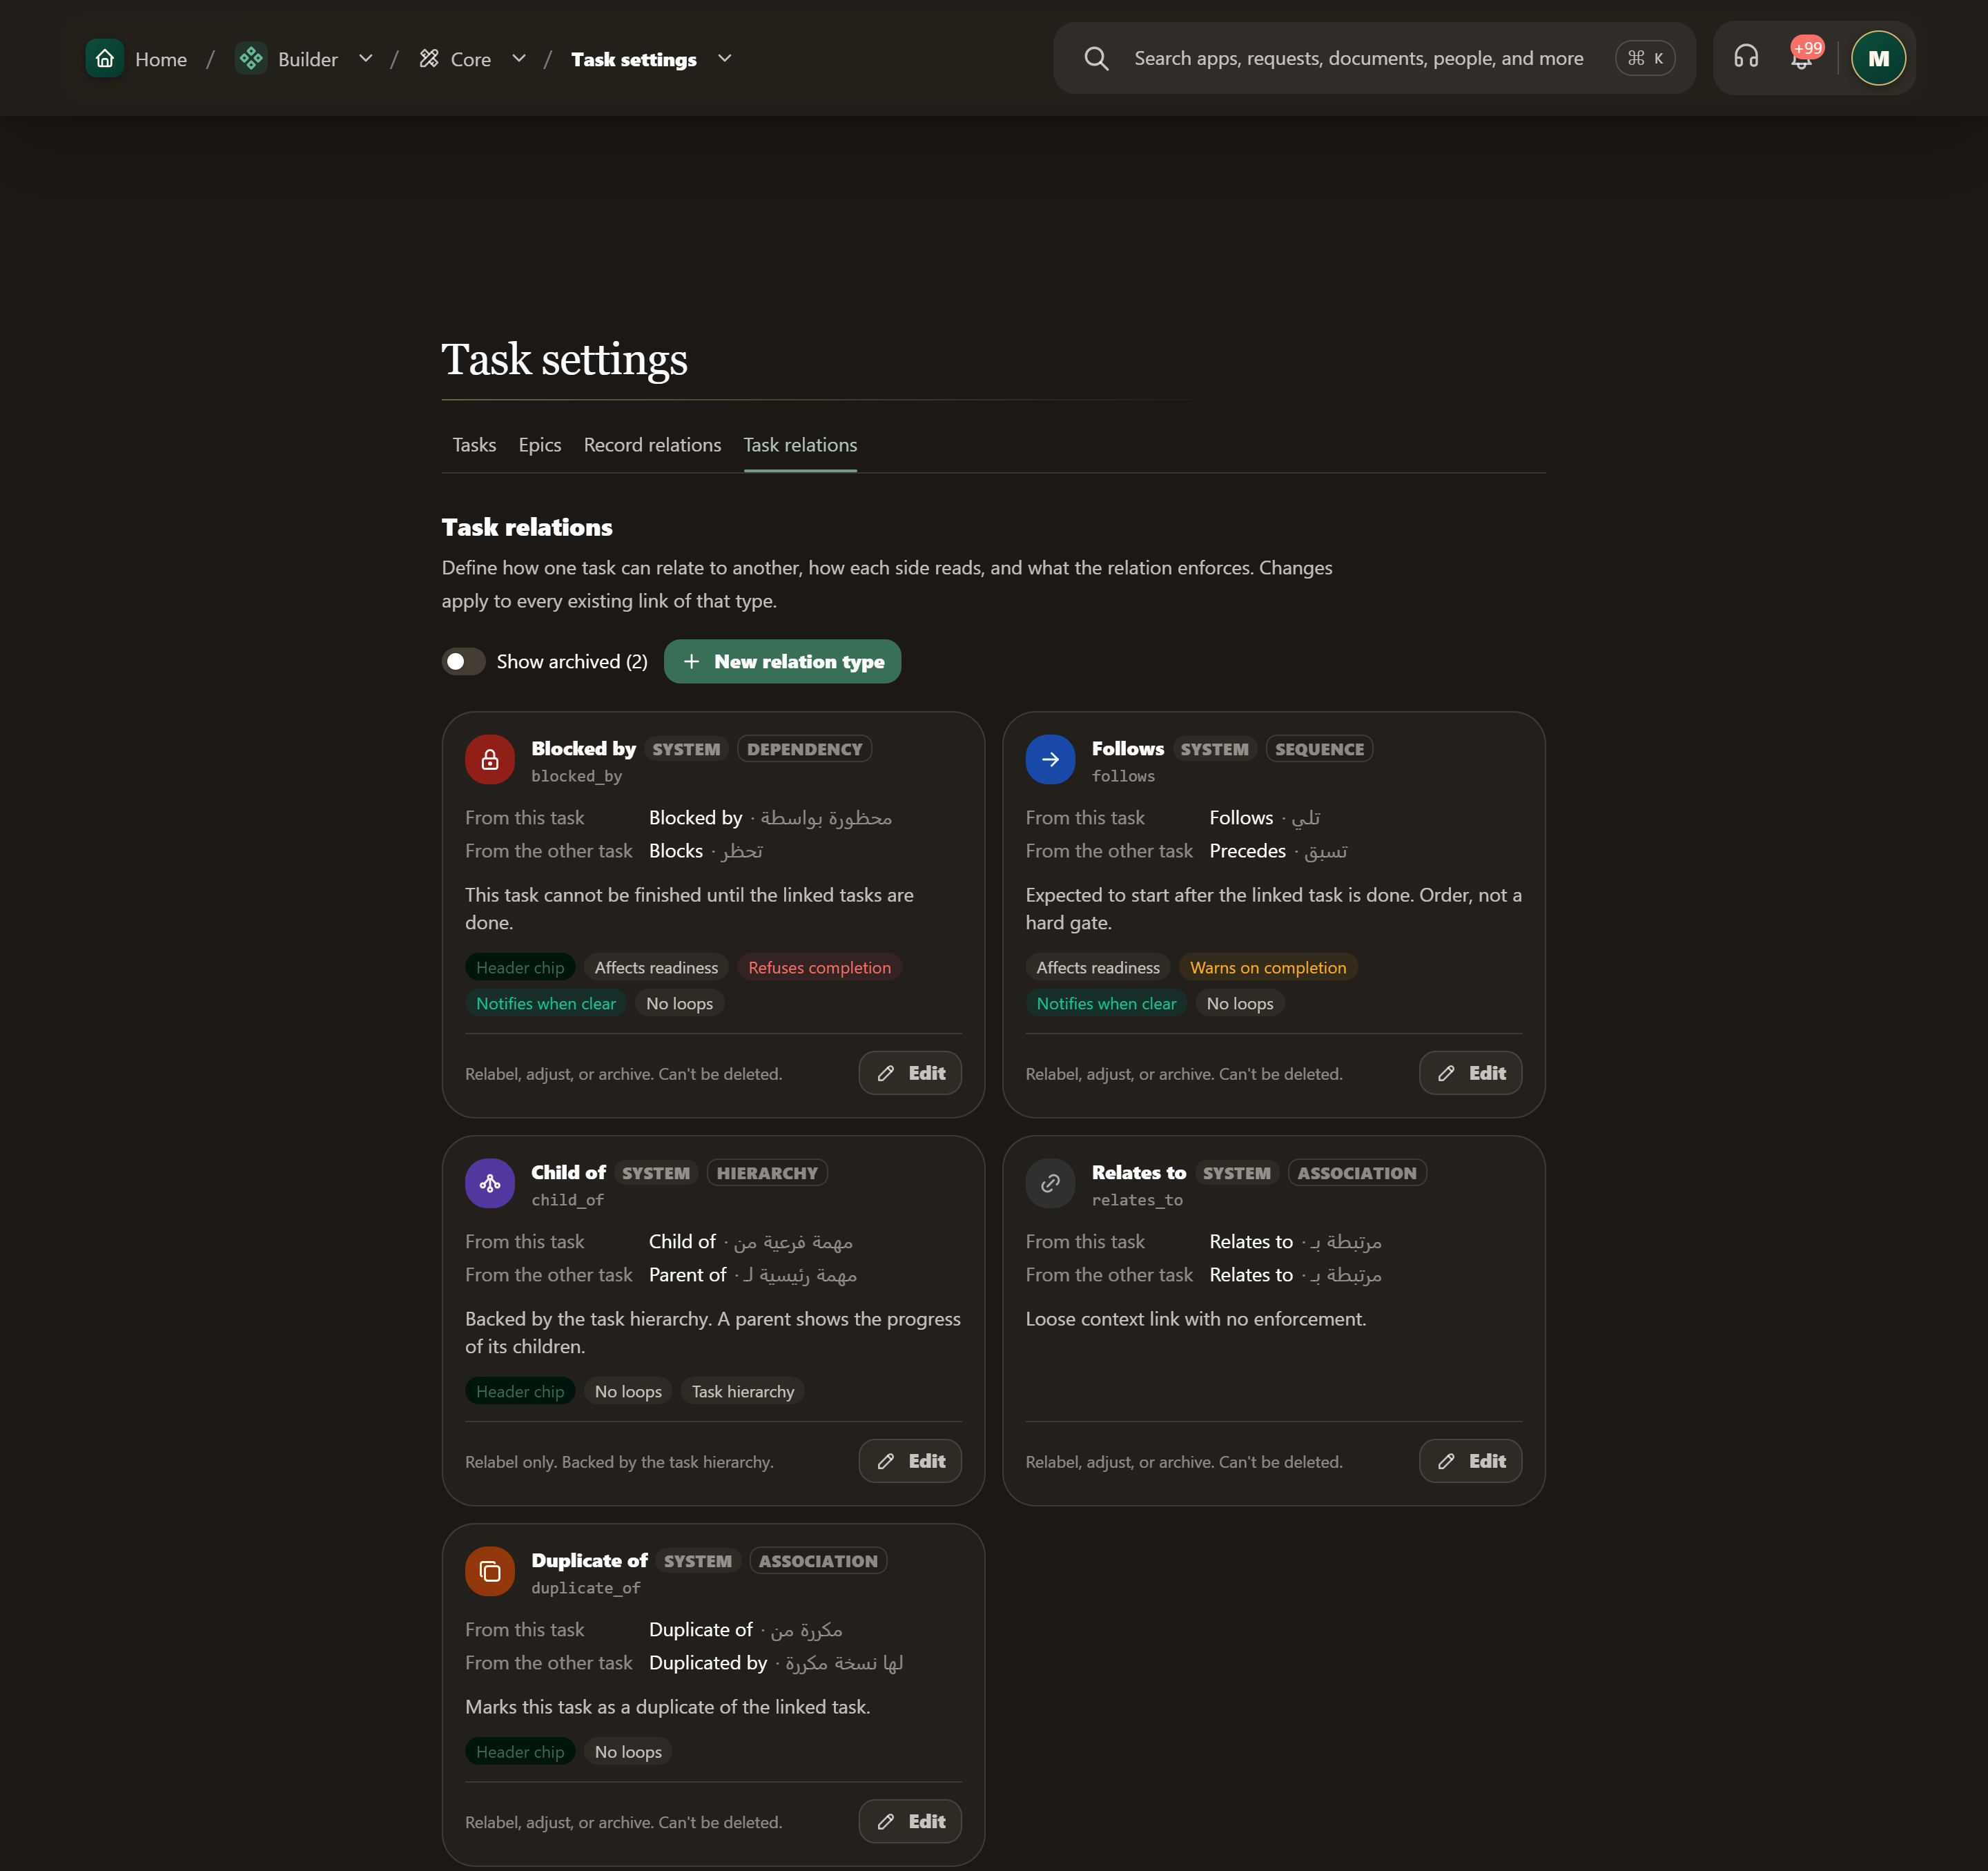
\includegraphics[width=0.95\linewidth,height=0.72\textheight,keepaspectratio]{figures/screens/ch04-settings-relations-en.png}
\caption{Task relationship settings}
\label{fig:tasks-settings-settings-relations}
\shotnote{The Task relations tab defines how one task relates to another and how each side reads the relation, such as Blocked by and Child of. Their effects differ: here only the blocking relation carries Refuses completion, while others express order or association. System relations can be renamed or archived but not deleted.}
\end{figure}

\begin{table}[H]
\centering
\caption{What can you record or do?}
\label{tab:tasks-settings-data}
\begin{tabularx}{\linewidth}{R{3.6cm} Y}
\rcHeaderRow
\thh{Section} & \thh{Content and action}\\
Tasks and epics & Separate categories and types; name, description, color and icon. A type selects default category, status template and permitted participants.\\
Type rules & Required relationships and limits, plus progress-update configuration and cadence where available.\\
Record and task relationships & Relationship types, labels, direction and restrictions. Distinguish an ordinary link from a completion blocker.\\
\end{tabularx}
\end{table}

\begin{figure}[H]
\centering
\begin{tikzpicture}[node distance=0.5cm]
\node[stepBox] (a) {\RL{Review type}};
\node[stepBox,below=of a] (b) {\RL{Set rules}};
\node[stepBox,below=of b] (c) {\RL{Test a task}};
\draw[flowsTo] (a) -- (b);
\draw[flowsTo] (b) -- (c);
\end{tikzpicture}
\rclegend
\caption{Steps to follow}
\label{fig:tasks-settings-flow}
\shotnote{The diagram starts from the type because rules belong to it: review the type, set its rules, then create a test task of that type. The test task reveals the effect on fields and transitions before it reaches the team’s daily work.}
\end{figure}

\subsection{Steps and verification}
\begin{enumerate}
\item Open Task settings and choose Tasks or Epics. Review existing categories and types before adding.
\item Open a type and review name, category, status template and permitted use. Review relationship and progress rules, then save approved changes.
\item Create a test task of that type in an appropriate collection and verify expected fields, rules and status transitions.
\end{enumerate}

\textbf{Check and recovery:} If a type is missing from creation, check collection restrictions, allowed use and permissions. Do not change shared settings merely to bypass one task error.

\clearpage
\section{Status templates}
\label{sec:tasks-feature-statuses}

A status template defines work stages and transitions. Link it to a task type so tasks use an appropriate workflow.

\textbf{Where and who:} Builder → Status templates. For the workflow administrator.

\begin{rcnote}[Example: Horizon]
Horizon visit tasks need execution followed by result review. The administrator reviews the template with Sarah before team use.
\end{rcnote}

\begin{figure}[H]
\centering
\includegraphics[width=0.95\linewidth,height=0.72\textheight,keepaspectratio]{figures/screens/ch04-statuses-en.png}
\caption{Status template list}
\label{fig:tasks-statuses-statuses}
\shotnote{Status templates lists every template available in the organization with its version, including templates that serve plans and other work, not only tasks. Identify the template your task type uses before any change; this is shared configuration, not an employee task list.}
\end{figure}

\begin{table}[H]
\centering
\caption{What can you record or do?}
\label{tab:tasks-statuses-data}
\begin{tabularx}{\linewidth}{R{3.6cm} Y}
\rcHeaderRow
\thh{Section} & \thh{Content and action}\\
Template and statuses & Template name, stages and stage meaning. Status names depend on organization setup.\\
Transitions & Actions moving work between stages and their conditions and permissions, according to the template.\\
Type association & A task type selects a default template; review the type after changing its template.\\
Organize and transfer & Create folders, move templates, and import or export JSON files. The template menu offers editing or deletion as permitted.\\
\end{tabularx}
\end{table}

\begin{figure}[H]
\centering
\begin{tikzpicture}[node distance=0.5cm]
\node[stepBox] (a) {\RL{Define stages}};
\node[stepBox,below=of a] (b) {\RL{Review transitions}};
\node[stepBox,below=of b] (c) {\RL{Link type and test}};
\draw[flowsTo] (a) -- (b);
\draw[flowsTo] (b) -- (c);
\end{tikzpicture}
\rclegend
\caption{Steps to follow}
\label{fig:tasks-statuses-flow}
\shotnote{The diagram orders building a workflow: define the stages, review the transitions that move work between them, then link the template to a type and test it. A template affects a task only through a type that uses it.}
\end{figure}

\subsection{Steps and verification}
\begin{enumerate}
\item Open Status templates and select the template used by the task type. Review stages and transitions before editing.
\item Review each transition: source, destination and who can execute it. Save only changes approved for your organization.
\item Return to the task type and confirm its selected template, then exercise the workflow on a test task.
\end{enumerate}

\textbf{Check and recovery:} If an action is absent, check current stage, transition conditions and permission. Renaming a status is not a substitute for the proper transition.
